\documentclass[12pt]{ucsddissertation}
% mathptmx is a Times Roman look-alike (don't use the times package)
% It isn't clear if Times is required. The OGS manual lists several
% "standard fonts" but never says they need to be used.
\usepackage{mathptmx}
\usepackage{cite}
\usepackage[NoDate]{currvita}
\usepackage{array}
\usepackage{tabularx}
\usepackage{booktabs}
%\usepackage{hyperref}
\usepackage{ragged2e}
\usepackage{subcaption}
\usepackage{microtype}
\usepackage[breaklinks=true,pdfborder={0 0 0}]{hyperref}
\usepackage{graphicx}
%\usepackage{subfig}
\usepackage{pdfpages}
\usepackage{siunitx}
%\usepackage[margin=1in]{geometry}
\usepackage{wrapfig}
\usepackage{color,float,amssymb,amsmath}
\usepackage[font=small]{caption, subcaption}
\usepackage [english]{babel}
\usepackage [autostyle, english = american]{csquotes}
\usepackage{verbatim}
\usepackage[version=4]{mhchem}
%\usepackage{chngcntr}
\usepackage{chngcntr}
\counterwithin{figure}{chapter}
\usepackage{chemformula}
\MakeOuterQuote{"}
\AtBeginDocument{%
	\settowidth\cvlabelwidth{\cvlabelfont 0000--0000}%
}

% OGS recommends increasing the margins slightly.
\increasemargins{.1in}
\newcommand\tab[1][1cm]{\hspace*{#1}}
% These are just for testing/examples, delete them
\usepackage{trace}
%\usepackage{showframe} % This package was just to see page margins
\usepackage[english]{babel}
\usepackage{blindtext}
\overfullrule5pt
\bibliographystyle{unsrt}
\newcommand{\schemename}{Scheme}
\newcommand{\listschemename}{List of Schemes}
\newlistof[chapter]{scheme}{los}{\listschemename}
\makeatletter
\ucsd@setuplistof{scheme}{los}\listschemename\schemename\listofscheme
%\makeatother

% ---

% Required information
\title{Multiscale analysis and visualization of biophysical structure and biochemical function with\\ computational microscopy}
%Visualization of biophysical structure and biochemical function in multiple scales \\with computational microscopy}
\author{Sophia P. Hirakis}
\degree{Chemistry \\ with a PhD Specialization in \\ Multiscale Biology}{Doctor of Philosophy}
% Each member of the committee should be listed as Professor Foo Bar.
% If Professor is not the correct title for one, then titles should be
% omitted entirely.
\chair{Professor Rommie E. Amaro}
\cochair{Professor J. Andrew McCammon} % Optional
% Your committee members (other than the chairs) must be in alphabetical order
\committee{Professor Katja Lindenberg}
\committee{Professor Charles L. Perrin}
\committee{Professor Terrence J. Sejnowski}
\committee{Professor Elizabeth Villa}
\degreeyear{2019}

% Start the document
\begin{document}
% Begin with frontmatter and so forth
\frontmatter
\maketitle
\makecopyright
\makesignature
% Optional
\begin{dedication}
\setsinglespacing
\raggedright % It would be better to use \RaggedRight from ragged2e
\parindent0pt\parskip\baselineskip
\begin{center}
\vspace{0.5in}
I am fortunate to have been blessed with two angels, \\who each provided me with one wing so that I could fly.. \\
\vspace{0.5in} 
\textbf{I dedicate this work to my parents}
\vspace{0.1in}
\\ To my beloved father, my baba, \\$\pi\alpha\tau\acute{\epsilon}\rho\alpha$ $\mu$o$\upsilon$ \\ \textit{Petros Emmanuel Hirakis} \\Thank you for being an example of humility and hard work. \\ \vspace{0.1in}
To beautiful mother, my reason, \\ $\mu\alpha\nu$o$\acute{\upsilon}\lambda\alpha$  $\mu$o$\upsilon$\\\textit{Marina (Prearis) Hirakis} \\Thank you for believing in me when I did not believe in myself.\\

\vspace{0.5in}
\textbf{This work is also dedicated to the eternal memory \\of the people that I loved and lost during this journey} \\
\vspace{0.1in}
My grandmother, \textit{Sofia Sotiriou XHPAKH}\\
My grandmother, \textit{Kalliopi Mastromanolis Prearis}\\
My grandfather,  \textit{Minas Emmanuel Prearis}\\
My aunt, \textit{Theodosia Prearis Dargakis}\\
My uncle, \textit{George Dargakis}\\
My heroic fighter, \textit{Anthony "Tony" Chester Miller}\\
My father-figure, \textit{George J. Tsimiklis}\\
My dear friend, \textit{Vasilios N. Diakokomninos}\\
My sweetest brotha from anotha, \textit{Matthew G. Walker}\\
My sea sister, \textit{Sophia Tiar$\acute{e}$ Bartlow}\\
My beloved chemistry professor, \textit{Brother Andrew Joseph Winka}\\
My fearless microscopy professor, \textit{Gina Sosinsky}\\
and My almost-colleague, \textit{Anushka Michailova}\\

\vspace{0.1in}
 Finally, I dedicate my thesis to the youth of Greece\\ whose future remains bright despite our tribulations\\ and to the everlasting life of the village of\\ \textbf{Olympos, Karpathos}
\end{center}

\end{dedication}


% Optional
\begin{epigraph}
\vskip0pt plus.5fil
\setsinglespacing
{\flushright
I believe there exists, and I feel within me,\\ \textit{an instinct for the truth, or knowledge or discovery,} \\of something of the same nature as the instinct of virtue, \\and that our having such an instinct is \textbf{reason enough}\\ for scientific researches without any practical\\ results ever ensuing from them.
\vskip\baselineskip
\textit{Charles Darwin       }\par}
\vfil
\begin{center}
Scientists may seek Truth,  but\\ \texttt{Science is the Art of Approximation}. 
\\Just as artists use their media to represent the truths they see about the world, \\ we scientists use our equations, models and case studies\\to represent the truth as it has been \textbf{revealed} to us. \\But in those dark weary hours in the dead of night, we acknowledge to \\ourselves that we have provided only a representation of reality, \\ \textit{an approximation of a deeper truth.} \\
\vskip0pt plus.15fil
Our models and conclusions are like shells in which we hope \\to hear an echo of the great ocean beyond.

\vskip\baselineskip
\textit{William Hooke}
\end{center}
\vfil
\noindent When you have a father and a mother \\who work \textbf{all their lives} so you can have\\ an education and build your body - it's a blessing.


\vskip\baselineskip
\hskip0pt\textit{Lou Gehrig}\hskip0pt plus4fil\null

\vfil
\begin{center}
The world breaks everyone..\\
and afterwards,
many are strong at the broken places.

\vskip\baselineskip
\textit{ Ernest Hemingway}
\end{center}

%\vfil
\end{epigraph}

% Next comes the table of contents, list of figures, list of tables,
% etc. If you have code listings, you can use \listoflistings (or
% \lstlistoflistings) to have it be produced here as well. Same with
% \listofalgorithms.
\tableofcontents

% \chapter{List of Symbols and Acronyms}
\clearpage
\begin{center}
LIST OF SYMBOLS AND ACRONYMS
\end{center}
\phantomsection
\addcontentsline{toc}{chapter}{List of Symbols and Acronyms}

{\doublespacing
 \setlength{\parindent}{1pt} 
 
%If using a tabular (especially if shorter than one page)

\noindent\begin{tabular}{@{}l l}
%$\theta$ \\ \footnotesize \centering  angle\\
\si{\angstrom} \tab[5.45cm]Angstrom\\
AP \tab[5.15cm]Action Potential\\
BD \tab[5.2cm]Brownian Dynamics\\
cAMP \tab[4.65cm]Cyclic Adenosine Monophosphate\\
CBD \tab[4.86cm]Cyclic-nucleotide Binding Domain\\
CMDN\tab[4.54cm]Calmodulin\\
CRU \tab[4.74cm] Calcium Release Unit\\
Cryo-EM \tab[4.09cm]Cryo-Electron Microscopy\\
C4BP \tab[4.6cm] Human C4b-Binding Protein\\
GAS \tab[4.76cm] Group A \textit{Streptococcus}\\
H/DxMS \tab[4.05cm] Hydrogen/Deuterium Exchange Mass Spectrometry\\
LTCC\tab[4.8cm]L-Type Calcium Channel\\
HVR \tab[4.7cm]  Hyper-Variable Region\\
MD \tab[5cm]Molecular Dynamics\\
MSM \tab[4.7cm]Markov State Model\\
NCX \tab[4.7cm] Na\textsuperscript{+}\textbackslash Ca\textsuperscript{2+} exchanger\\
PKA \tab[4.85cm]Protein Kinase A\\
PMCA \tab[4.5cm]Plasma Membrane Ca\textsuperscript{2+} ATPase\\
PSO \tab[4.9cm]Particle Swarm Optimization\\
RyR \tab[4.9cm]Ryanodine Receptor\\
SAXS \tab[4.6cm]Small-Angle X-ray Scattering\\
SERCA \tab[4.33cm]Sarco/Endoplasmic Reticulum Calcium-ATPase\\
TEM \tab[4.75cm]Transmission Electron Microscopy\\
TT \tab[5.15cm]Transverse Tubule\\
WT \tab[5.02cm]Wild-Type\\


\end{tabular}

\bigskip %% ignore this; just to add some space between the tabular and the next text

%If using a description list:

%\begin{description}
%\item[$\theta$] the temperature
%\item[ABC] a clever acronym
%\end{description}
}

\listoffigures
\listofscheme
\listoftables


% Preface
\begin{preface}
I begin this thesis with a feeling of mischievous satisfaction. As a child, I trained as an actor and learned to improvise in order to thwart and evoke emotion in my audience. This was my coping mechanism, of sorts, for an awkward and over-zealous personality. But to my core, I am nothing more than an artist. The truth is that during the course of my "acting" career, I fooled \textit{a lot} of people into thinking that I was a scientist, but I am an artist at my core. 

I sang before I could speak, danced before I could walk, and played with anything made sound. Music was not explicitly encouraged by my father. To buy my first guitar, he made me save my money and I did so, buying it myself at 13. $\Pi\acute{\epsilon}\tau\rho$o$\varsigma$, my father, pushed me towards a career in medicine and I studied hard in order to appease him. From my father, I inherited a thirst for challenges and expanding my boundaries which allowed me to excel, and from my grandfather, M$\eta\nu\acute{\alpha}\varsigma$ an obsession with music, which distracted me fully. My grandfather was not fondest of my educational pursuits, offering marriage as the "logical" solution. But my grandmother pushed me to continue with my education to achieve the dream that she could never achieve. 

In our village, $\acute{O}\lambda\upsilon\mu\pi$o$\varsigma$ \textit{K}$\alpha\rho\pi\acute{\alpha}\theta$o$\upsilon$, more than 80\% of women never complete high school. This meant that my grandmother longed for an education that she never completed. Despite the precedent, my grandmother always encouraged me to pursue my education.

Having gone to school in Greece during my early years and Greek schools throughout my primary education, the Socratic method-dialogue during the process of learning-interruptions in our classrooms was common. But my tendency towards hyper-stimulation always caused me to ask "too many questions." Most American teachers found it disruptive, but in the 9th grade, Ms. Primm asked me to stay after class; what I thought would be some form of reprehension to which I was accustomed. Instead, she told me that I "asked the best questions that she ever heard from a student." She encouraged me to become a scientist too, instilling within me the most important thing I've carried throughout my educational career: belief in myself.

My love affair with physics began at 4 AM on a June summer night of 2012, while laying on a couch in Baltimore, MD, USA.  Exhausted from his shift at Hilltop Carry-out, my $\sigma\upsilon\gamma\chi\omega\rho\iota\alpha\nu\acute{o}\varsigma$ \textit{E}$\lambda\upsilon\mu\pi\acute{\iota}\tau\eta\varsigma$ (fellow villager of Olympos) and dear friend Minas Giorgakis laid in his bed and put on a documentary for me to watch  \textit{about the mysteries of the universe} in hopes of occupying me enough so that he could get some sleep.  
\begin{center}
I fell deeply in love. 
\end{center}
\tab[0.7cm] The vastness of the universe humbled me. The idea of combining chemistry with physics excited me. Just a year before, I was awarded a Bachelors degree in Biochemistry from Manhattan College, and was admitted to the PhD program at the University of California, San Diego, my dream school. After \textit{seeing} the vastness of the universe, I found myself looking for professors to work with in the department that studied cosmic chemistry. I quickly changed my mind when I realized that those beautiful fly-through images of space took decades to acquire knowledge about. I was reminded of the advice of my beloved Physical Chemistry professor, Jianwei Fan, PhD: "\textit{Sophia, stick to your strengths.}"\\
\tab[0.7cm]At first, I was offended by Dr. Fan's suggestion that I stick to the study of organic chemistry, though I admittedly had intuition for synthesis. The Greeks have a word for my response: $\pi\varepsilon\acute{\iota}\sigma\mu\alpha$ (peizma). This word, with its many meanings, leads me to encourage the reader to decide upon a definition for themselves. With $\iota\sigma\chi\upsilon\rho$o$\gamma\nu\omega\mu$o$\sigma\acute{\upsilon}\nu\eta$ (ishchyrognomosini), a bull-headed will and stubbornness, I decided I would take the middle road, combining my love for biochemistry with my thirst to understand why we observe what we do, in the study of biophysics.\\
\tab[0.7cm]I packed up my life in my 2007 Spyder Eclipse named "Angie" after the legendary Rolling Stones song and along with my best friend, Yianna (Rodriguez) Zois, took off on a ten day adventure to go to the place I always wanted to be, San Diego, California, USA. The brisk air, the green mountains; those sandy valleys and glorious sunsets of San Diego acted as a mere substitute for the place which I had never been able to call home, my beloved Karpathos.\\
\tab[0.7cm]In retrospect, I  sometimes wish I \textit{had} listened to Dr. Fan. I often wish that I took Dr. (Kyriacos Costas) K.C. Nicolaou's invitation to join his lab at Scripps. I would have likely finished my PhD earlier, since I had a strength for synthesis; but the number of gray hairs in exchange for total synthesis over biophysics might never be known. \\
\tab[0.7cm] But something drew me to biophysics--the ability to "see" what I learned about as a biochemist. Using mathematically-accurate artistic and computational approximations of proteins and cells, I could finally fully understand the concepts that Dr. Chiara Indiani drilled deep into my mind. It felt intuitive to examine proteins and see how their secondary structure was disrupted by molecular motions. The challenges, however, were more than I anticipated.\\
\tab[0.7cm]The learning curve for biophysics was \textit{incredibly} steep. In addition to the complexities of the mathematics I was learning, I suffered endlessly by exchanging "a" with $\alpha$ and "b" with $\beta$, a pain that my beloved professor Katja Lindenberg found comical, since Greek is my first language. But at the end of statistical mechanics, I had the pleasure of understanding the elegance with which quantum mechanics and physical chemistry describe molecular motion with each integration of passing time-steps. I had my heart set on biophysical chemistry, but still I yearned for more. I yearned to apply my understanding of biochemistry to the complexities of diseases.\\
\tab[0.7cm]Early on in my life, I developed a kind of \textit{obsession} with identifying and understanding illnesses. This started as soon as I could read. My mother had a book by H. Winter Griffith called "A Complete Guide to Pediatric Symptoms, Illnesses and Medications." I would often find myself correlating  my siblings' symptoms to illnesses suggesting doctors visits, way before WebMD was a thought. My curiosity blossomed in my later years as I learned more about biology and the ways that mutations lead to phenotypical differences that cause diseases; diseases that I would one day witness the real effects of.\\
\tab[0.7cm]In college, I worked for over a year in the Department of Surgical Pathology at Montefiore Medical Center where I dissected human organs. Morbid, I know but I worked with diseased organs daily, trying to understand \textbf{why} patients were sick. It was here that I learned the true meaning of multiscale. 



\end{preface}


\begin{acknowledgements}
I would like to acknowledge .. .. .. 

Chapter 1, in full, is a reprint of the material as it appears in Frontiers in Physiology 2015. 
Boras, Britton W.; \textbf{\underline{Hirakis, Sophia P.}}; Votapka, Lane W.; Malmstrom, Robert D.; Amaro, Rommie E.; McCulloch, Andrew D.;"Bridging scales through multiscale modeling: a case study on protein kinase A," Frontiers in Physiology, 6: 250, 2015. 
 The dissertation author was the co-primary author of this paper.

Chapter 2, in full, is pre-publication print of an article published in Nature Microbiology 2016. 
Buffalo, Cosmo Z.; Bahn-Suh, Adrian J.; \textbf{\underline{Hirakis, Sophia P.}}; Biswas, Tapan; Amaro, Rommie E.; Nizet, Victor; Ghosh, Partho; "Conserved Patterns hidden within group A Streptococcus M protein hypervariability are responsible for recognition of human C4b-binding protein." The dissertation author was the third author of this paper.

Chapter 3, in full, is a reprint of the material as it appears Biochemistry 2017. 
\textbf{\underline{Hirakis,}}\ \textbf{\underline{Sophia P.}}; Malmstrom, Robert D.; Amaro, Rommie E.; "Molecular Simulations Reveal an Unresolved Conformation of the Type IA Protein Kinase A Regulatory Subunit and Suggest its Role in the cAMP Regulatory Mechanism." The dissertation author was the primary investigator and author of this paper.

Chapter 4, in part is currently being prepared for submission for
publication of the material. \textbf{\underline{Hirakis, Sophia P.}};  Bartol, Thomas M.; Sejnowski, Terrence, J; Amaro, Rommie E; The dissertation author was the primary investigator and author of this material.




\end{acknowledgements}

% Stupid vita goes next
\begin{vita}
\noindent
\begin{cv}{}
\begin{cvlist}{}
\item[2011] Bachelor of Science in Biochemistry, Manhattan College, Riverdale, NY
\item[2012-2015] Teaching Assistant, Department of Chemistry and Biochemistry\\University of California, San Diego
\item[2012-2014] Master of Science in Chemistry, University of California, San
Diego
\item[2012-2018] Research Assistant, University of California, San
Diego

\end{cvlist}
\end{cv}

% This puts in the PUBLICATIONS header. Note that it appears inside
% the vita environment. It is optional.

\publications

\noindent \textbf{\underline{Hirakis, Sophia P.}}; Bartol, Thomas M.; Sejnowski, Terrence J.; Amaro, Rommie E.; "Molecules to Membranes: The Calcium Release Unit." Biophysical Journal, 2018, 114(3),  pp. 118a.

\noindent \\ \textbf{\underline{Hirakis, Sophia P.}}; Malmstrom, Robert D.; Amaro, Rommie E.; "Molecular Simulations Reveal an Unresolved Conformation of the Type IA Protein Kinase A Regulatory Subunit and Suggest its Role in the cAMP Regulatory Mechanism." Biochemistry, 2017, June 29; 56 (30), pp 3885–3888.

\noindent \\McCullagh, James V. and \textbf{\underline{Hirakis, Sophia P.}}; "Synthesis of the Commercial Fragrance Compound Ethyl 6-Acetoxyhexanoate: A Multistep Ester Experiment for the Second-Year Organic Laboratory." Journal of Chemical Education, 2017, June 29; 94 (9), pp 1347–1351.

\noindent \\Buffalo, Cosmo Z.; Bahn-Suh, Adrian J.; \textbf{\underline{Hirakis, Sophia P.}}; Biswas, Tapan; Amaro, Rommie E.; Nizet, Victor; Ghosh, Partho; "Conserved Patterns hidden within group A Streptococcus M protein hypervariability are responsible for recognition of human C4b-binding protein." Nature Microbiology, 2016, September 5; 1:16155.

\noindent \\Boras, Britton W.; \textbf{\underline{Hirakis, Sophia P.}}; Votapka, Lane W.; Malmstrom, Robert D.; Amaro, Rommie E.; McCulloch, Andrew D.;"Bridging scales through multiscale modeling: a case study on protein kinase A." Frontiers in Physiology, 2015, September 9; 6:250. 
\vspace{5mm}


% This puts in the FIELDS OF STUDY. Also inside vita and also
% optional.
%\fieldsofstudy
%\noindent Major Field: Engineering (Specialization or Focused Studies)
%\vskip\baselineskip
%Studies in Applied Mathematics\par
%Professors Alpha Beta and Gamma Delta
%\vskip\baselineskip
%Studies in Mechanics\par
%Professors Epsilon Zeta and Eta Theta
%\vskip\baselineskip
%Studies in Electromagnetism\par
%Professors Iota Kappa and Lambda Mu
\end{vita}


%~~~~~~~~~~~~~~~~~~~~~~~~~~~~~~~~~~~~~~~~~~~~~~~~~~~~~~~~~~~~~~~~~%
 

% Put your maximum 350 word abstract here.
\begin{dissertationabstract}
\vspace{0.3pt}

This work focuses on the use of multiple spatiotemporal simulation scales used to \textit{visualize and further understand} biological phenomena. It is centered on the structure and function of proteins and subcellular mechanisms driving cardiac function and dysfunction. In the first chapter, we address the concept of multiscale biological simulations, integrating information from atomistic scales toward cellular models of Protein Kinase A. The second chapter demonstrates the ways that atomistic simulations can be applied to the study of the structural interactions in protein-protein complexes vital to the infectious mechanisms of Group-A \textit{Streptococcus}. In the third chapter, two scales of biological simulation are used in tandem in order to understand the structure and the kinetic behavior of Protein Kinase A RI$\alpha$. The final chapter incorporates the kinetic understanding of every species in a subcellular geometry in order to understand signaling mechanisms in cardiac activation.  


% The evasive cause of diseases is oftentimes \textit{smaller than you think}. Imagine, though, chasing something that you can't actually \textit{see}. This is the plight of almost all scientists whose study does not involve the use of a microscope. Fortunately for the modern-day biomedical scientist, computational advancements harnessing the near-limitless potential of mathematics in the language of physics are able to \textit{see the unseen}.
% Computational microscopy is a tool developed by thousands of talented scientists that yields the power of visualization to the scientist seeking to visually understand biological systems. With progressive advancements in the power of computer graphics and the development of mathematical theories to explain biological behavior, computational microscopy is incessantly and obsessively refined by thousands of scientists throughout over the greater half of the last century.
% Using this powerful tool, the artist within the scientist is able to visualize what they know in their mind's eye to be true through their experiments. It also allows scientific discoveries to be translated without the explicit use of language for those with the ability to see.
% With respect to diseases, the culprit is oftentimes an atomic-level alteration that has a butterfly effect throughout the cell, scaling up through space and time to affect organs and eventually, the whole organism. In accordance with its name, the computational microscope not only allows us to visualize extremely small entities like atoms, molecules, proteins, cells, and the like. But it is especially unique, as it allows us to scale through time to the appropriate perspective in order to understand the dynamics of the system we seek to "see". Like a biophysically detailed time-lapse, we are able to \textit{see through time}, the development of a microscopic system and compare how small changes can have large-scale effects. Depending on the system, the spatiotemporal scale of the system in question is variable. In this thesis, the computational microscope is applied to multiple systems 

Namely, a molecule that affects the regulation of the sub-cellular mechanisms of the heart, Protein Kinase A is the subject of extensive study. A second molecule, Group A \textit{Streptococcus} is a bacterial surface protein which affects soft tissue like the heart and the skin as a necrotizing fasciitis, or flesh-eating disease.

\end{dissertationabstract}

% This is where the main body of your dissertation goes!
\mainmatter

%~~~~~~~~~~~~~~~~~~~~~~~~~~~~~~~~~~~~~~~~~~~~~~~~~~~~~~~~~~~~~~~~~%


%  Introduction
\begin{dissertationintroduction}
%\counterwithin{figure}{section}

The Greek word, $\pi$o$\lambda\upsilon\sigma\acute{\eta}\mu\alpha\nu\tau\alpha$ (poly-s\^em-anta) translates to the phrase: a symbol or word that has multiple meanings. Depending on where the accent is located in Greek and other accented languages, the meaning of a word can change drastically. As such, words can be misinterpreted when translating from one language to another, especially because of the sociological implications of the passage of time. From this phenomenon stems so much of the world's fascination with science, the cycle of observation and theoretical inquiry. Curious minds have learned \textit{simply} that words cannot properly encapsulate the meaning of something fully. Rather, it is \textit{feeling and bearing witness} that satisfies the understanding that the mind craves. 

\begin{figure}
\centering
	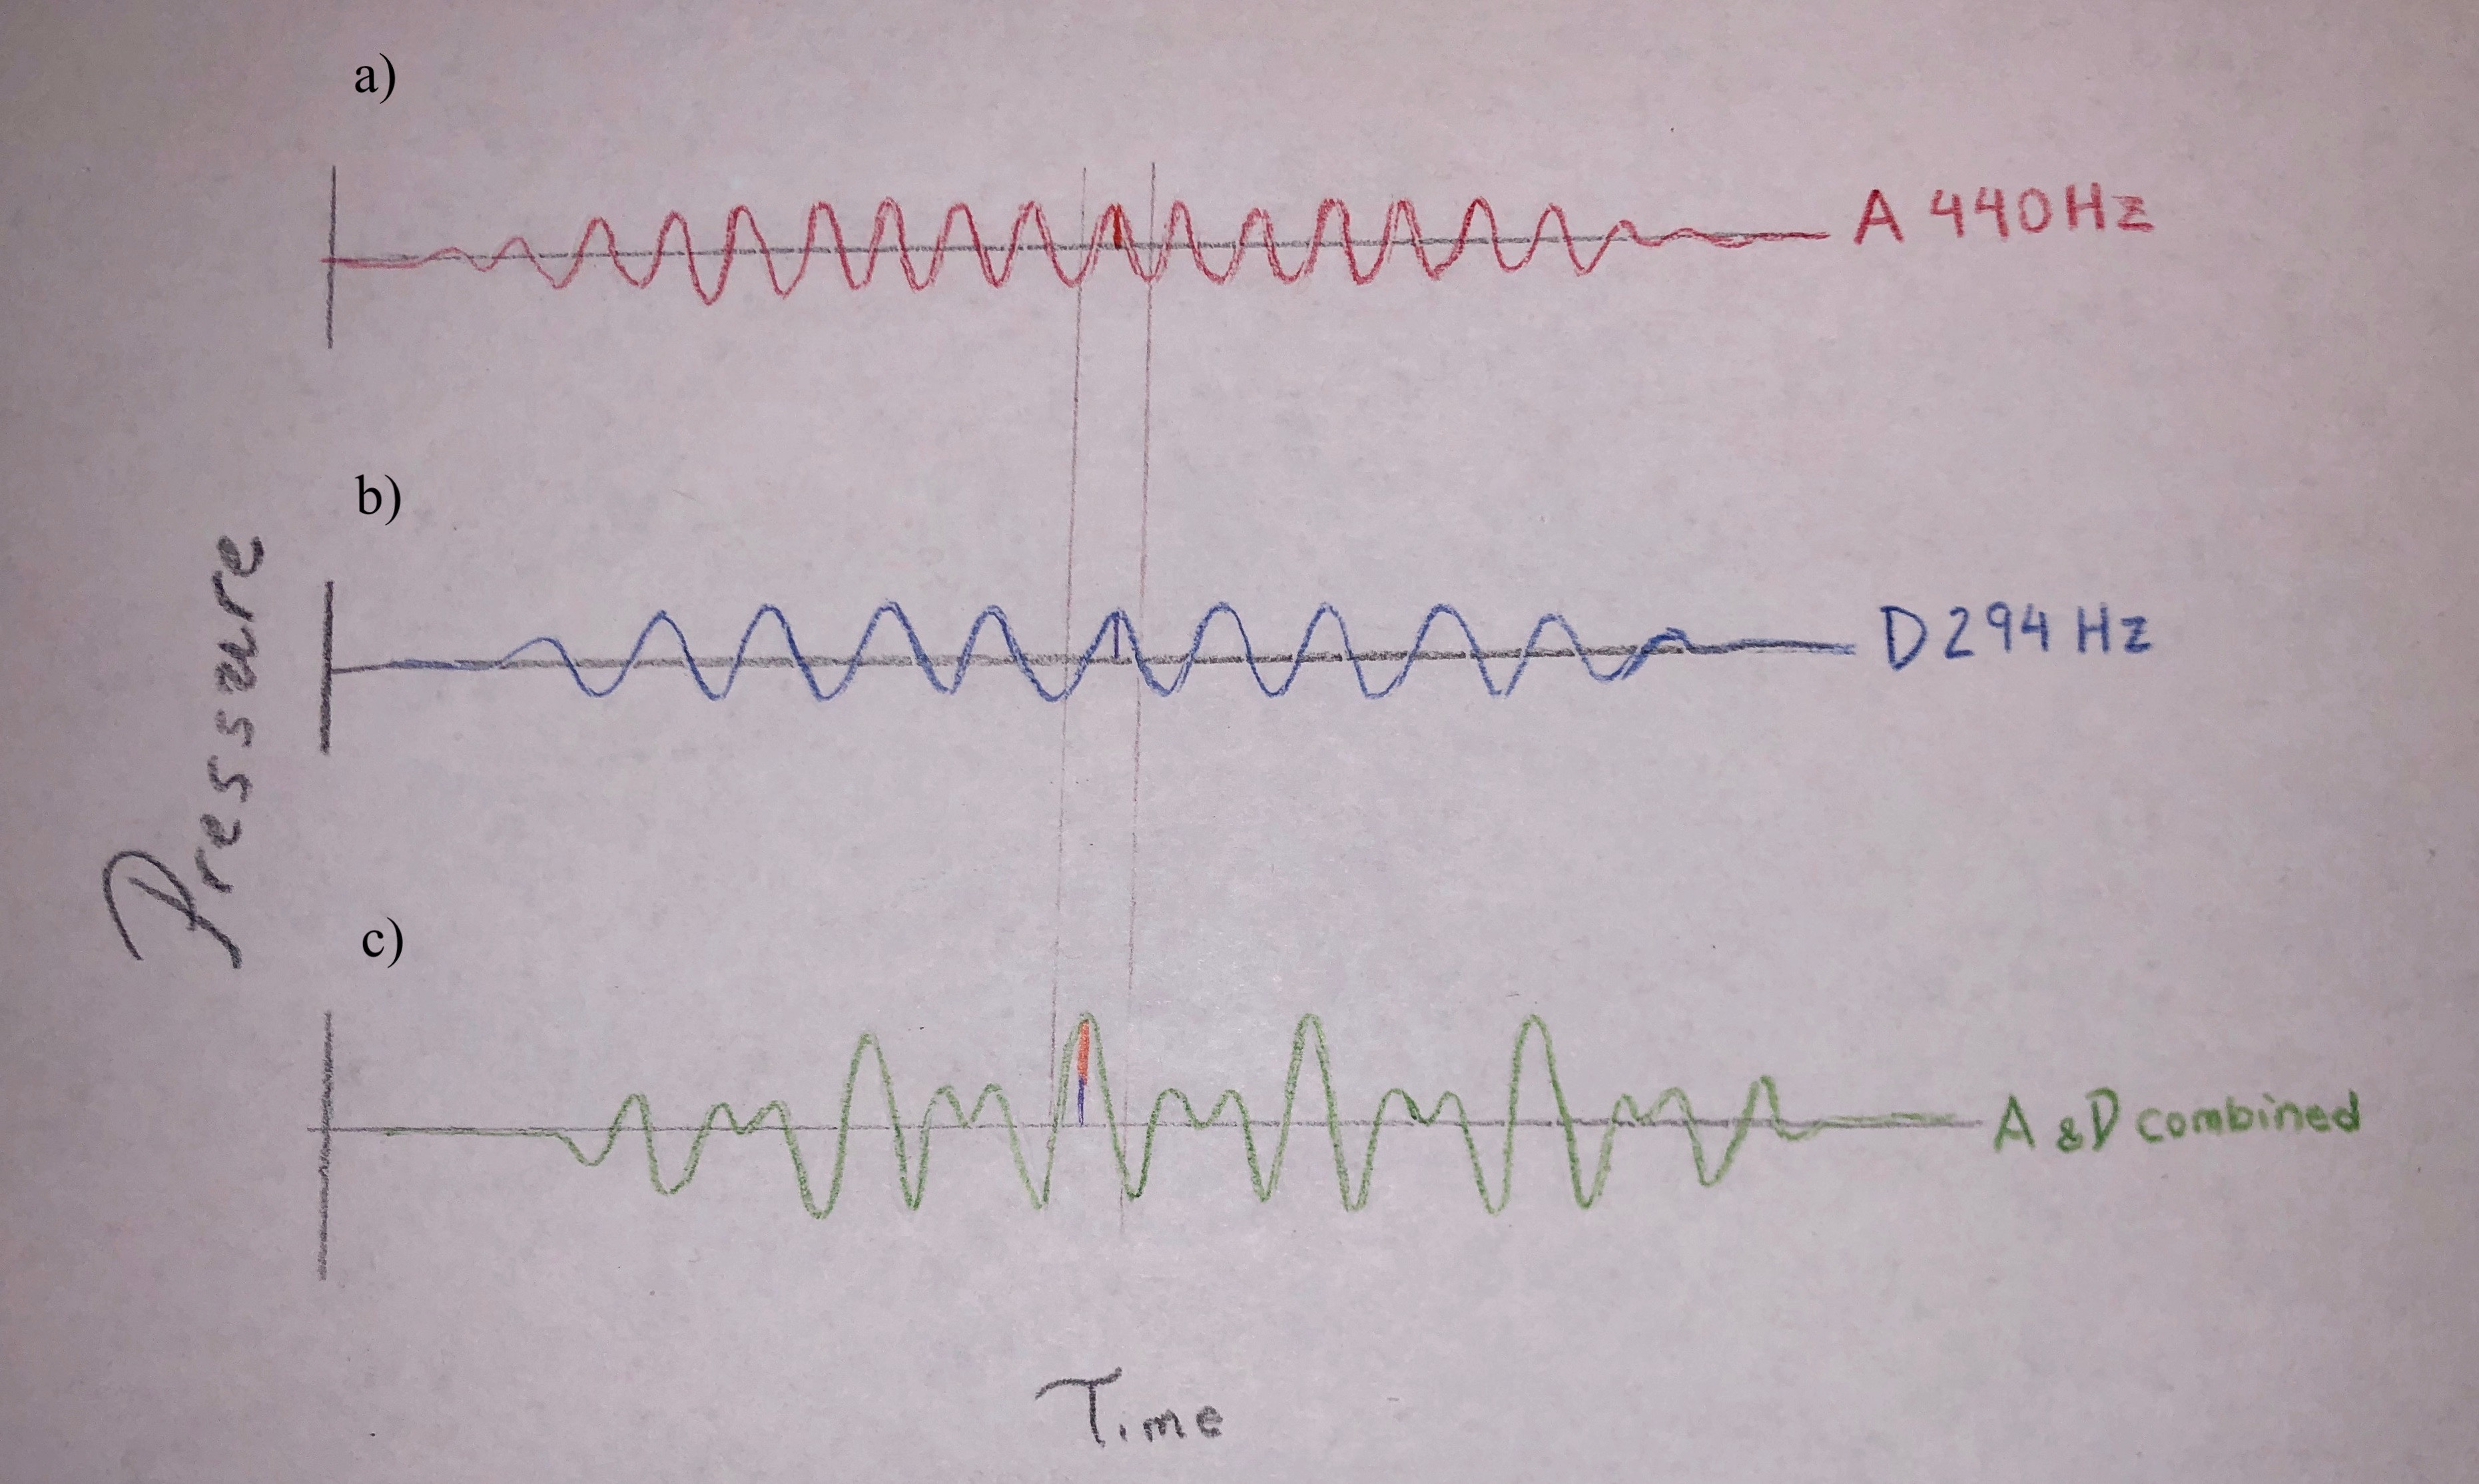
\includegraphics[scale=0.1]{frequencies.jpeg}
	\caption{A drawing of musical frequencies}
	\subcaption{ A drawing of the high frequency, 440Hz musical note,"A" or "La" (red);\textbf{(b)} A drawing of the lower frequency, 294Hz musical note,"D" or "Re" (blue);\textbf{(c)} A drawing of the additive frequency of notes "A" and "D" to produce an amplitude that is equal the additive amplitudes of "A" and "D" when constructive; Adapted from freely available lessons by 3Blue1Brown.}
\label{fig:frequencies of music} 
\end{figure}

A language exists, which is not subject to misinterpretation of translation, and that is the language of mathematics. From the first known records of mathematics which date back to approximately 3000 B.C.E. until now, what has been common between four sheep and four goats has always been their \textit{value}, equaling to 4. With common units of length, time, volume and the like, we can describe in exponential terms the quantitative scale of a value. Using mathematics, humans can describe the phenomena that we observe--from the attractive forces that govern the behavior of the smallest atom, to the revolution of planets in galaxies that are not our own. What is more, mathematics allows us to tease out simple formulas that \textit{predict} the future state of a system. 

To understand the power of mathematics, we must lend some consideration to the ability to \textit{visualize} mathematical concepts; an example best demonstrated by examining one of the most amazing phenomenon known to mankind: the musical genius of Beethoven, \textbf{a deaf man}. How could it be possible for a man who could not \textit{\textit{hear sound}} to produce such melodic masterpieces? The answer is purely, the visualization of mathematics. Ludwig van Beethoven once said, 

\begin{center}
    "I always have a \textit{picture in my mind} when composing, and follow its lines."
\end{center}

Ludwig van Beethoven was able to see and feel the mathematical relationship of musical notes relative to one another.  In his quote, he proved to be true the reality that so many non-traditional artists and scientists live: a deepened understanding of something is somehow tied to ones ability to visualize it in their mind's eye. As the famous mathematician, James Joseph Sylvester once said, 

\begin{center}
    "The musician feels mathematics, the mathematician thinks music: \\ music the dream, mathematics the working life."
\end{center}

Many of us do not know what it means to "visualize" music or mathematics. But, if you have the privilege of hearing, you may recognize the note commonly known as "A" or "La." If you used a pressure reader near the source of the sound of the note, the pressure recorder would record 440 beats per second, or 440 Hz. A visual form of this is the drawing shown in Figure 0.1. 


\section{Scaling up through the sciences}
Our knowledge about the world around us has its roots in mathematics. The application of mathematics to the laws that govern the physical world is termed, \textit{physics}. The laws and theories of physics applied to the study of matter are collectively, \textit{chemistry}. The use of chemical principles used to describe living systems is \textit{biochemistry}. All of these disciplines are common in their use of mathematics to prove the principles that are upheld by what we are able to observe. 

Oftentimes, biochemical systems become so complex that mathematical formulas become difficult to compute. For this, scientists use computational algorithms that describe and predict behaviors. But the more explicit we become in describing a system, come limits in computational power. In 1965, Gordon Moore published a paper entitled, "Cramming more components onto integrated circuits," \cite{Moore1965} where he first theorized about the relationship between the passage of time and the growth of computational power, known today as Moore's law. Over half a century later, our technological power has grown to a point where almost every person carries a small, powerful computer in their pocket, yielding access to volumes of up-to-date information at the mere decision of the user. Even still, biological systems are so complex and operate at such small time scales, that computational power is often the limiting factor in obtaining an answer to our questions. 

Nevertheless, using the computational power we can presently harness combined with sophisticated mathematical algorithms, we computational biophysicists have created a powerful tool, \textit{the computational microscope}. 

Like a true microscope, we can choose a "magnification" or scale to visualize that which our mind seeks to see. The invisible suddenly becomes visible. And most importantly, we can see the biophysical ramifications of small changes scale upwards through time. 

With humility, I ask the reader: Join me in this journey across scales of microscopic biophysical space-time to see the unseen, through the lens of the computational microscope. 

\section{The multiscale nature of biochemistry}
\setcounter{figure}{1}
\begin{wrapfigure}{r}{.37\textwidth}
    \begin{minipage}{\linewidth}
    \centering
    \captionsetup[subfigure]{justification=centering}
    \captionsetup[caption]{justification=centering}
    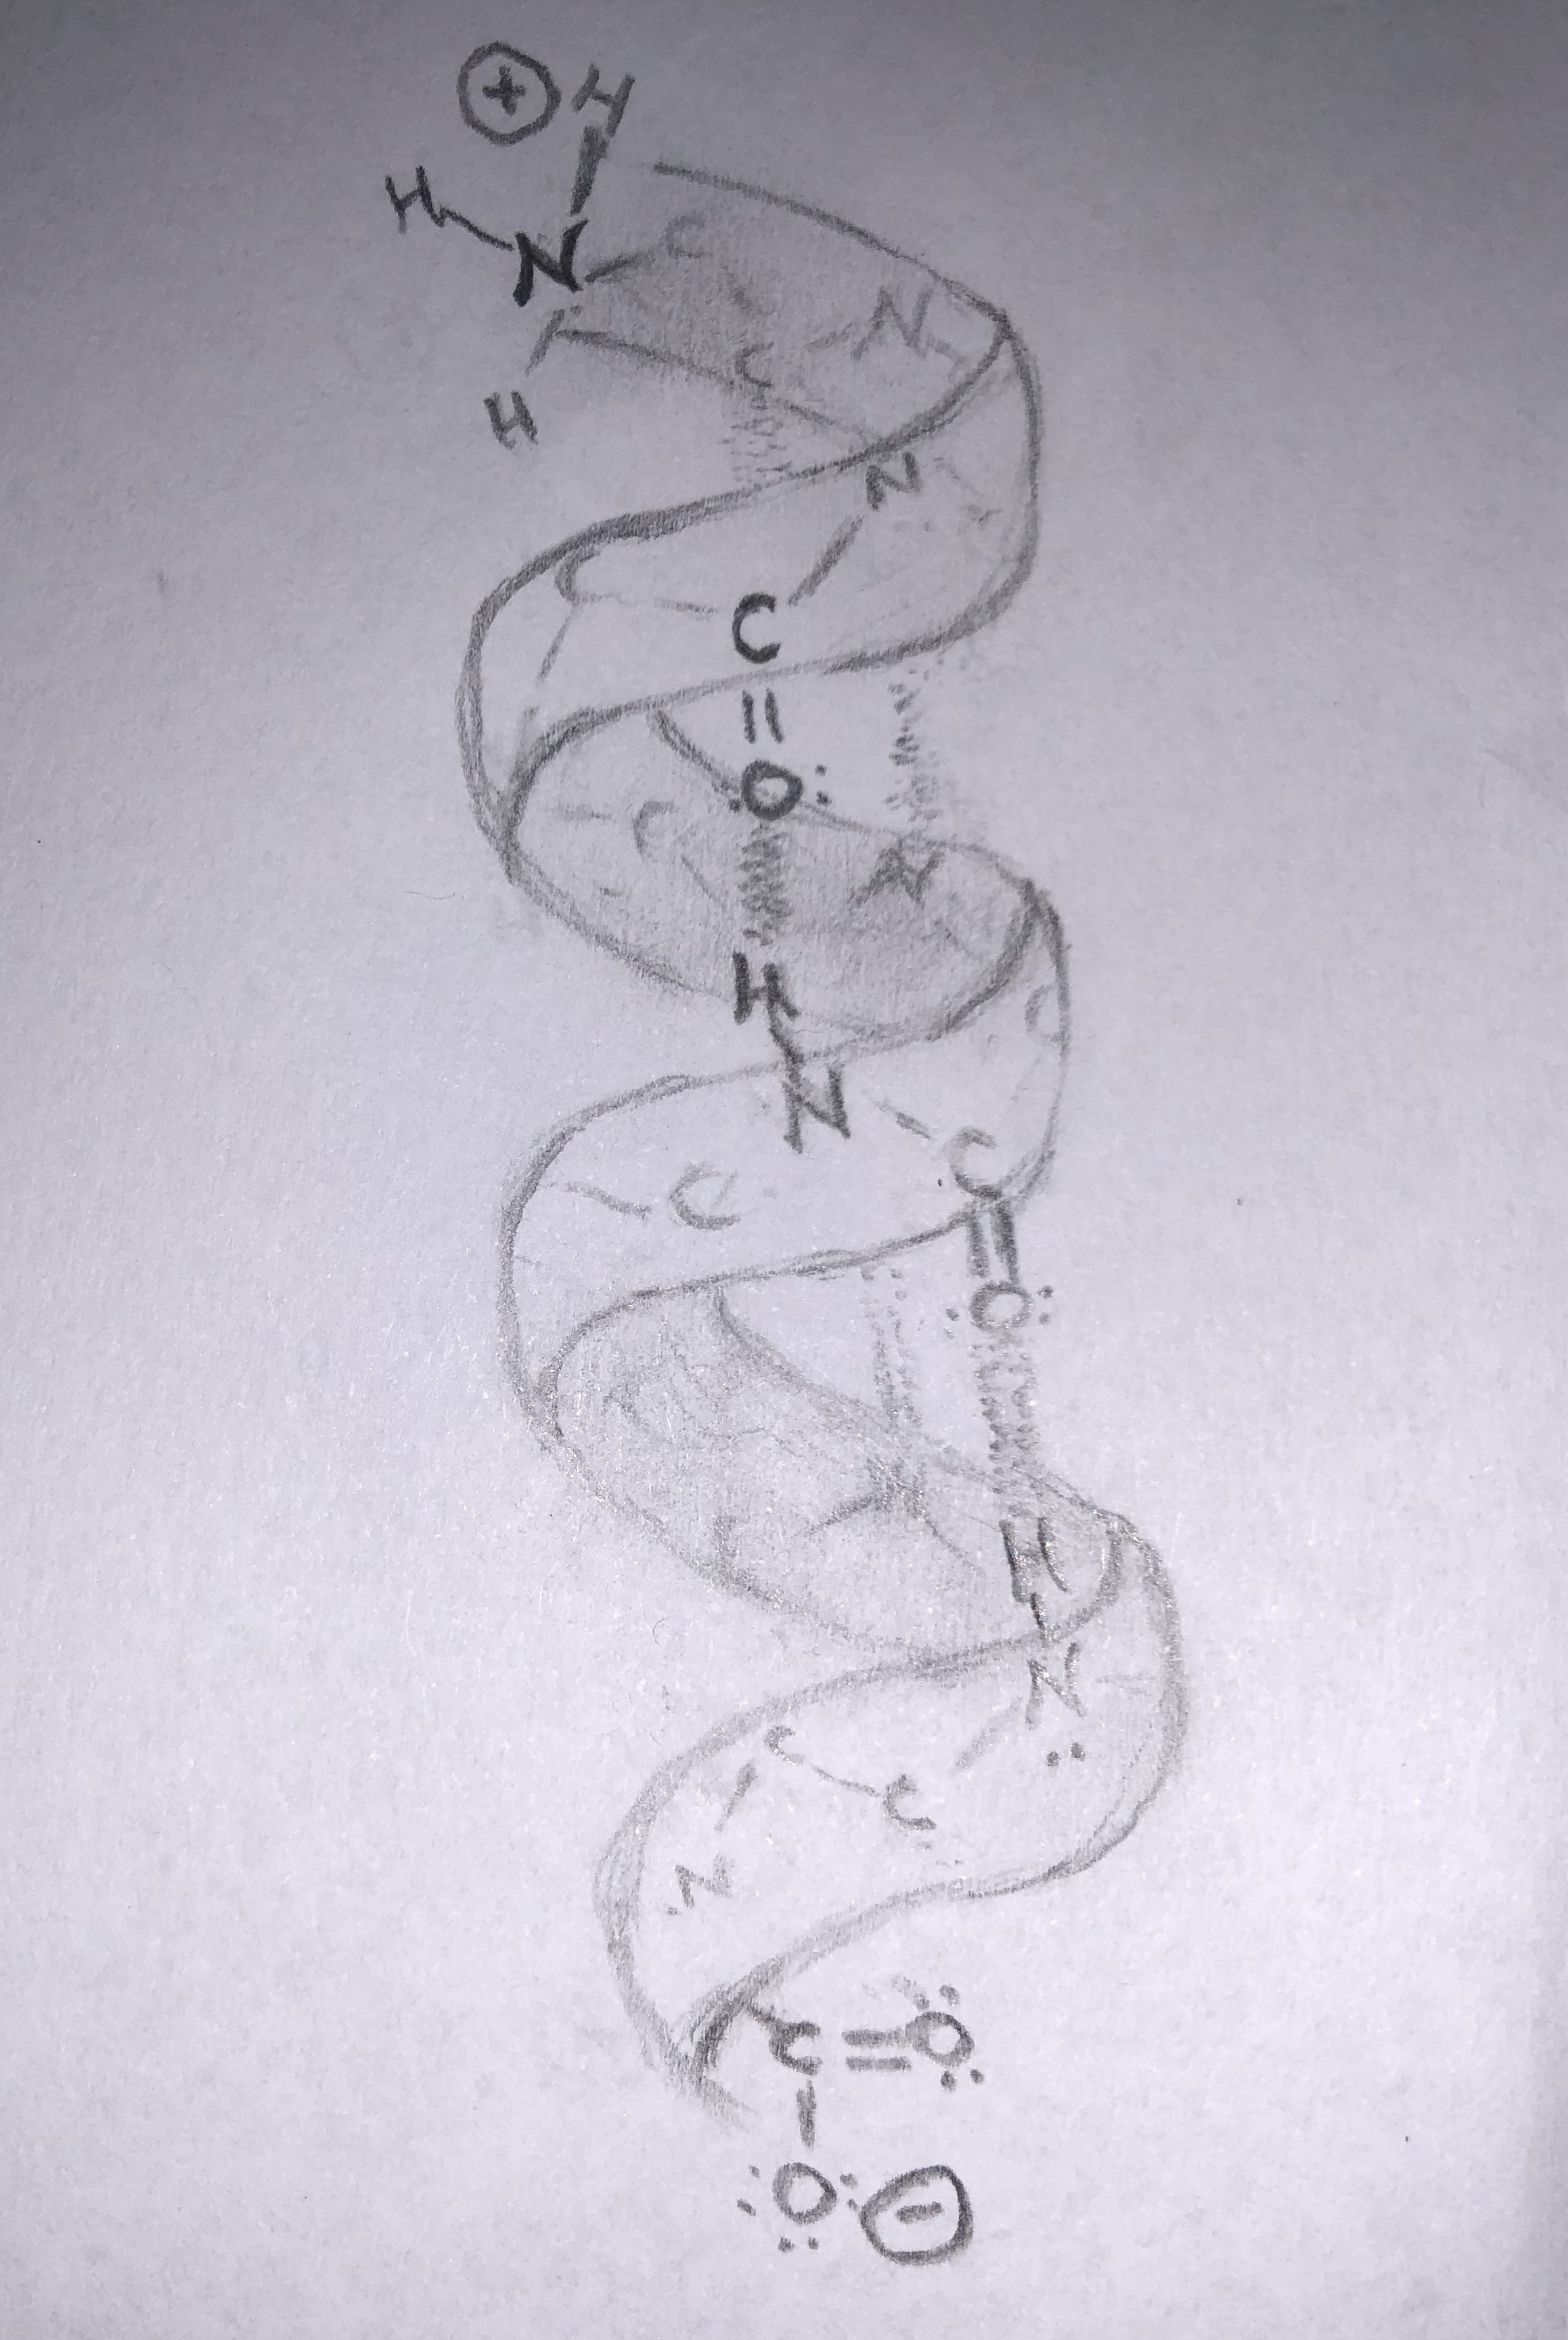
\includegraphics[width=0.55\linewidth]{helix0.jpg}
    \subcaption{$\alpha$-helix structure}
    \label{fig:0a}\par\vfill
    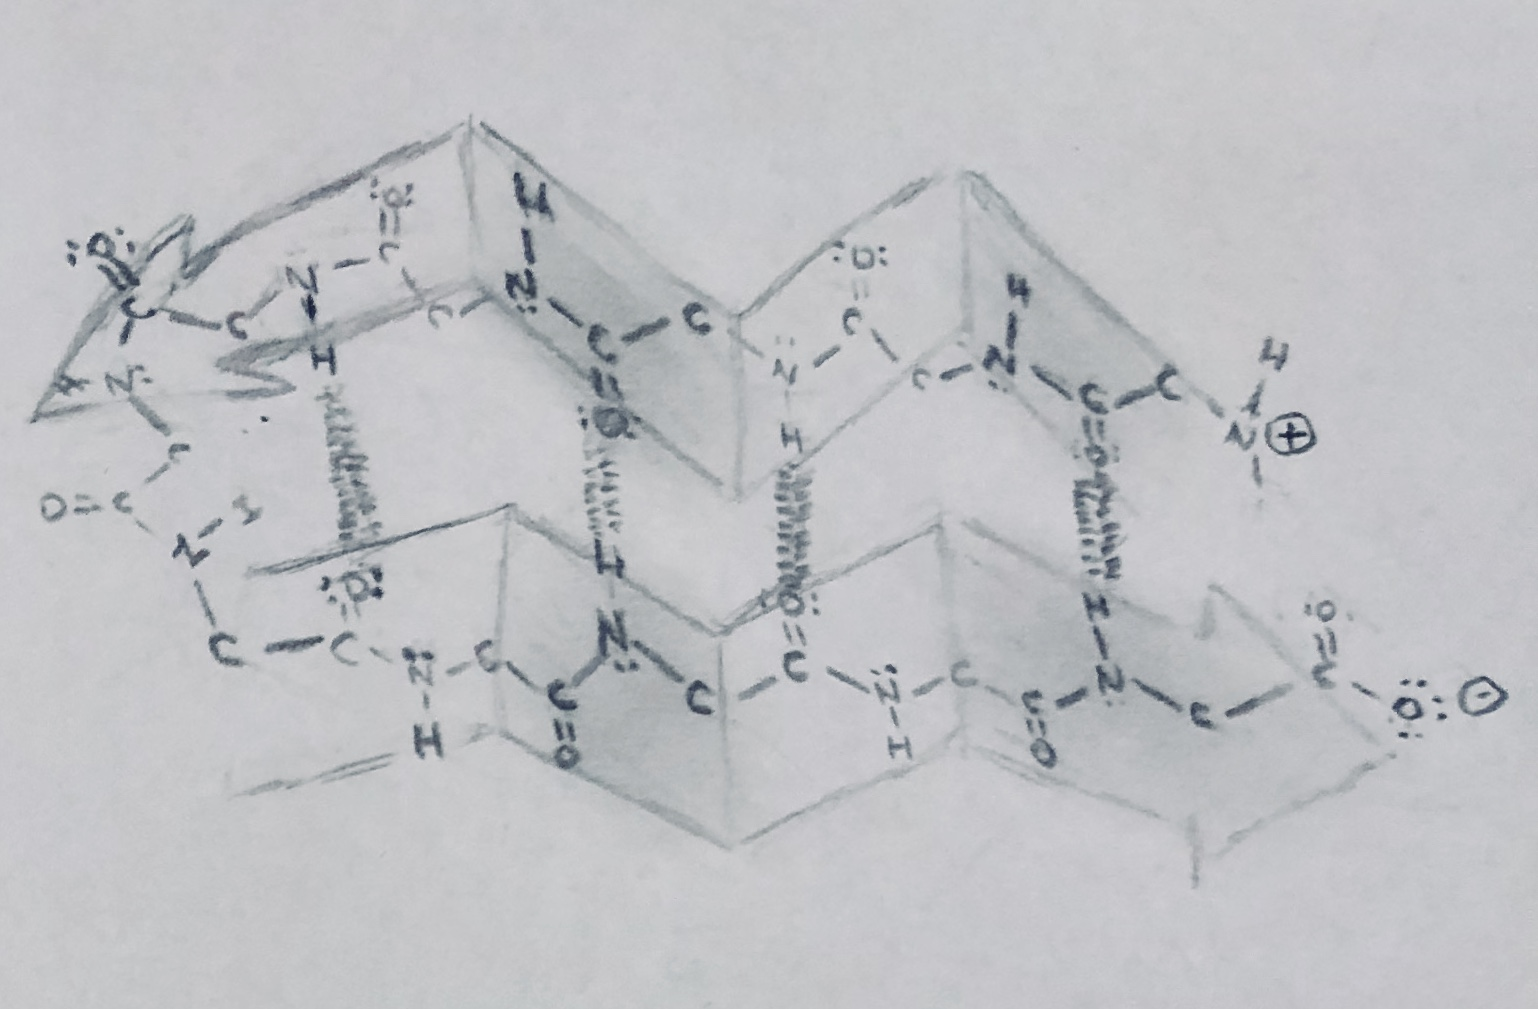
\includegraphics[width=0.8\linewidth]{sheet0.jpg}
    \subcaption{Parallel $\beta$-sheet structure}
    \label{fig:0b}
    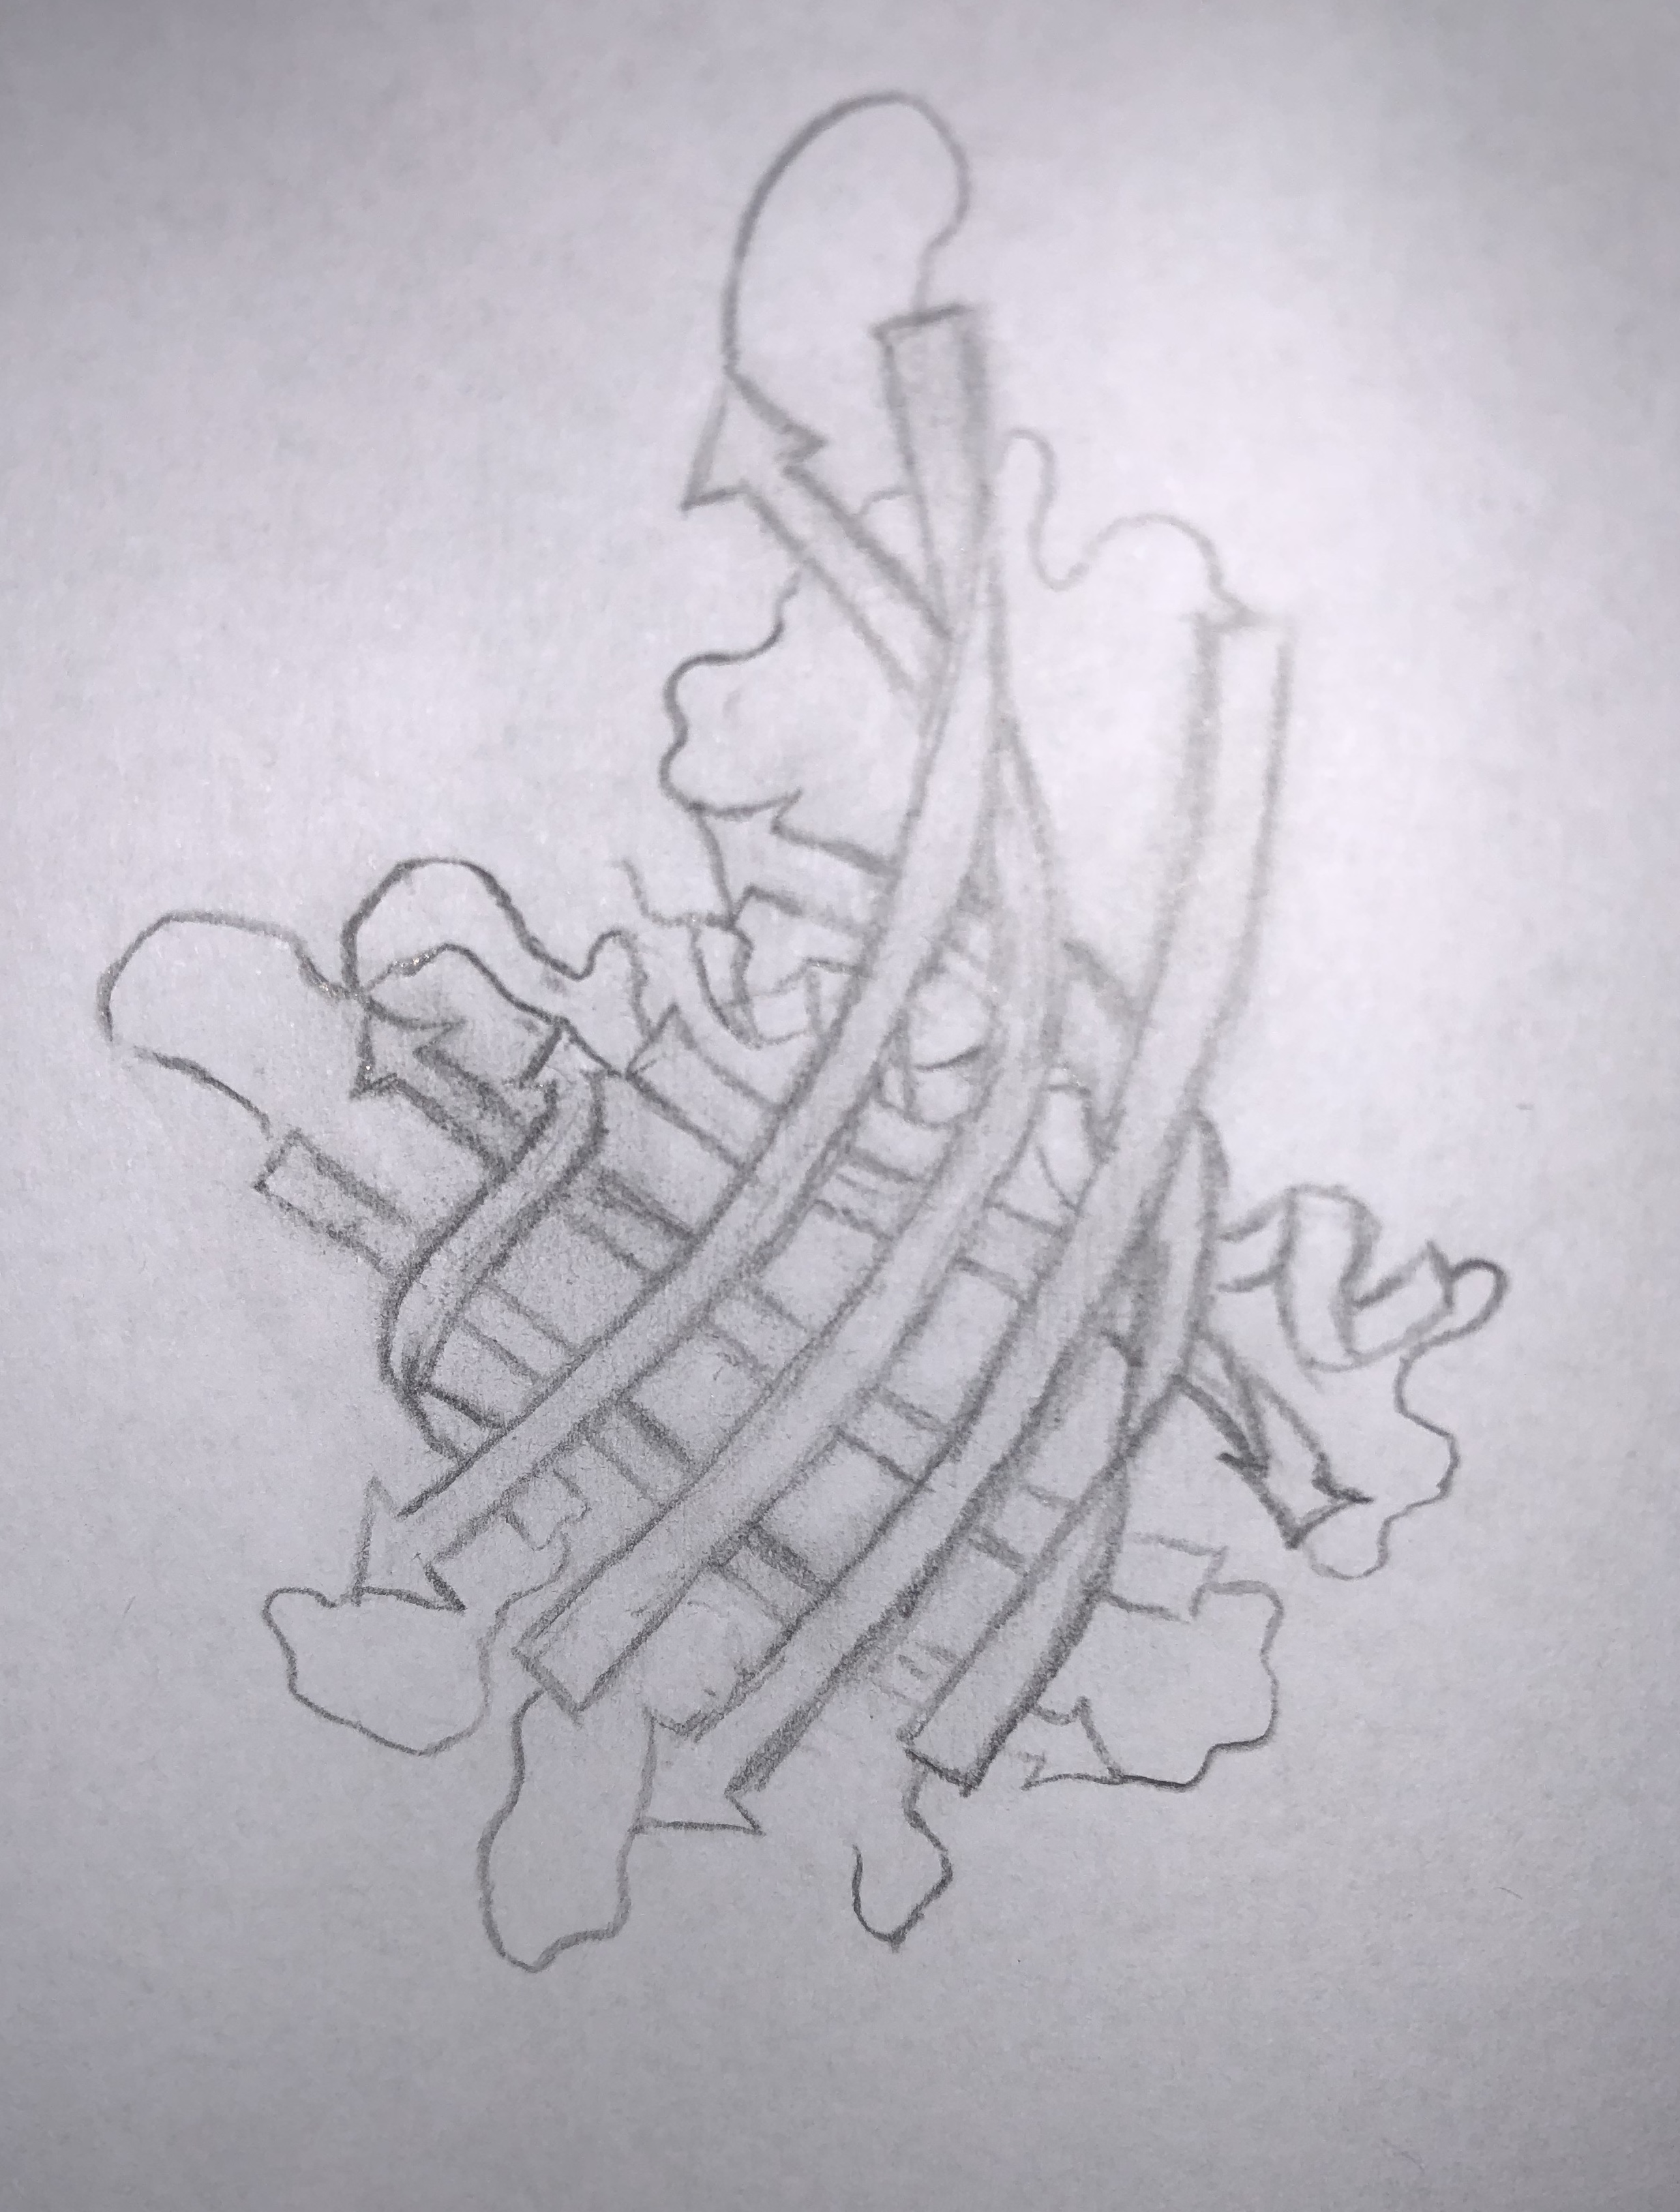
\includegraphics[width=0.65\linewidth]{tertiary0.jpg}
    \subcaption{Tertiary structure of a protein comprised of $\beta$-barrels and an $\alpha$-helix}
    \label{fig:0c}
\end{minipage}
\caption{Levels of protein structure}\label{fig:0}
\end{wrapfigure}

The complexity of biological systems stems from the various scales of space and time within which they operate. In terms of the field of biochemistry, there are many levels that operate in unison to produce an observable phenomenon. This section will describe the various mechanisms that underlie structure in biochemical systems.

Firstly, \textit{atoms}, joined by attractive forces called bonds, link together to produce \textit{molecules} called \textit{amino acids} (also known as \textit{residues}). Atoms come in different sizes and shapes but are generally on the order of 1x$10^{-10}$m (1\si{\angstrom}). There are twenty different amino acids, all differing in their side-chain structure and therefore, their physical properties. Each amino acid molecule has a common backbone which begins with a reduced nitrogen atom (amino) and ends with an oxidized carbon atom (acid) with a width of about 4\si{\angstrom}. Some amino acids are polar and charged, interacting with other charged species and water. Others are hydrophobic and "hide from water," through water-exclusion forces. These acid interactions dictate the structure or the "fold" of the protein. Figure 0.2 demonstrates the levels of protein structure: from hydrogen bonding in alpha helices (a) and beta sheets (b), to folds that result in tertiary structure (c).

The structure and dynamics of a protein are determined by its sequence. The amino acid sequence is specified by the genetic code of the organism, known as deoxyribose nucleic acid (DNA). Our DNA is \textit{translated} to messenger ribonucleic acid (mRNA) and \textit{transcribed} to the protein sequence. The linkage of amino acids in a linear "code" is known as the \textit{primary structure} of a protein. When the protein chain lengthens, the protein backbone folds onto itself using non-bonding interactions between the backbone hydrogen and oxygen atoms called hydrogen bonds. This causes \textit{secondary structure} like $\alpha$-helices and $\beta$-sheets to form (see Figure 1a,b). Collections of secondary structural moieties lead to the formation of \textit{tertiary structure} (see Figure 1c). A collection of proteins within the same system is called a complex with the individual proteins known as subunits. For example, a protein complex of two regulatory (R) and two catalytic (C) subunits can be written as R$_{2}$C$_{2}$. Two or more subunits within a complex is termed the \textit{quaternary structure} of the protein. Different quantities and arrangements of the same subunits can have different structures and functions. Thus, quaternary structure yields multiplicity in the number of structures a single protein complex can have. 

A slight change in amino acid sequence can alter the \textit{structure} of a protein drastically, and oftentimes, affect the \textit{function}. For example, residues like Glycine (G) confer lots of flexibility in helices, often causing helices to break reversibly. A simple mutation to a more-rigid residue like Proline (P) are leads to a turn in the sequence and this, can break a helix without allowing for flexible return to helical moieties. Mutations thus oftentimes affect the way the protein moves and interacts with other molecules, leading to large-scale changes signaling cascades on the cellular level. Such is true with changes in expression levels of DNA, RNA, proteins, In this way, atomic-level alterations can have a \textit{butterfly effect}, leading to the presentation of disease phenotypes in the organism that harbors the mutation. 

Protein Kinase A (PKA), one of the systems examined by this thesis, is a prime example of a case in which a single-point mutation can alter structure and is discussed in more detail below.

\section{How mutations affect protein structure: a multiscale biologist's perspective}

Protein Kinase A is found in every multicellular organism. It is responsible for responding to extracellular signals and eliciting an intracellular response; a signal translator and amplifier of sorts. PKA binds a molecule named cyclic adenosine monophosphate (cAMP) in the cyclic-nucleotide binding domain (CBD) regulatory subunit. Once enough cAMP is bound to PKA, the regulatory subunit relieves its inhibition on the catalytic subunit, which is responsible for phosphorylating protein targets, effectively deactivating or activating them in response to an extracellular signal. This tightly controlled mechanism is vital to the function of the cell. Any dysregulation in the response of PKA has major detrimental effects that are common in cancer \cite{Caretta2011}, XX

A positively charged reside in PKA, Arginine (R) in position 333 of the regulatory subunit interacts directly with the first molecule of cAMP sensed by PKA. Because of its flexibility, the tetrameric for PKA RI$\alpha$ structure has proven difficult to elucidate [cite], but scientists figured out that with a mutation of R333, the dynamics of PKA are stabilized enough for structural biochemists to be able to visualize it.

\begin{figure}
\centering
	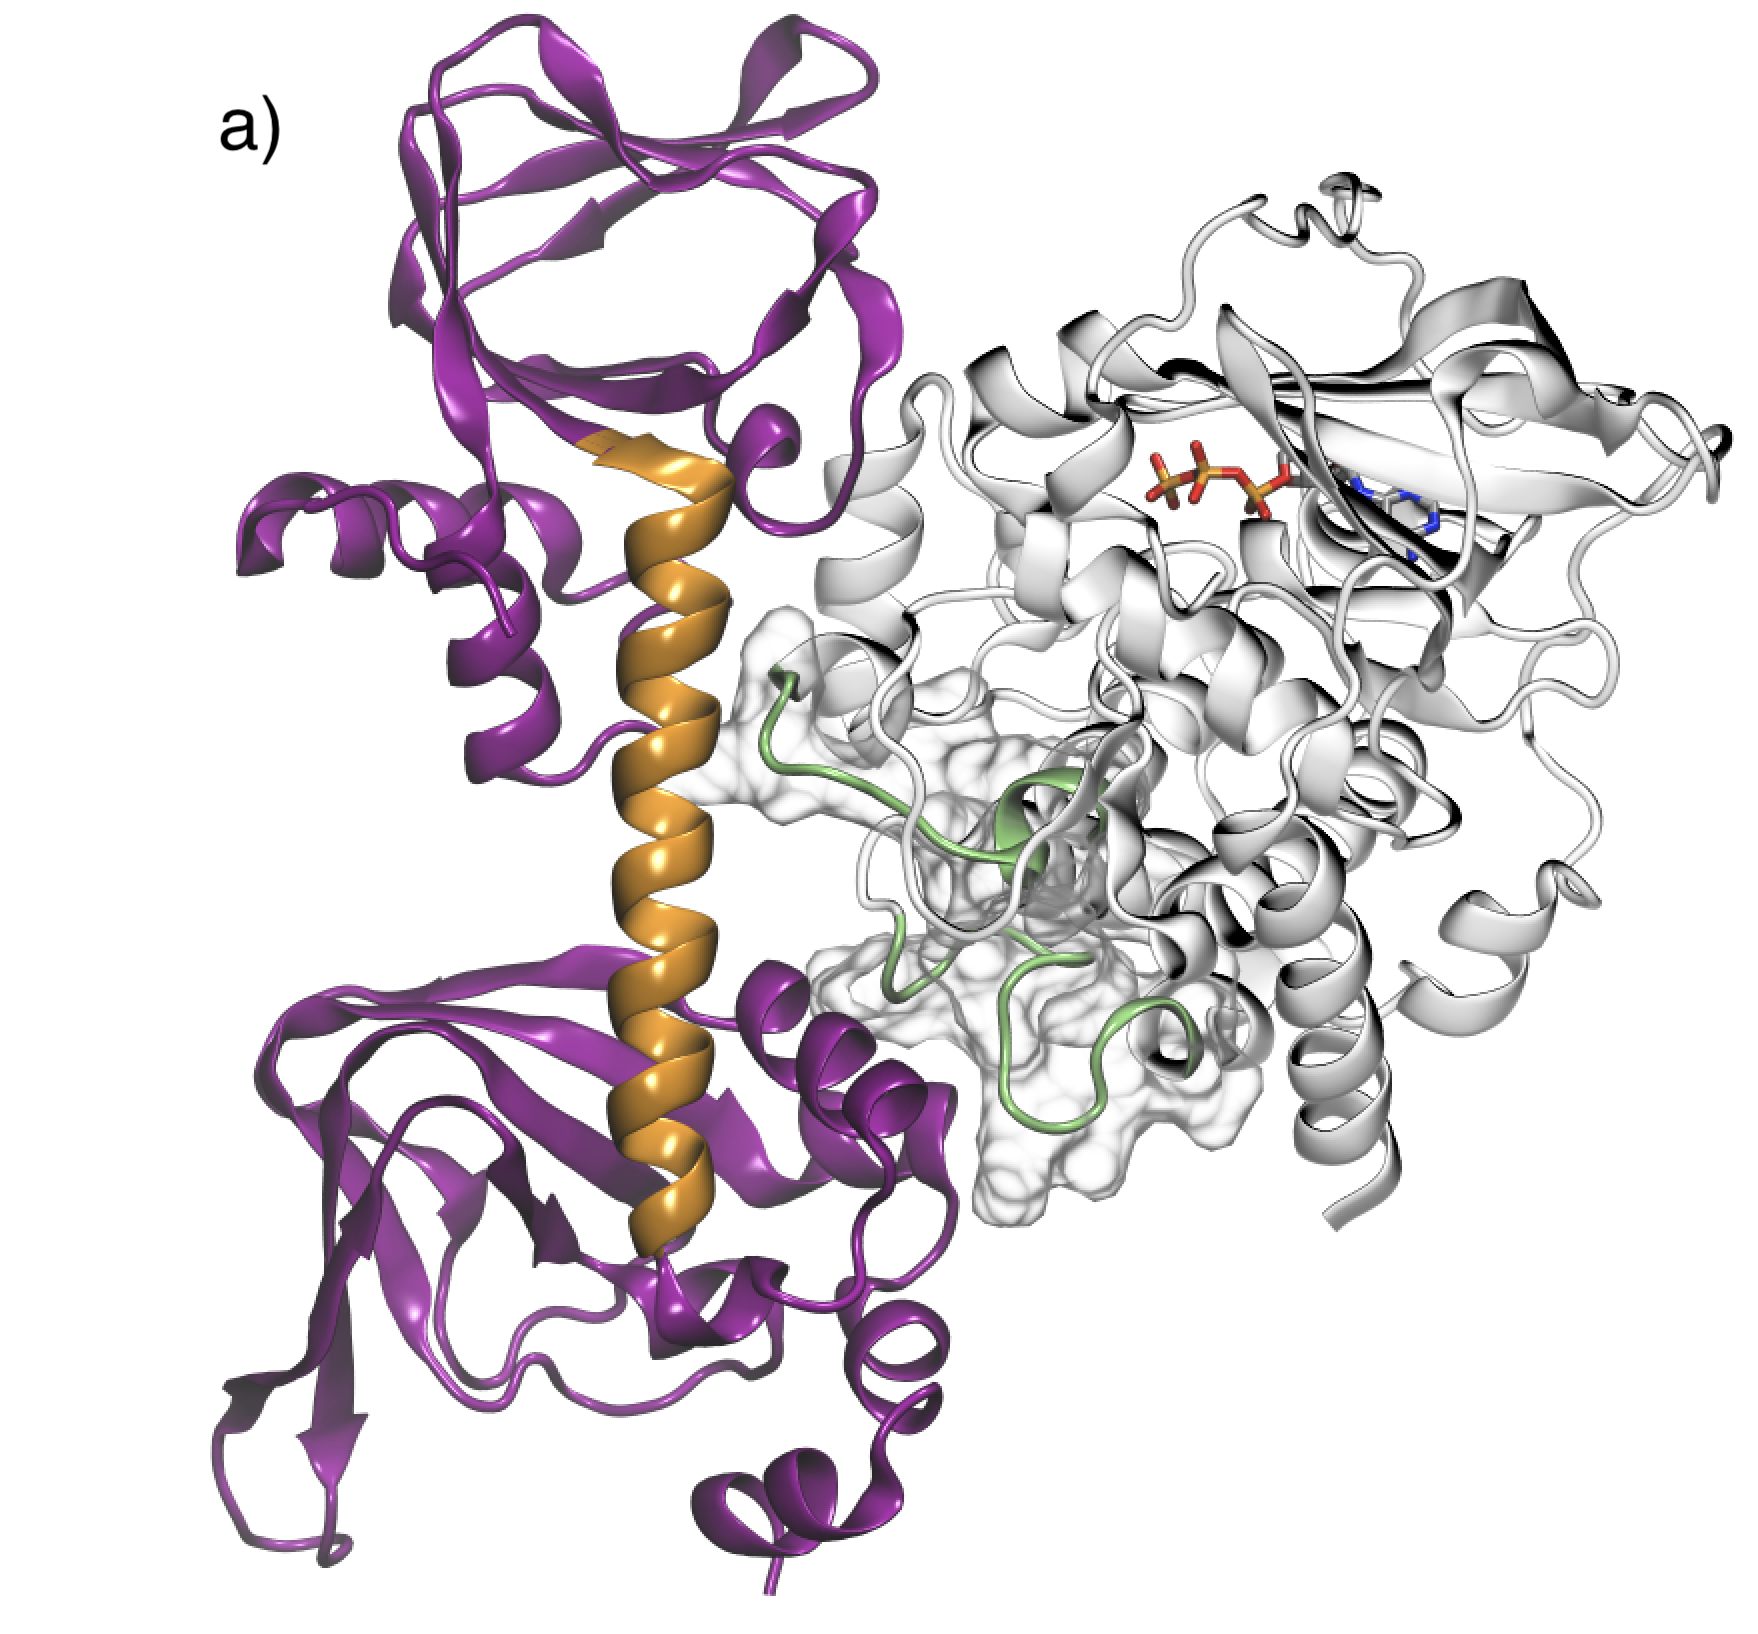
\includegraphics[scale=0.22]{RC_PKA_holo.png}
	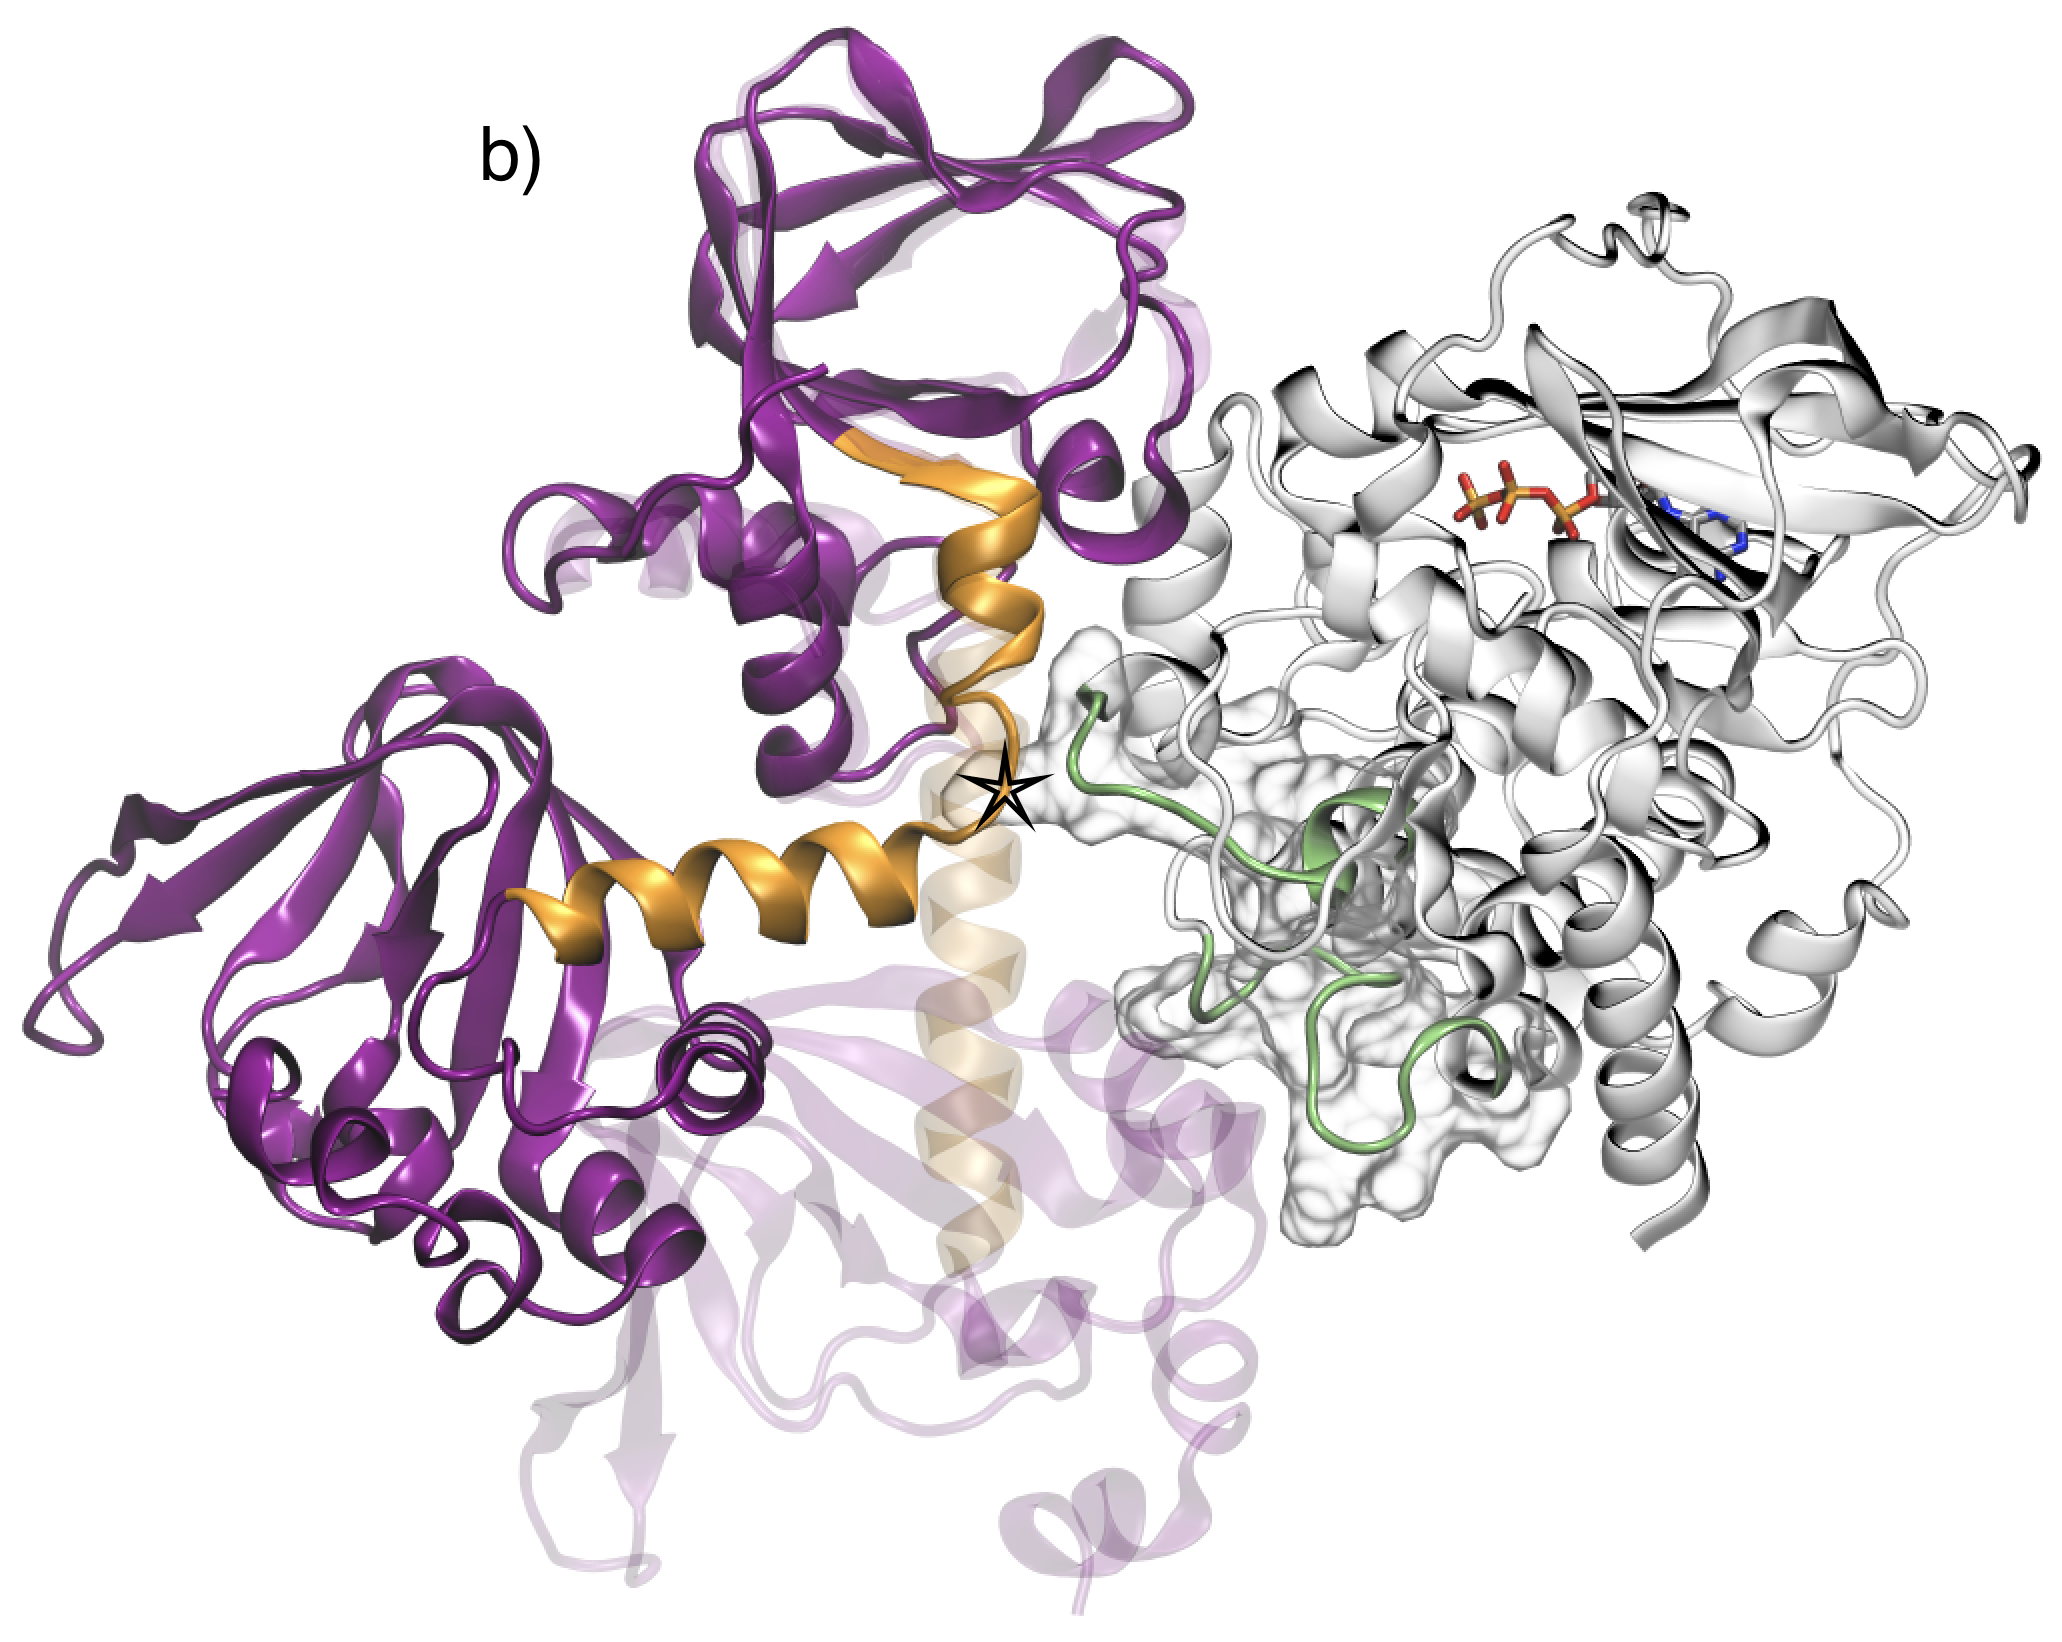
\includegraphics[scale=0.22]{RC_PKA.png}
	\caption{The interface of the Regulatory and Catalytic subunit of Protein Kinase A (PKA), comparing the mutant to the wild-type}
	\subcaption{The mutant Regulatory subunit (R) R333K (purple)  in complex with the Catalytic subunit (C). The B/C helix (gold) connecting the two cyclic nucleotide binding domains (CBDs) is extended in the heterodimeric crystal structure; \textbf{(b)} The wild-type R subunit adopts a stable conformation with a break in the B/C helix at Glycine 235 (black star). The structure is juxtaposed with the R333K mutant (transparent purple) to show the consistency of the WT conformation with the solvent-exposed regions in the C subunit (green) determined by solution experiments}
\label{fig:RC} 
\end{figure}



 When R333  is mutated to a Lysine (K), which is \textit{also} positively charged, the shape of the PKA molecule changes not slightly, but drastically (see Figure 0.3). This mutation also affects PKA function, altering the way the protein responds to the cAMP signal. In the wild-type (WT) R333 case, the protein is dynamic, with a swinging protein domain that creates a butterfly motion in the protein. It responds to cAMP by dissociating the regulatory subunit from the catalytic subunit, relieving inhibition and activating PKA. In contrast, the K333 mutation makes the protein more globular, neutralizing the motion of swinging domain\cite{Cheng2009} and changes the interaction between cAMP and the regulatory subunit, completely altering the way that PKA is activated. This and other mutations are known to be the root cause of diseases like Carney complex\cite{Kirschner2000} and Adrenocortical Cushing’s adenoma\cite{Calebiro2014}. In this way, a single residue mutation effects the dynamics of a protein, and the way that the protein interacts with its environment. 


\section{Structural Methodologies}

As the specialization of this degree is centered on Multiscale Biology, the following chapters will discuss experiments that utilize information gathered from different structure elucidation methods with range in spatial scales from small molecule (\si{\angstrom}), to proteins (nm), to membranous structures on the sub-cellular level ($\mu$m). The following section is review these methodologies for biological structure determination and alludes to the ways these methods facilitated scientific investigations in the coming chapters. 

\subsection{X-ray Crystallography}
Crystal x-ray diffraction or Crystallography is popular and widely used method for determining atomic-level positions of small molecules and proteins. First developed in 1912 by Max von Laue and later further developed by William Henry Bragg and Sir William Lawrence Bragg \cite{Bragg2014}, crystallography is based on the principal of X-ray diffraction by the atoms in an ordered crystalline substance. 

As the name indicates, the subject of interest is suspended in a crystallographic form and a beam of X-rays is shot at the sample. Using the angular positions of the diffracted X-ray beams and a mathematical equation known as the Bragg equation:

\begin{equation}
n\lambda=2d\sin\theta
\end{equation}
Where n is an integer multiple of the wavelength, $\lambda$ of the X-ray beam, while d is the distance between the planes of the crystals, and $\theta$ is the scattering angle. From the interference and diffraction pattern produced by the X-ray beam after hitting the crystal lattice structure, one can back-calculate atomic positions. 

X-ray crystal structures yield \si{\angstrom}-level resolution of structure; a real asset for computational chemists and biophysicists who use the atomic positions as inputs for their models. Section 0.4 of the introduction will elaborate more on how atomistic positions are used to understand dynamics and functions of small molecules and proteins. 

It is important to note that an X-ray structure is but a snapshot of a molecule in a single state of its ensemble of conformational states. Although crystal structures are unparalleled in their accuracy of single structure, by nature, they do not give information about molecular flexibility.  Furthermore, the resolution of atomic positions falls off as molecules increase in size. Therefore, crystallography is limited in the size of the molecules that can be investigated with sufficient accuracy. For this, X-ray structures can be complimented with other structural determination and computational methodologies, further discussed in the coming sections. 

Chapter 2 combines X-crystallography with molecular dynamics in an investigative study of common structural motifs used by an infectious organism. In Chapter 3, we will explore the caveats of crystallography and show how molecular dynamics can expand on structural information not offered by these snapshots of proteins. 

\subsection{Hydrogen/Deuterium Exchange Mass Spectrometry}
A remedy for the limited structural ensembles that can be understood with X-ray crystallography is Hydrogen/Deuterium Exchange Mass Spectrometry(H/DxMS).  Since the discovery of the "heavy" hydrogen isotope, deuterium in 1932 by Harold Urey et al. \cite{Urey1932}, Deuterium has been used in a myriad of experimental techniques. Early in the 21st century, the application of the Deuterium to the study of proteins appeared \cite{Engen2001}. 

As indicated by the name, in H/DxMS, Hydrogen and Deuterium exchange (H/Dx) for one another. This happens specifically with labile Hydrogen atoms on the backbone nitrogen, which exchange nearly instantaneously.  In a solution of D$_{2}$O (the Deuterium version of H$_{2}$O), exchange is rapid if backbone Nitrogen are surface-exposed or located in an unstructured region of the protein, and slower if the nitrogen is buried in the core of a dynamic protein. Exchange can happen at a rate on the order of milliseconds to seconds if amide nitrogen are not hydrogen bonded, but can take minutes to days if hydrogen bonds are stable. Timescales of exchange are translated to the  "degree of protection" of the amide and indicate the degree of dynamics and structure of the protein itself.The exchange reaction of hydrogen for deuterium is then quenched by acidification of the protein (pH ~ 2.5), which serves to "freeze" the deuteration of the protein.  Proteolysis then follows-- a method that degrades the protein into smaller fragments to be analyzed by Mass Spectrometry (MS). Mass Spectrometry determines the atomic weight of the fragments, yielding the information of which nitrogen have exchanged their hydrogen for deuterium \cite{Konermann2011}. 

This technique is used to understand the comparative changes in dynamics induced by protein-protein interactions, ligand binding, as well as signaling modes of a protein\cite{Harrison2016}. H/DxMS yields a \textit{dynamic} picture of the protein, allowing biophysicists to understand the flexibility of a protein. Moreover, the technique is less limited in the size of molecules that can be investigated. 

This method compliments computational methods like Molecular Dynamics which explore conformational ensembles of proteins. Chapter 3  details how H/DxMS in combination with Molecular Dynamics have brought us closer to a more holistic understanding of the structure of a protein complex, as was briefly discussed earlier. 

While X-ray crystallography and H/DxMS give information about local protein structure, the following methods give insights about global structural features of proteins. 

\subsection{Small-Angle X-ray Scattering}
As discussed earlier, X-ray crystallography utilizes the diffraction, or "bending", of X-rays to resolve the atomic positions comprising molecular structure. But X-rays can also interact with a sample, altering the momentum of the beam in a phenomenon known as \textit{scattering}. In the phenomenon of scattering, the photons in an X-ray beam interact with electrons in a biological structure. The scattering pattern indicates the fluctuation of the electron density of the matter being investigated. Put more simply, the scattering profile gives information about the overall shape of a molecule. This is accomplished by measuring the scattering profile in the following way: a photon of wavelength $\lambda$ scatters off the molecular sample at an angle, 2$\theta$ is related to the scattering vector, q through equation 2. The intensity of the scattering vector, I(q) is a function of a multitude of factors, including molecular volume, size, electron density. 

\begin{equation}
    q = \frac { 4 \pi \sin ( \theta ) } { \lambda }
\end{equation}

The elegant mathematical theories used to obtain information SAXS experiments are summarized by experts in the literature \cite{Boldon2015}, but to summarize: experimental scattering profile, information such as the molecular weight, molecular volume, and radius of gyration can be determined. What is important to note is that SAXS provides information about an ensemble of structural states, in stark contrast to X-ray Crystallography, which resolve explicit conformations of a molecule. This means that multiple structural states can be "lumped" together in the same SAXS profile if a molecule is flexible. 

 Molecular structure is, by nature, affected by its environment. SAXS has been used to understand molecular structure under particular conditions such as temperature, pH\cite{Carvalho2012}, and in complex with other molecules and proteins\cite{Cheng2009}. Thus, SAXS profile of a protein in its apo or "unbound" state will undoubtedly differ from its profile in a "bound" complex with a small molecule, another protein or even another copy of the same protein. 
 
 In the same way, mutations can affect molecular structure resulting in different SAXS profiles when compared to wild-type (WT). Such is the case of a system examined in chapter 3 of this thesis. Using SAXS as a guide, we contextualized the crystallographic structure of PKA combined with the H/DxMS in order to validate the existence of an unresolved conformation of the regulatory subunit, the Flipback conformation.
 
 As is the true with most technologies, crystallography and solution-structure methodologies like H/DxMS and SAXS crystallography have their limitations. That limitation being, molecular size. As the molecular size increases, so often does the difficulty in resolving fine details from the system. Nevertheless, as we move up through spatiotemporal scales, we can utilize new methods that take advantage of different technology to gain insight into larger systems. 
 
\subsection{Cryo-electron Microscopy}

Just two years ago, the 2017 Nobel Prize in chemistry was awarded to Jacques Dubochet, Joachim Frank and Richard Henderson for the development of Cryo-electron microscopy (Cryo-EM) in resolving structures of biomolecules in solution. Cryo-EM utilizes an electron beam as an illuminating source to visualize proteins and large molecular species that are flash-frozen in their native structural states. 

Cryo-EM remedies the "single crystalline conformation" limitations of X-ray crystallography and combines the strength of solution structural methods that describe ensembles of structural states, as discussed in the earlier introductory sections. The ingenious method behind Cryo-EM completely avoids crystallization of biomolecules by flash-freezing the subject of study in aqueous solutions. This method, also known as vitrification was developed by James Dubochet along with Jean Lepault nearly 40 years ago \cite{Dubochet1982,Lepault1983,Lepault1986}. The original spray-freezing method evolved further with the use of high-pressure which increases the depth of vitrification \cite{SARTORI1993}. 

Vitrification involves cooling the sample to very low (cryogenic) temperatures thus, embedding it a glass-like, irregularly frozen vitreous state upon treatment with liquid ethane. This is a significant advantage over X-ray crystallography, as many proteins will not crystallize easily due to the inherent dynamic nature of proteins in general. It is also especially advantageous for membrane proteins which are notoriously hard to crystallize.

\setcounter{figure}{3}
\begin{figure}
\centering
	\includegraphics[scale=0.23]{SERCA_RyR.png}
	\caption{Angstrom-level representations of biomolecules} The Sarco/Endoplasmic Reticulum Calcium-ATPase, SERCA2a, (PDBID:5MPM) crystallized at 3.3\si{Angstrom} resolution (green, left) and the Ryanodine Receptor, RyR2, (PDBID:5GOA) resolved at 4.2\si{Angstrom} with Cryo-EM. 
5MPM
\end{figure}

Cryo-EM is a popular method for understanding the structure large proteins which can be too "noisy" for solution experiments like H/DxMS and Nuclear Magnetic Resonance\cite{Ishima2000}. In fact, the larger the system, the more intriguing the results of Cryo-EM can be \cite{Frank1995,Lee2015,Sevvana2018}. Figure 0.4 compares the size of SERCA2a, a protein that was resolved using X-ray crystallography at 3.3\si{angstrom} and RyR2, a large (>2MDa) protein at 4.2\si{Angstrom} with Cryo-EM.

The larger the system, the more possible projections of the molecule that can exist. This is because molecules are not oriented when they are captured in vitreous water. Thus, part of the "magic" of Cryo-EM stems from its use in resolving information from randomly oriented molecules. 

Our ability to visualize dynamic, large, and complex structures is a direct result of Joachim Frank's work in analyzing and processing the images derived from Cryo-EM \cite{Frank1970}. The algorithm, known as "cross-correlation," averages ensembles of structural states to resolve what is known as a "single-particle reconstruction" of a biological specimen \cite{Saxton1976}. Using several thousand 2D images of the same molecule in random orientations, the algorithm generates 3D reconstructions from 2D projections\cite{Frank2009}. 

Cryo-EM gives molecular detail on the order of several \si{angstrom}. The size-limitation problem still stands however: the larger the protein, the lower the atomic resolution will be. But the popularity of this method has and will undoubtedly continue to drive the development of both Cryo-EM and the algorithms used to resolve molecular structures. One can only hope that the resolution will improve, yielding atomistic detail. In the context of this thesis, Cryo-EM structures gave us insights into the subcellular context of large structures like the Ryanodine Receptor. The likes of which will be discussed in Chapter 4. 

\subsection{Electron Tomography}
As we scale up from atoms to molecules in living systems, the next "step" is towards the realm within-which we can see the direct effect of proteins, also known as the "subcellular" scale. The name, "subcellular," alludes to the fact that this scale is only part of a cell. At this level, organelles-- boundaries that distinguish specialized regions of the cell--become the subject of focus. 

To see "within" the cell, 

\section{Biophysical Structural Modeling Methodologies}
Studying the dynamics of proteins is no simple feat. Proteins are incredibly small and their relevant motions are fast. The oftentimes too fast to study with available technology. 

\subsection{Molecular Dynamics}
Since the late 70's, computers have been used in the field of biochemistry, providing visual insights into dynamics of proteins\cite{McCammon1979}. 

 
\subsection{Brownian Dynamics}
\begin{comment}

\section{Subcellular Modeling}

\subsection{Ordinary Differential Equations}

\subsection{Monte Carlo Spatial Modeling}

\end{comment}

The following body of work examines cardiac function and dysfunction from the  perspective of proteins. This is no trivial feat, as cardiac dysfunction can occur at multiple scales of space and time. What is meant by the term "multiscale?" How are these scales examined? How do changes at one spatiotemporal scale translate, resulting in heart disease? 

 On the level of cardiac muscle, blood flow can become altered causing damage to the tissue known as an infarct. On the level of the cells, which collectively make up cardiac tissue, disease causes cellular membranes to become reorganized. On the scale of the building blocks which make up the cells, proteins become misaligned and chemical signals in the form of Calcium ions are improperly sorted. 
 
 
\end{dissertationintroduction}



Although the language of mathematics is common to many cultures, the ability to learn mathematics is often a matter of privilege. The same is true of any systematic study. To devote time to the study of a discipline is likely to come with ones' basic needs being met, though examples to the contrary likely exist. Even more so, exposure to literature and teachers that can aide in the understanding of the concepts underlying higher order mathematics grants even more opportunity to expand the boundaries of mathematical study.

For those of us that have been so privileged to study a discipline systematically, it remains our duty to communicate its power. The goal of this work is to show just how stunningly visual biochemistry in the language of mathematics can be. It aims to highlight the fruit yielded by the collaborative and independent labor of a world full of talented mathematicians, physicists, and chemists alike. 

This thesis is an ode to the scientists that came before me. It is but an example of the application of mathematical theory and biophysical methods to the chemical understanding of biomolecular function through the lens of the computational microscope. 




%\addcontentsline{toc}{section}{References}



%~~~~~~~~~~~~~~~~~~~~~~~~~~~~~~~~~~~~~~~~~~~~~~~~~~~~~~~~~~~~~~~~~~~~~~~


%Beginning of Chapter 1
\chapter{Multiscale Modeling of protein systems}\label{first:chapter}
% \enlargethispage{2cm}
\vspace*{-1.2cm}
%% Inserting the first page of the  Frontiers paper as an image
% 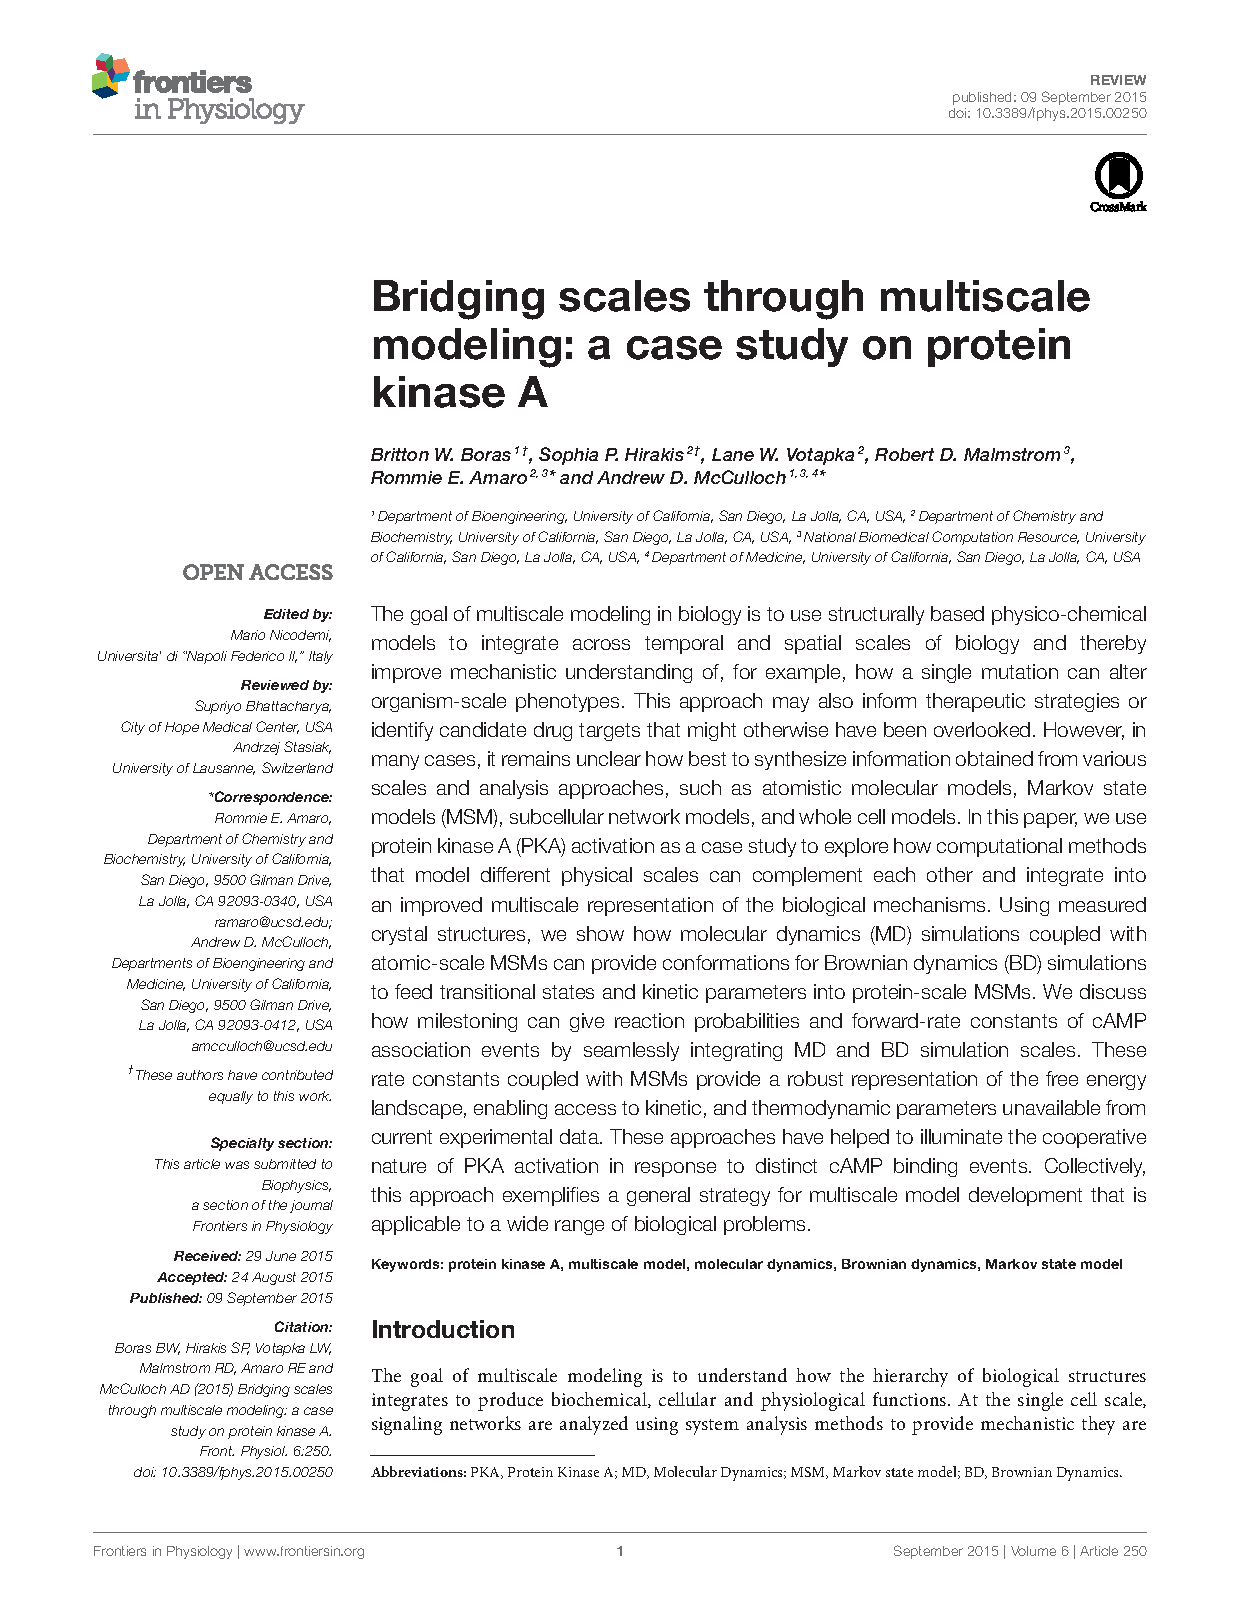
\includegraphics[height=0.82\textheight]{Frontiers_Paper_Chapter2.pdf}
In the following manuscript, we demonstrate ways in which multiscale computational methods can integrate structural and chemical information to better understand how, for example, changes in protein sequence such as point mutations can alter organ-level phenotypes like cardiac contraction. Our case study is focused on Protein Kinase A (PKA) and the manuscript provides examples of multiscale methods that compliment each other, showing how structural and kinetic information can be combined into an integrated understanding of the protein system. Included in the manuscripts are examples of how multiple short molecular dynamics (MD) simulations can be combined into an atomistic Markov State Model (MSM) to provide mechanistic insights and kinetic information about important structural transitions in the cyclic nucleotide binding domain (CBD) of PKA. Moreover, classical and accelerated  MD simulations can provide new structures to understand the association kinetics of the second messenger, cAMP using Brownian dynamics (BD) simulations. A complete description of this method is provided in Chapter 3 of the dissertation. BD simulations yield kinetic rates of bimolecular association reactions that can be used in protein-scale MSMs. An example of integrating BD with protein-level MSMs will be shown in Chapter 4 with a different protein system. Semi-analogous to MSMs are milestoning methods that have been developed and optimized by the Amaro lab to directly integrate MD and BD to understand on and off-rates of ligands to their protein systems. Finally, we discuss how the information provided by the aforementioned methods can be used in sub-cellular and whole cell models. 




%% Inserting the rest of the Fronteirs paper pages and add entries to LoF, LoT
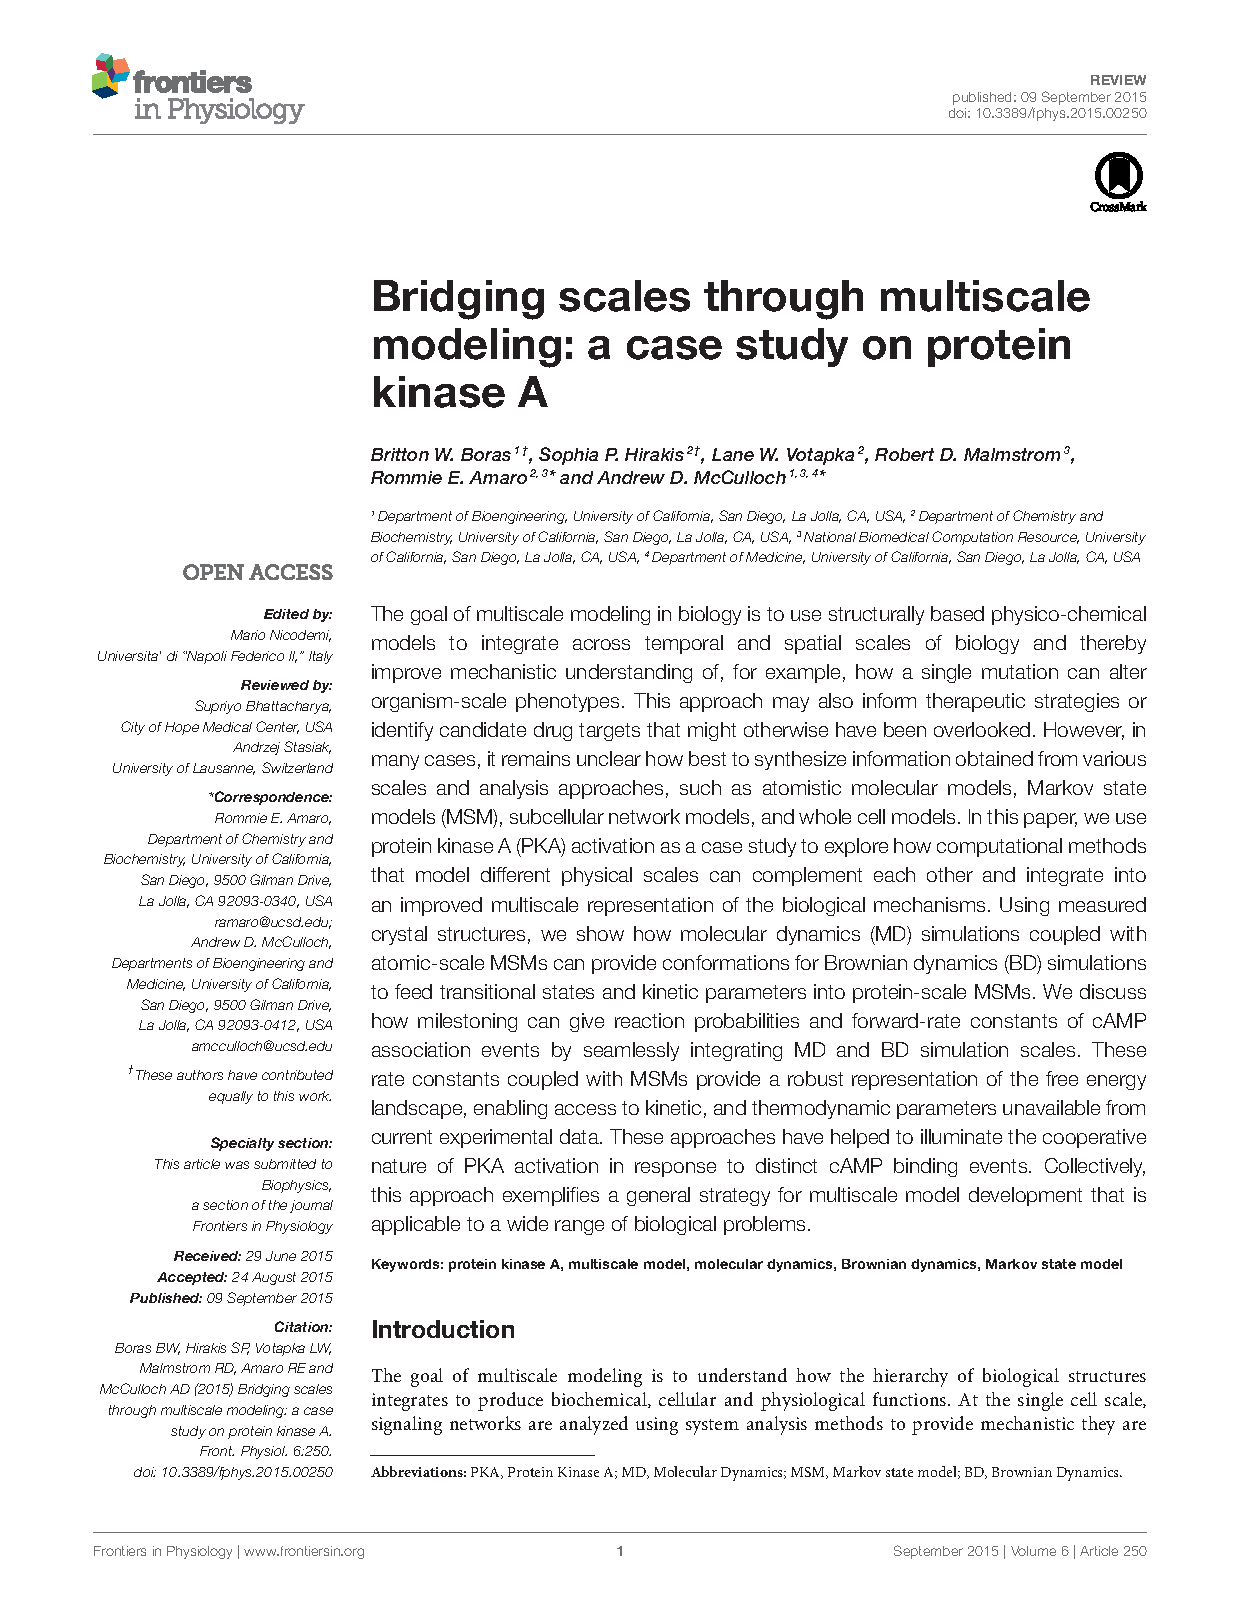
\includepdf[
  pages={-}, %% All subsequent pages
  scale=0.9,
  pagecommand={\pagestyle{myheadings}}, %% If you want to apply normal headers/footers
  %% Add to LoF and LoT. Note that the page numbers MUST be sorted.
  %  Page numbers here are _relative_ to the included PDF file itself.
  addtolist={
    2,figure, {Bridging gaps through multiscale modeling},fig:bridginggaps,
    3,scheme, {Activation Mechanism of PKA RI$\alpha$ with Different R conformations and Relative Association Rates}, fig:wide,
    4,figure, {Protein Kinase A cyclic nucleotide binding domain Markov state model}, figure:pkacbdmsm,
    6,figure, {Brownian dynamics simulation method}, figure:bd,
    8,figure, {Milestoning applied to unite MD and BD}, figure:MDBDmilestoning,
    10,figure, {The Markov State Model of PKA-RI$\alpha$ R$_{2}$C$_{2}$ holoenzyme}, figure:milestoning
%    3,scheme, {Activation Mechanism of PKA RI$\alpha$ with Different R conformations and Relative Association Rates}, fig:wide,
  }]{Frontiers_Paper_Chapter2.pdf} %%PDF to insert

\section{Acknowledgment}
This work was the result of a direct collaboration with wonderful co-authors whom I would like to formally acknowledge. Dr. Britton W. Boras, is the co-first author who wrote a portion of the paper and created figures used in the manuscript. Dr. Lane W. Votapka and Dr. Robert D. Malmstrom also wrote sections of the paper and helped to construct figures. Dr. Rommie E. Amaro and Dr. Andrew D. McCulloch provided support for the manuscript through editing and revision of the text. I extend my gratitude to the above-mentioned scientists for their creative and scientific contributions to the manuscript. 


%End of Chapter 1

%~~~~~~~~~~~~~~~~~~~~~~~~~~~~~~~~~~~~~~~~~~~~~~~~~~~~~~~~~~~~~~~~~~~~~~~
%Beginning of Chapter 2
\chapter{Visualizing and understanding protein-protein interactions with Molecular Dynamics}\label{cosmo_paper}
\vspace*{-1cm}
The following manuscript demonstrates the ways that protein-protein contacts involved in bacterial infectious mechanisms can be elucidated by protein crystallography and further understood using MD simulations. The subject of the manuscript, Group A \textit{Streptococcus} (GAS), is incredibly infectious with a wide range of symptoms ranging from sore throat to flesh-eating bacteria that affects the skin and internal organs such as the heart. Development of a vaccine treatment for GAS has been slow due to the large variance in sequence of its surface antigen M protein. Over 200 different types of M proteins have been identified and antibodies typically recognize only the hypervariable region (HVR) of the M protein, offering narrow specificity. The infectious mechanism of the protein is quite remarkable, as the Human C4b-binding protein (C4BP) interacts with around 90\% of M proteins, making it a great candidate for understanding the broad specificity of the HVR. In this study, crystal structures of C4BP in complex with four different M-proteins reveal the uniform and sequence-variant "tolerant" reading head of the protein-protein complex. 

In context of the thesis, this manuscript demonstrates how observations made by crystallographic methods are enhanced by molecular simulation. The MD study in this manuscript allowed us to visualize and understanding of the atomistic contacts which could not be explained by the static structure itself.
A number of mutants of the WT were which strengthened and weakened the contacts of the M protein-C4BP complex  Most notably, the MD showed how water is able to penetrate the protein complex due to a point mutation of a hydrophobic reside and how charged reside mutations counter-intuitively strengthen the interactions between C4BP and M protein complexes.   \\

\newpage
\includegraphics[height=0.79\textheight]{Buffalo_MainText.pdf}
\includepdf[
	pages={2-},
	scale=0.9,
	pagecommand={\pagestyle{myheadings}},
	addtolist={
    15,figure, {Structures of M-C4BP complexes},fig:C4BPstructures,
    16,figure, {C4BP Binding Mode},fig:bindingmode,
    17,figure, {C4BP-binding modes of M proteins},fig:mproteinbindingmode,
    18,figure, {M2-C4BP interaction},fig:interaction,
    19,figure, {Schematic of M protein domains},fig:domains,
    20,figure, {Electron density for the M49 HVR-C4BP$\alpha$1-2 complex},fig:electrondensity,
    21,figure, {Structure of M22-C4BP},fig:m22structure,
    22,figure, {Structure of M28-C4BP},fig:m28structure,
    23,figure, {Structure of M49-C4BP},fig:m49structure,
    24,figure, {Coiled coil parameters of M proteins},fig:coilcoil,
    25,figure, {Rotation of C4BP$\alpha$1-2},fig:rotation,
    26,figure, {Structure of the M22-C4BP interaction in which C4BP$\alpha$1 is tilted rather than rotated},fig:tilt,
    27,figure, {Sequence alignment of C4BP-binding M protein HVRs of the M2/M49 pattern},fig:alignmentM2M49,
    28,figure, {Sequence alignment of C4BP-binding M protein HVRs of the M22/M28 pattern},fig:alignmentM22M28,
    29,figure, {C4BP-binding M protein HVRs that cannot be classified as belonging to either M2/M49 or M22/M28 patterns},fig:hvr,
    30,figure, {C4BP-M2 interaction},fig:interactions,
    31,figure, {Molecular dynamics simulation of the Arg39 ‘hydrophobic nook’ interaction with wild-type M2 and M2 F75A},fig:MD,
    32,figure, {Interactions of M2 and M2 (K65A/N66A) with C4BP$\alpha$2},fig:interactions2,
    33,figure, {B-factors of C4BP$\alpha$2 bound to M2 or M2 (K65A/ N66A)},fig:bfactor,
    34,figure, {Uncropped Gels},fig:gels,
    35,table, {Data collection, phasing and refinement statistics for native and SAD (SeMet) structures},table:crystal,
    36,table, {Ionic Interaction Pair Occupancy in C4BP$\alpha$2 for Quadrilateral Residues of M2},table:occupancy1,
    36,table, {Ionic Interaction Pair Occupancy in Quadrilateral for Residues of M49, M22, and M28},table:occupancy2
  	}
 ]{Buffalo_MainText.pdf}


\section{Acknowledgment}
This work was the result of a direct and indirect collaboration with a collection of scientists whom I would like to acknowledge. My dear friend and colleague, Dr. Cosmo Z. Buffalo and I began our computational investigations of the M-proteins in complex with Human C4BP, albeit without the blessing of our advisors. He is responsible for the crystallographic characterization of the four complexes as well and wrote the manuscript. Adrian J. Bahn-Suh is Cosmo's student who also assisted with the experimental components of the work and figures. Dr. Tapan Biswas, a scientist on the project, assisted Cosmo in the refinement of the structures. My beloved advisor, Dr. Rommie E. Amaro, advised me on the data analysis and helped to write and revise the manuscript. Though not an author on the paper, Pek Ieong, a former scientist in the Amaro lab, provided invaluable advice for the analysis of the binding regions through fingerprinting algorithms that she developed using Kepler software. Dr. Victor Nizet and Dr. Patho Ghosh helped write the manuscript and advised on scientific studies to further refine the work. I thank them all humbly for welcoming my computational insights and for allowing me to collaborate on this wonderful project. 

%~~~~~~~~~~~~~~~~~~~~~~~~~~~~~~~~~~~~~~~~~~~~~~~~~~~~~~~~~~~
%Beginning of Chapter 3
\chapter{Bridging structural and mechanistic observations with computational modeling techniques}\label{first:paper}
\vspace*{-1.2cm}
In the following manuscript, we demonstrate how two distinct scales of molecular simulations can be used to understand the structure of a protein complex and suggest paths for the activation mechanism by a small molecule regulator. The subject of the manuscript is the heterotetrameric complex of Protein Kinase A (PKA), a ubiquitous eukaryotic protein responsible for turning proteins on and off in response to an extra-cellular stimulus. PKA is comprised of two catalytic (C) subunits that phosphorylate protein targets and regulatory (R) subunits (R$_{2}$C$_{2}$), each with two Cyclic-nucleotide binding Domains (CBD) named A and B, which bind a total of four equivalents of cAMP for each R dimer, thereby activating the two C subunits. The holoenzyme structure has been the subject of some controversy. Specifically, the interface between the Type 1A R and C subunit has been debated extensively by those in the PKA community. Solution-structure methodologies such as small-angle X-ray scattering (SAXS) and Hydrogen/Deuterium exchange Mass Spectrometry (H/DxMS) suggest a protein-protein interface that involves CBD-A. Crystallography of the full-length R in the holoenzyme complex proved challenging for the wild-type PKA, but a CBD-B mutant of R described a more-extensive interface that involved both CBD-A and CBD-B, observations that are inconsistent with the structural data already described.  

In this manuscript, MD simulations helped bridge the gap between the crystallographic and solution structures, revealing a stable conformation of the R subunit that was elucidated after only a few nanoseconds of simulations starting from the extended conformation of the R subunit in the crystal structure. In the wild-type form, the R subunit relaxes into a conformation which we named the Flipback conformation. With the new R subunit structure, a model of the heterotetramer was constructed and proved extremely consistent with the solution structure description. More specifically, the Flipback structure is consistent with solvent-exposure of the C subunit determined by H/DxMS and the shape of the molecule as suggested by SAXS. 

With this new  model of the heterotetramer, we decided to use Brownian Dynamics (BD) to investigate the differential association kinetics of the small-molecule regulator cAMP to the two proposed structures: 1) the (Holo) holoenzyme model derived from two crystal structures and 2) the Flipback model derived from our simulations and based on a crystal structure model. Before our experiments, it was known that cAMP preferentially binds to CBD-B and this was confirmed by our BD simulations.  What was revealed by our BD simulations was the association to the A-domain of the R subunit. In the heterotetrameric Flipback conformation, the association of cAMP to CBD-A was two orders of magnitude higher than to CBD-A of the crystallographic "Holo"  model. In the heterodimeric forms, the association difference was more pronounced, with four orders of magnitude higher association rates to the Flipback conformation over the Holo conformation. The difference in association kinetics is due to a re-distribution of the electrostatic charges as a result of the conformational differences. The electrostatic potential on the surface of the protein is responsible for the to the long-range attractive forces guiding the cAMP molecule to the CBD target. These findings suggest that the R subunit may adopt the Flipback conformation in order to bind cAMP in the A domain of PKA.

With these new insights from computational simulations, we have a better understanding of the heterotetrameric structure of PKA, bridging the gap between solution and crystallographic observations. Additionally, we predict the structure that PKA uses for the final step of activation-the association to CBD-A.   \\
%% Inserting the first page of the  Flipback paper as an image
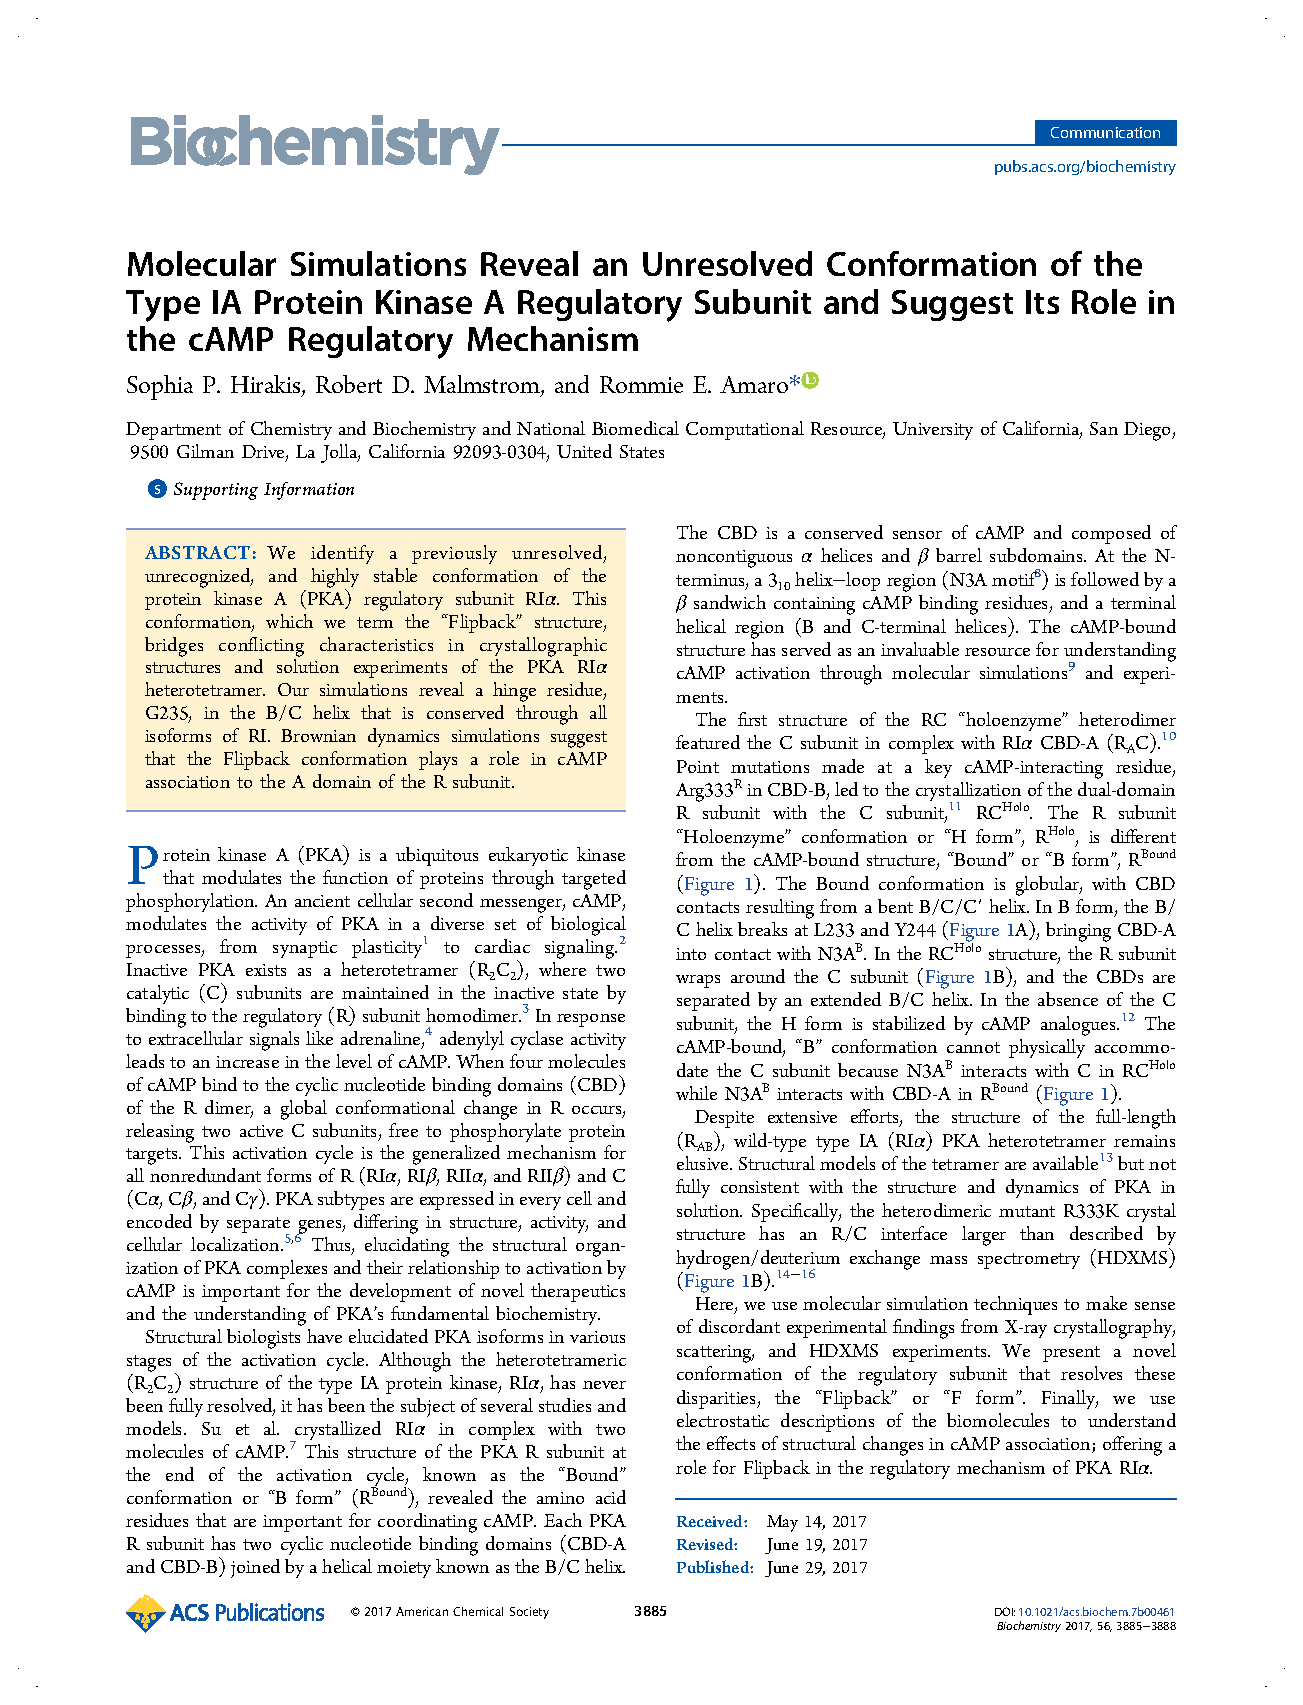
\includegraphics[height=0.9\textheight]{Flipback_Paper_Chapter3.pdf}

%% Inserting the rest of the Flipback paper pages and add entries to LoF, LoT
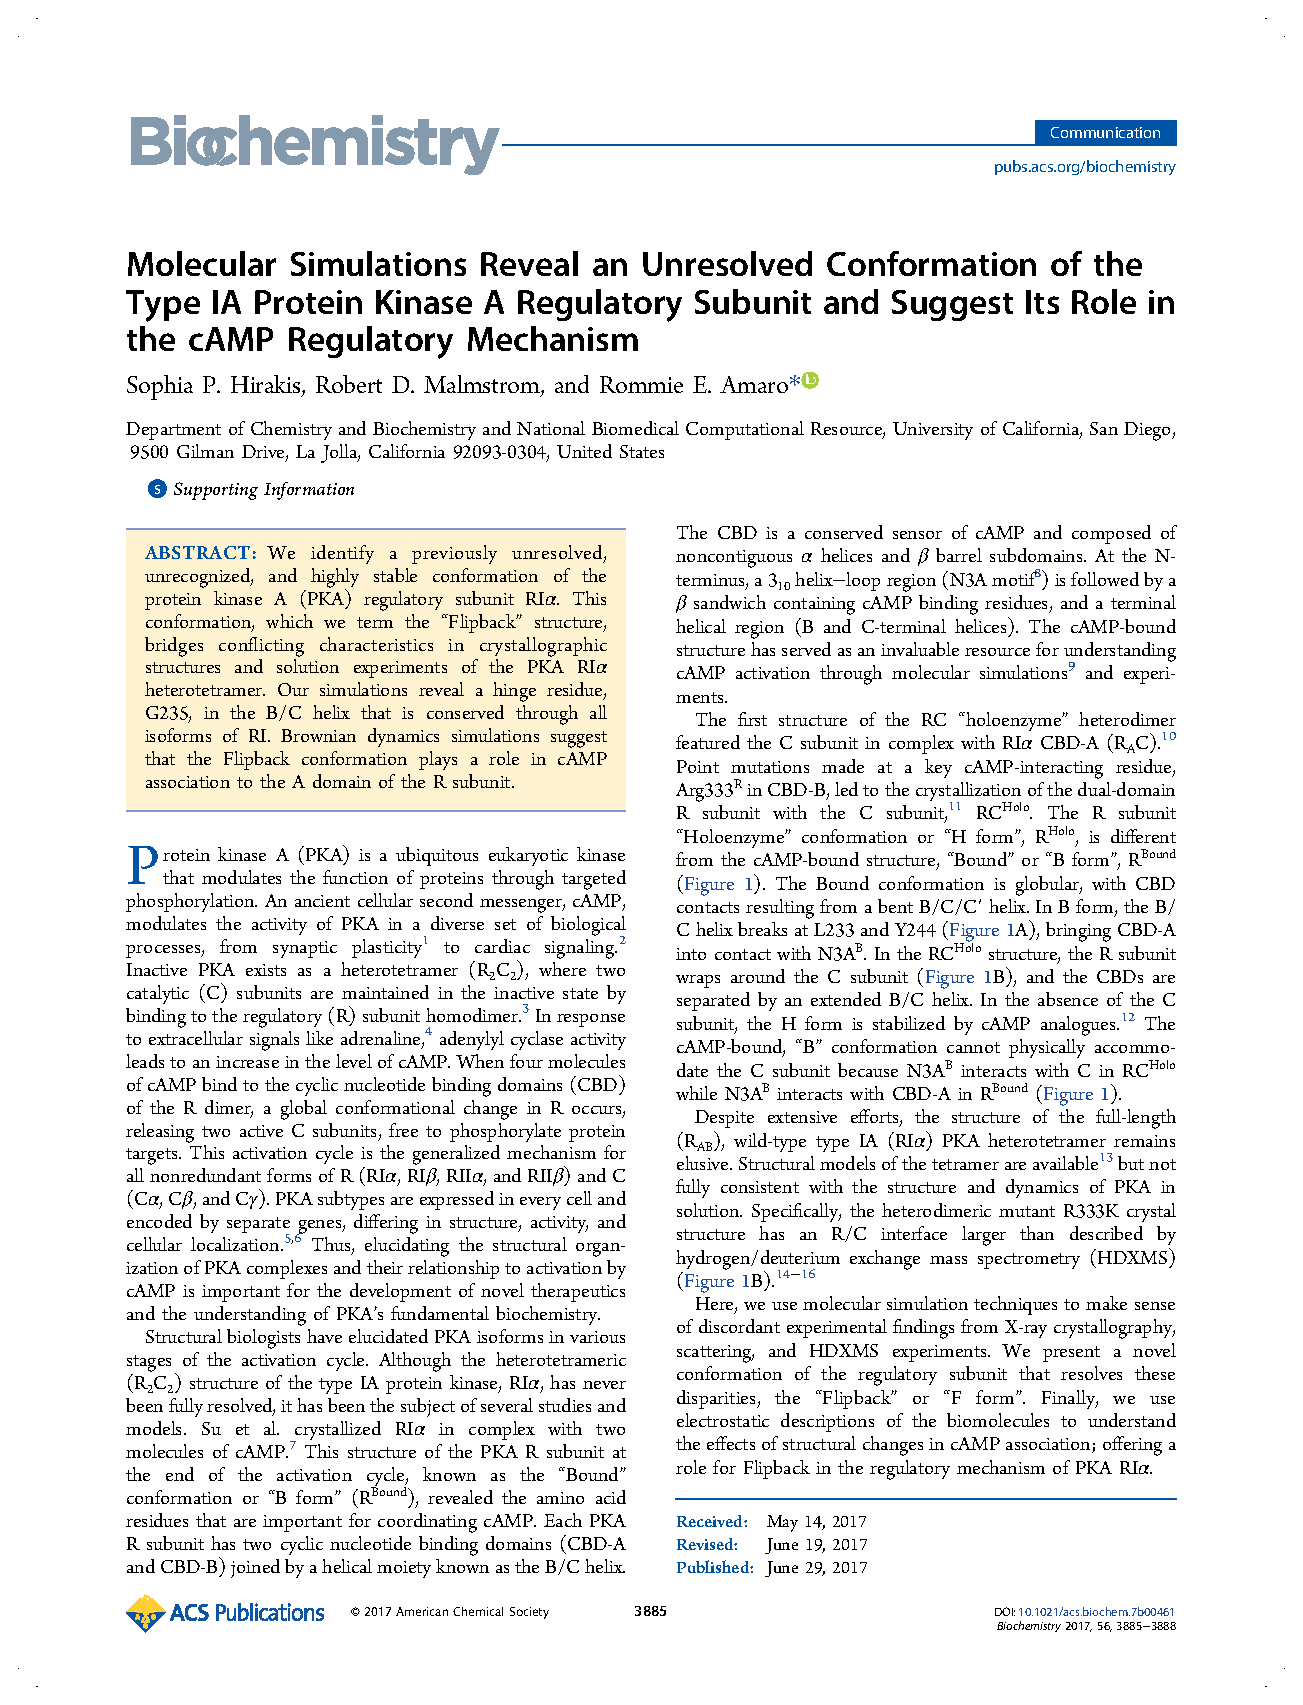
\includepdf[
  pages={2-}, %% All subsequent pages
  scale=0.9,
  pagecommand={\pagestyle{myheadings}}, %% If you want to apply normal headers/footers
  %% Add to LoF and LoT. Note that the page numbers MUST be sorted.
  %% Page numbers here are _relative_ to the included PDF file itself.
  addtolist={
    3,figure, {Comparison of the novel Flipback heterodimer with resolved PKA RI$\alpha$  Conformations},fig:comparison,
    2,table, {Rates of Association if cAMP with Cyclic Nucleotide Binding Domains of PKA complexes}, table:rates
  }
 ]{Flipback_Paper_Chapter3.pdf} %%PDF to insert



%% Inserting the first page of the  Flipback supplemental paper as an image
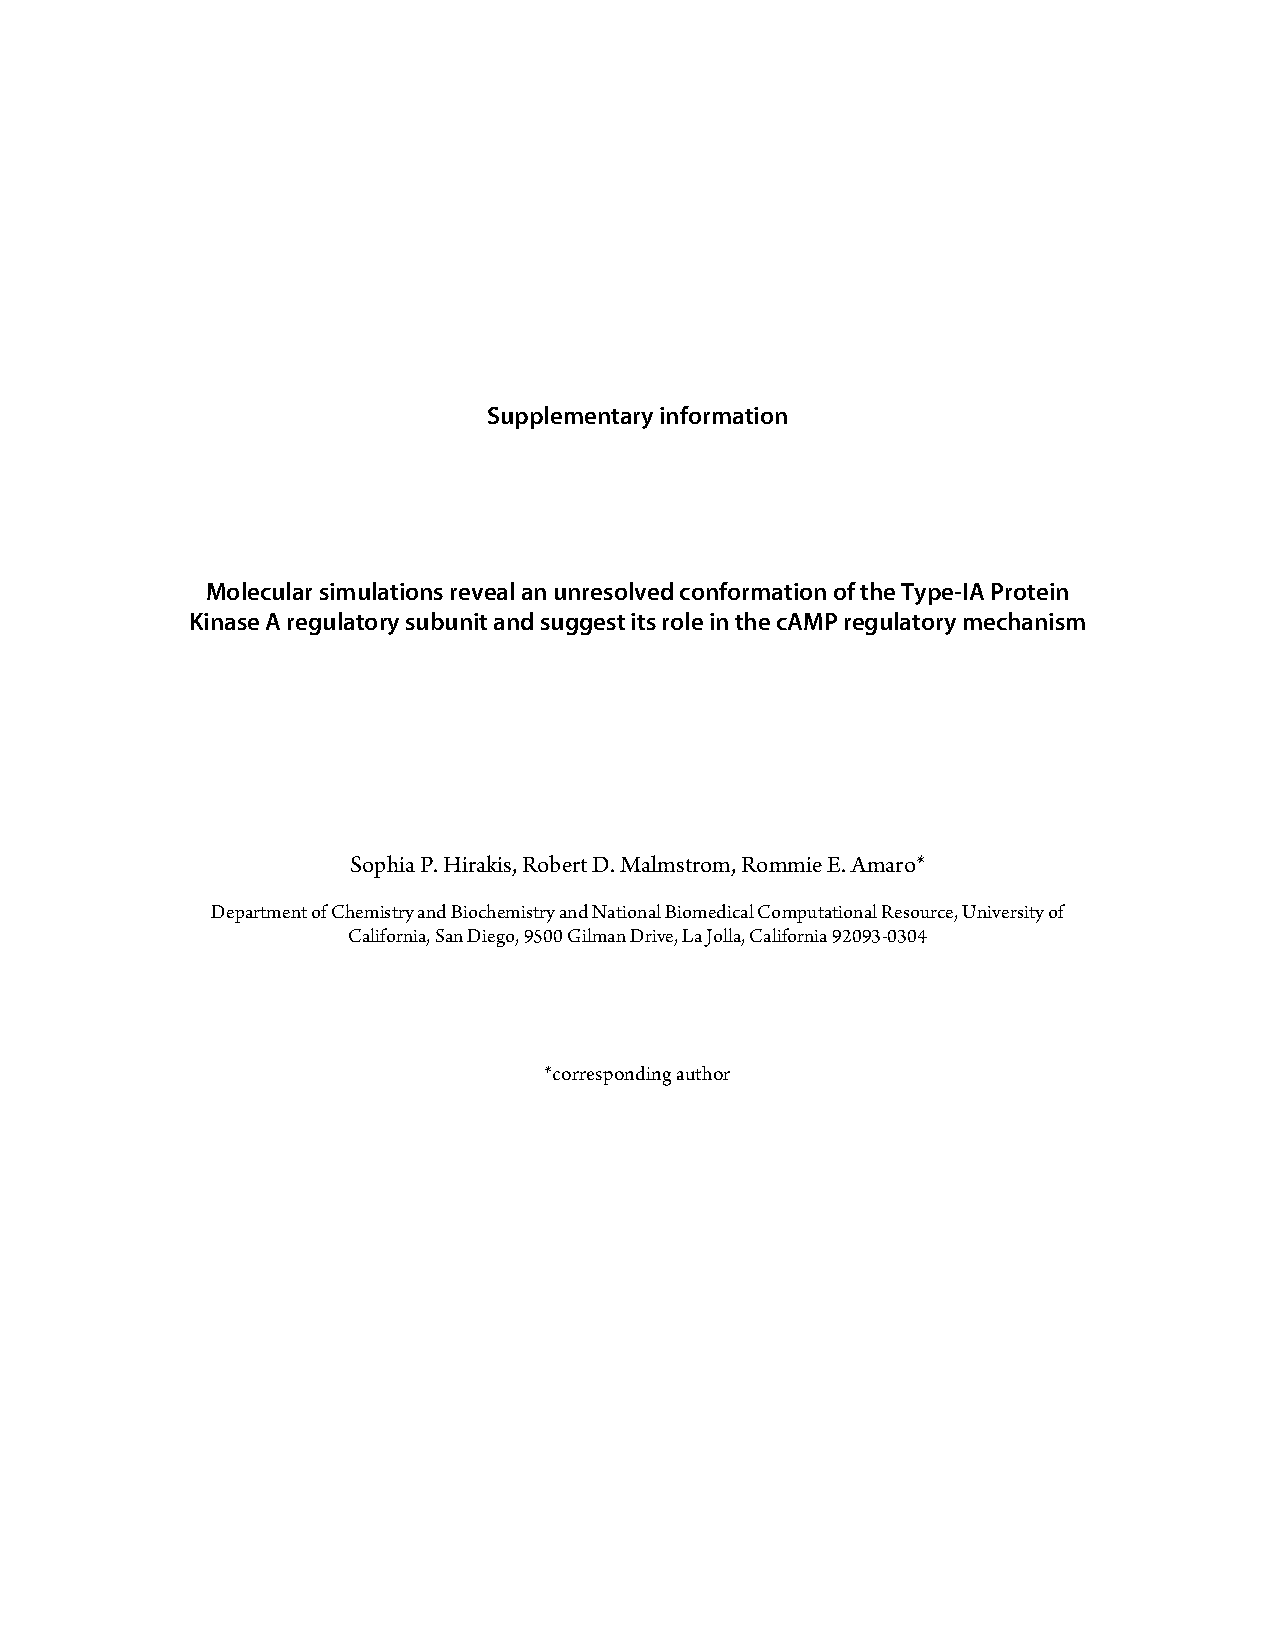
\includegraphics[height=0.8\textheight]{Flipback_Supplemental_Chapter3.pdf}

%% Inserting the rest of the Flipback paper pages and add entries to LoF, LoT
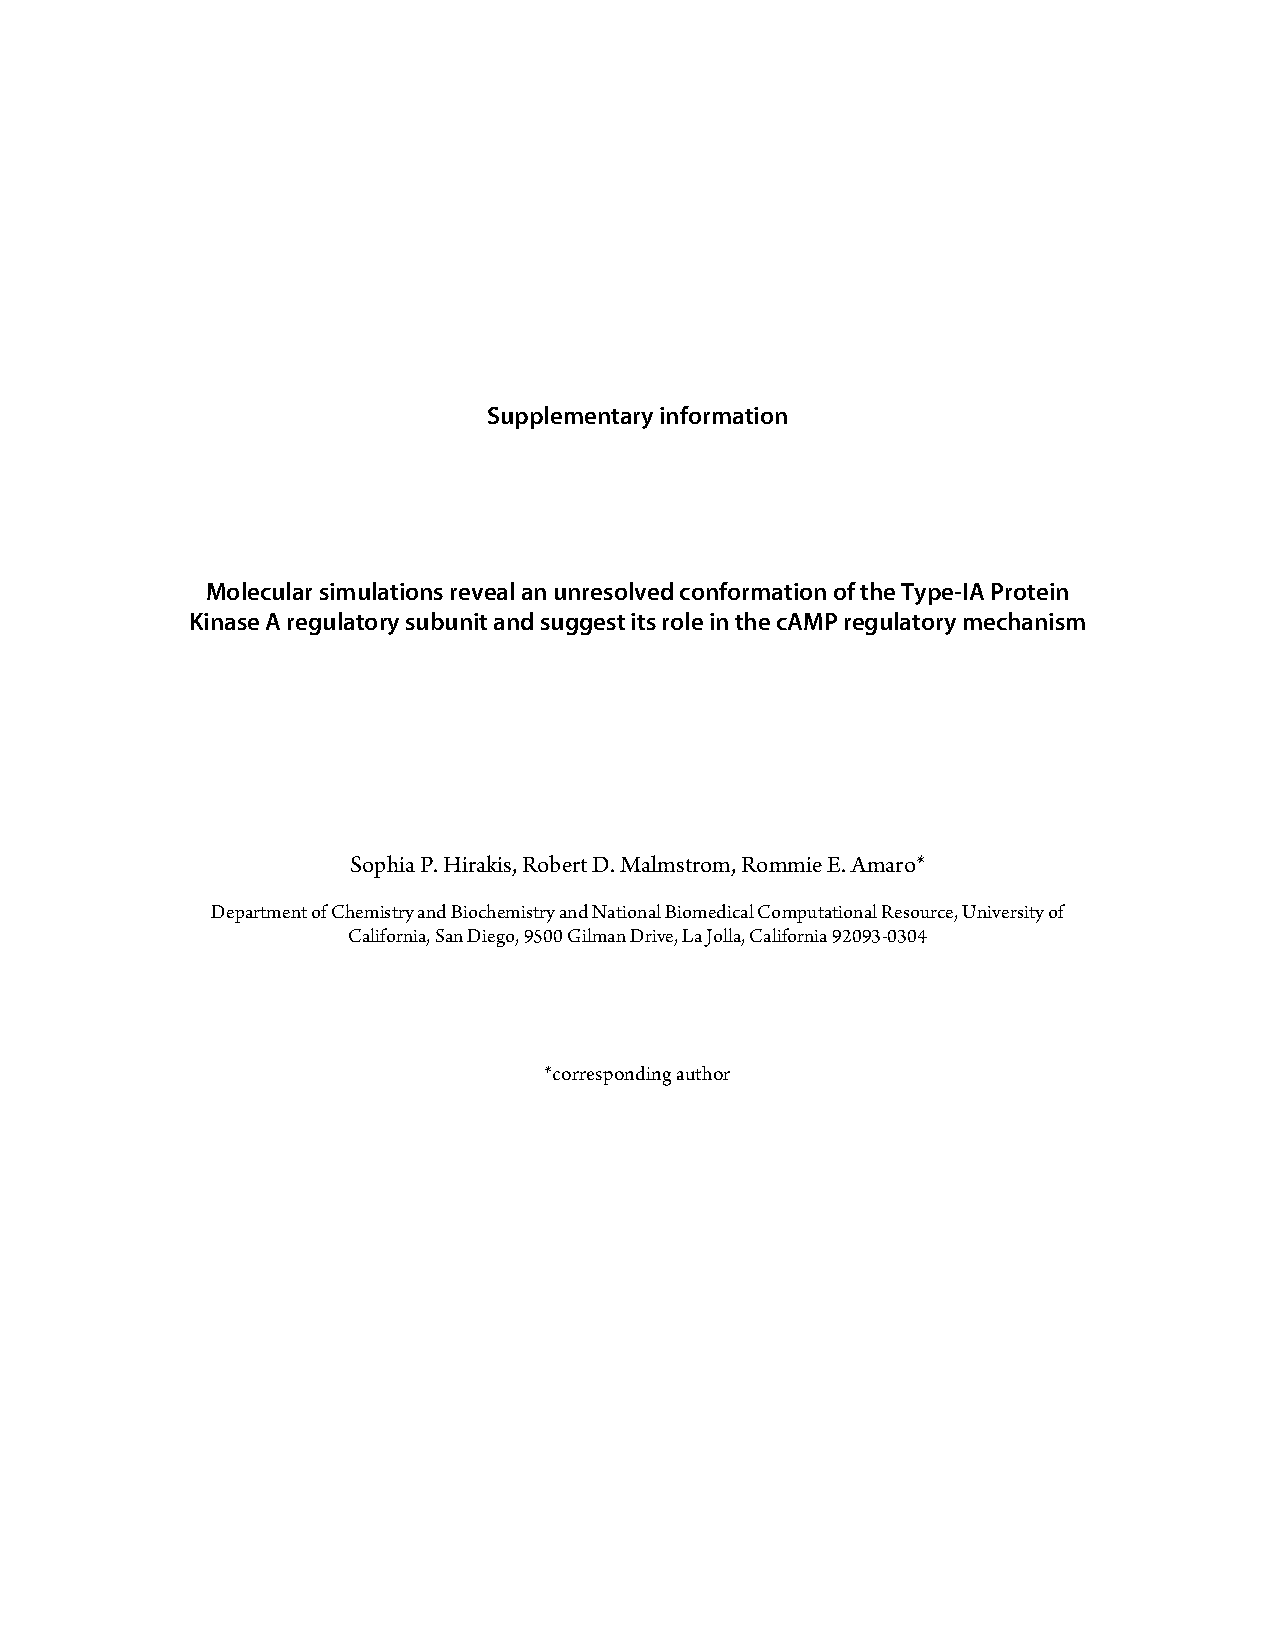
\includepdf[
  pages={2-}, %% All subsequent pages
  scale=0.9,
  pagecommand={\pagestyle{myheadings}}, %% If you want to apply normal headers/footers
  %% Add to LoF and LoT. Note that the page numbers MUST be sorted.
  %% Page numbers here are _relative_ to the included PDF file itself.
  addtolist={
    3,figure, {The stability of the Flipback conformation},fig:stableflipback,
    4,figure, {Generalized encounter compled of cAMP and the CBD-A/B},fig:encountercomplex,
    4,table, {Encounter Complex Description of R subunit and cAMP},table:rates,
    4,figure, {Atomic numbering and naming of cAMP molecule in BD simulations},fig:cAMPnumbers,
    5,figure, {Electrostatic descriptions of the four systems},table:rates
  }
]{Flipback_Supplemental_Chapter3.pdf} %%PDF to insert



\section{Acknowledgment}
This discovery would not have been possible without the original simulations by Dr. Robert D. Malmstrom. Dr. Malmstrom allowed me to analyze his simulations and through this, I discovered the Flipback conformation. Dr. Malmstrom assisted in the manuscript review. Though not listed as an author, special thanks goes out to Dr. Alexandr Kornev who assisted in the understanding of the Flipback conformation in the context of the existing literature on PKA heterotetramer. He provided critical edits to the document which helped project it towards success and acceptance in the field. Dr. Susan S. Taylor provided insights and I thank her for the many conversations about this. Dr. Lane W. Votapka and Dr. Gary Huber assisted with the construction of the BrownDye simulations and for this, I thank them. Dr. Jamie M. Schiffer helped understand the SAXS profiles of PKA tetramer. Dr. Elizabeth Komives provided support for the discovery of the structure and much welcomed enthusiasm for the publication of the manuscript. Finally, I thank my beloved advisor, Dr. Rommie E. Amaro for pushing me to publish this work and for helping me to see the value in my findings, which the world may never have known of if not for her invaluable encouragement. Thus, cardiac function spans multiple scales of space and time, from that which can be seen with the naked eye, to that which only a computational microscope can observe.

%End of Chapter 3

%~~~~~~~~~~~~~~~~~~~~~~~~~~~~~~~~~~~~~~~~~~~~~~~~~~~~~~~~~~~~~~~~~~~~~~~

%Beginning of Chapter 4


%...
\chapter{Subcellular spatial modeling in realistic geometries with stochastic particle methods to understand heart disease}

\section{Introduction}
The actor playing a major role in the underlying mechanisms of the heartbeat is \textit{smaller than you think}. Over 135 years ago, Dr. Singer demonstrated that a human heart would not beat in the absence of Ca\textsuperscript{2+} \cite{Ringer1883}. As a process, the heartbeat is an inherently multiscale process. The human heart is about the size of a human fist. The atria and ventricles of the heart make up the "working chambers" which pump oxygenated blood through the body, and deliver deoxygenated blood to the lungs. The thickness of these walls are several millimeters depending on the region of the heart. Each cell is a complicated but regular structure of membranous invaginations that range from 20-450 nm in diameter. Cardiomyocytes, or muscle cells, contain bundles of muscle fibers that are responsible for the contraction of the heart. The thick filaments are made out of myosin protein and are about that are 160-170 \si{angstrom} in diameter while thinner actin filaments are 6 to 10\si{angstrom} in diameter. Finally, large proteins in close contact with each other, (roughly 20 nm) sense calcium ions (roughly 231 pm radius) triggering processes that result in the beating of the heart. Thus, cardiac function spans scales that can be observed with the naked eye, to invisible phenomena that only a computational microscope can see.  

 A healthy heart contracts in response to a synchronous electrical stimulation of the plasma membrane, also known as the sarcolemma, initiated by the sinoatrial (SA) node. The membrane action potential travels from the SA node and is propagated from cell to cell through gap junctions\cite{Bernstein2006}. This electrical stimulation results in membrane depolarization, to which the cell responds with a muscular contraction, a phenomenon known as  excitation-contraction coupling (ECC)\cite{Cheng1994}. 
 
 Cardiomyocytes have specialized structures within which this process occurs. Invaginations in the sarcolemma (cell membrane), known as axial and transverse-tubules (TT) are positioned directly adjacent to the sarcoplasmic reticulum (SR), the intracellular calcium store. Depolarization of the sarcolemma activates and opens L-Type Calcium Channels (LTCC), through which calcium enters the cell. The LTCC are in close proximity large ($>2$MDa) SR membrane proteins called Ryanodine Receptors (RyR) \cite{Lanner2010}. The space between the extracellular membrane and SR membrane is known as the dyadic junction and \textit{this is where the magic happens}.

High calcium concentrations in the extracellular matrix cause influx of Ca\textsuperscript{2+} through LTCC, into the cardiac muscle cells which maintain a very low Ca\textsuperscript{2+}  concentration. Directly adjacent to LTCC, RyR, regulated by more than 30 proteins\cite{Fill2002}, cause a \textit{signal amplification} by releasing thousands of Ca\textsuperscript{2+}  ions from the SR into the cell, an event known as a triggered calcium spark. In response to the high increase in the second-messenger, Troponin C (TnC) molecules bind Ca\textsuperscript{2+}, relieving the inhibition of actin on myosin. These muscle fiber proteins slide across each other leading to muscle fiber shortening, or muscular contraction that squeezes blood out of the atrial chambers of the heart into the ventricles and out towards the rest of the body. 

Early on, LTCC (also known as Dihydropyridine Receptors, and Voltage-Dependent Calcium Channels) \cite{Lu1994} and RyR \cite{Stern1999} were implicated in the generation of calcium sparks. Though theories about ECC existed \cite{Stern1992}, the first Ca\textsuperscript{2+} spark event was visualized and confirmed 25 years ago using laser-scanning confocal microscopy \cite{Cheng1993} and quickly confirmed in subsequent studies \cite{Cannell1994,Cannell1995}. Within a few years, computer simulations were applied to this system to model the elementary events responsible to elucidate the subcellular mechanisms responsible for what was visualized with the early fluorescence measurements \cite{Cannell1997}. 

Imaging techniques have limitations in terms of their ability to resolve spatial changes in calcium levels. Therefore, computational models have played an important role to tease out important features of CICR and ECC \cite{Maleckar2017}. The field has an impressive track-record of over 30 years of computational modeling of cardiac excitation phenomena. 

In 2012, Hake et al. debuted the first subcellular model of a Calcium spark \cite{Hake2012} using realistic geometries of a cardiac calcium unit \cite{Hayashi2009}.  In this study, we combine the realistic geometries used by Hake et al. with stochastic models approaches using particle-based, spatial reaction-diffusion modeling methods.\cite{Hirakis2018}. We investigate the effects of disease phenotypes, such as T-Tubule deformation\cite{Louch2010}, RyR dispersion\cite{Kolstad2018}, and alterations of the mouse Action Potential\cite{Morotti2014} on calcium signaling. 


The first use of stochastic particle simulations to investigate cardiac Ca\textsuperscript{2+} signaling mechanisms was by Koh et al. in 2006\cite{Koh2006}. In their study model, Koh et al. showed the effects of altering dyadic volume had a pronounced effect on Ca\textsuperscript{2+} SR fluxes. In our study


 \section{Methods}
 
 \subsection{Building the Geometric Model}
 
 The our model aims to build upon and extend the first-built by Hake et al. \cite{Hake2012}, the first to use electron tomography-derived geometries for calcium spark simulations. We used the same realistic geometry of the calcium release unit (CRU) imaged by Hayashi et al. \cite{Hayashi2009} which were segmented by IMOD \cite{Mastronarde2008} and meshed with GAMer \cite{Yu2008}. The geometry files were graciously provided to us through correspondence with Johan Hake, the primary author of the CRU paper \cite{Hake2012}. We were also very fortunate to have access to the original EM images through the local National Computational Microscopy Imaging Resource (NCMIR) at UCSD. Although the original segmented images did not include the explicit locations of the Ryanodine Receptors (RyR) in the junctional SR, images of the locations were graciously provided to us by Masahiko Hoshijima of NCMIR. In total, 96 RyR were observed in the original CRU tomograms and this number of RyR were used in our simulations.
 
The features a contiguous sarcoplasmic reticulum (SR), two mitochondria, and one axial and one transverse tubule (TT1 and TT2 respectively). In order for the geometry mush to be usable by our simulation interface and simulation engine, (CellBlender and MCell) it was necessary to further refine the mesh. For this, we used an improved version of GAMer developed locally at the National Biomedical Computational Resource (NBCR) at UC San Diego (UCSD) \cite{Yu2008,Lee2018}.

To divide the mesh into "model objects" usable by MCell and Cellblender, we used the colors attributed to the original meshes as a way to classify the objects into separate regions. The model objects were named as follows: 1) T-Tubule 1 (TT1, axial); 2) T-Tubule 2 (TT2, transverse); 3) Mitochondrion 1 (Mito1); 4) Mitochondrion 2 (Mito2); 5) Sarcoplasmic Reticulum (SR). The SR was further subdivided into network SR, Z-line SR, and junctional SR subdivided in the following ways: a) nSR1, nSR2, nSR3, nSR4, nSR5, nSR6; b) SRZ1, SRZ2; c) jSR release site, jSR rim, jSR back.

In diseased states, T-Tubule networks are known to be disrupted \cite{Louch2010,Ibrahim2011,Crossman2015}, which oftentimes results in increased dyadic junction distances \cite{Polakova2013}. In an effort to understand the effect that disease phenotypes have on calcium signaling, we deformed the (TT2) T-Tubule that interfaces with the junctional SR, in a way that did not significatly alter the volume or the surface area. The WT or "normal" T-Tubule and the "deformed" T-Tubule simulations were then compared against oneanother to understand the effects of the deformations in cardiac signaling. 

Although the number of calcium release units in a cardiac myocyte is on the 

\subsection{The MCell model of the CRU}
Our model uses a stochastic modeling engine named MCell \cite{Stiles2001a,Kerr2008,Czech2009} to track the positions of each molecule in the system individually. This approach treats molecules as points in space, able to diffuse in three dimensions of space. Reactions between species happen only when two molecules spatially encounter each other. Each molecule is accounted for explicitly in contrast to the continuum methods used by Hake et al. \cite{Hake2012}. 

The same cytosolic and SR $Ca^{2+}$ buffers were used in our MCell model; namely, ATP\cite{Bers2001,Picht2011,Hake2012}, Calmodulin (CMDN) \cite{Robertson1981,Fabiato1983,Michailova2002,Picht2011}, Troponin C (TRPN) \cite{Bondarenko2004}, and  Fluo-4 \cite{Picht2011} in the cytosol and Calsequestrin (CSQN)\cite{Shannon1997,Bers2001,Picht2011} and Fluo-5 in the SR \cite{Picht2011}. The models of the sarcolemmal (T-Tubule) pumps and SR pumps used by Hake et al. did not use elementary reactions, and so we used analogous models well-suited to model the behavior of the Plasma Membrane Calcium-ATPase (PMCA) \cite{Penheiter2003,Brini2009,Bartol2015}, Sodium-Calcium Exchanger (NCX) \cite{Hilgemann1991,Bartol2015}, Sarco/Endoplasmic Reticulum Calcium-ATPase (SERCA) pump\cite{Higgins2006,Bartol2015}, and (RyR)\cite{Saftenku2001}. The most important feature of these models is the ability to model the kinetics of individual calcium ions. Considerable adaptation of the models was necessary to achieve steady-state behavior in the absence of stimulus, which is detailed in the corresponding molecule descriptions below.

The CRU model of a $Ca^{2+}$ spark by Hake et al. \cite{Hake2012} was not designed to model the phenomenon known as Calcium Induced Calcium Release(CICR); an action potential-mediated excitation mechanism of L-Type Calcium Channel (LTCC) fluxes triggering $Ca^{2+}$ efflux from the SR through RyR channels. Instead, Hake's original model was used to understand spark termination. It utilized a phenomenological model of the Ryanodine Receptor that occupied one of two states, on or off. Ryanodine receptors were not activated in response to a particular signal, and the number of open receptors was set to a constant number. Moreover, the $Ca^{2+}$ signal terminated in response an SR $Ca^{2+}$ concentration pre-set by the model builders. We sought out to simulate CICR stochastically in response to sarcolemmal excitation. To do this, we implemented a Markov Model of RyR \cite{Saftenku2001} as well as model of the LTCC \cite{Greenstein2002} that features both voltage dependent and calcium dependent activation and inactivation properties. Effectively, our RyR respond dynamically to an calcium sparklet generated by LTCC openings in response to a membrane voltage change. Most importantly, our RyR are activated only by the spatial reaction of $Ca^{2+}$ with RyR.

\subsection{Experimental design}
One major difference between our model and the earlier model that used the same geometry \cite{Hake2012} is our use of stochastic simulations to understand Ca\textsuperscript{2+} spark dynamics in the CRU. Utilizing the power of MCell, we are able to count the exact positions and numbers of the molecules that comprise our system.  The molecules in our systems are modeled as particles that diffuse according to a specified molecular diffusion rate according to the equations of Brownian motion\cite{Stiles2001a}. The reactions in our systems can be unimolecular (state transitions) or bimolecular. Bimolecular reactions occur only upon spatial encounter,  and can happen between two cytosolically diffusing molecules (volume molecules) or with membrane-bound species (surface molecules). The Monte Carlo  algorithm used by MCell ensures that each simulation gives an independent result that is non-deterministic.

A second major difference between our model and Hake's CRU model is the use of an electrical stimulus to induce a Ca\textsuperscript{2+} spark. As noted earlier, the model by Hake et al. used a phenomenological discription of the RyR in the dyadic junction, whereby the number of RyR open was set to a constant. When set to open, RyR would "release" Ca\textsuperscript{2+} from the SR that is equivalent to a concentration gradient. Our model requires the use of an electrical stimulus to activate LTCC in the T-Tubules. Upon binding Ca\textsuperscript{2+} On the cytosolic side of the Ryanodine Receptor, individual  Ca\textsuperscript{2+} are released from the sarcoplasmic reticulum into the cytosol. With these improvements,We are able to investigate a multitude of questions that were not possible using the earlier model design.

With the use of stimulus-induced LTCC opening, we were able to investigate the effects of action potential alteration on calcium spark genesis. We accomplished this by using action potentials derived from healthy and diseased left ventricle myocytes. More specifically, we used a model of over-expressed Calmodulin-dependent Kinase II (CaMKII-OE) \cite{Morotti2014}
 

The use of the realistic geometry also lends the ability to understand the effects of morphological changes in the membranous structures. 

During the course of our investigations, we sought to understand the effects of 


\begin{comment}

\nocite{Louch2010}
\nocite{Valent2007}
\nocite{Bers2001}%
\nocite{Pitch2011}%
\nocite{Michailova2002}%
\nocite{Fabiato1983}%
\nocite{Robertson1981}%
\nocite{Bondarenko2004}
\nocite{Saftenku2001}%
\nocite{Guo2012}
\nocite{Greenstein2002}
\nocite{Brini2009} %
\nocite{Penheiter2003} %
\nocite{Hilgemann1991}%
\nocite{Higgins2006}%

\end{comment}


\subsection{Cytosolic and SR $Ca^{2+}$ Buffering}


The kinetics for our cytosolic and SR $Ca^{2+}$ buffers were modeled similarly to Hake et al (2012) according to equation 4.1. The cytosolic buffers in our simulations are ATP, Calmodulin (CMDN), Troponin-C (TRPN), and Fluo-4 and our SR buffers are Calsequestrin (CSQN) and Fluo-5.  The buffer reaction mechanism is a simple two-step reaction, where the buffer an exist in either apo or $Ca^{2+}$-bound states. 
\begin{equation}. 
\ce{B + Ca^2+  <=>[\ce{k_{f}}][\ce{k_{r}}]
$\underset{\text{Calcium-bound Buffer}}{\ce{B \cdot Ca^{2+}}}$
}
\end{equation}

At equilibrium, the product of the forward rate, k$_{f}$ and the concentration of $Ca^{2+}$  and the buffer is equal to to product of the concentration of the $Ca^{2+}$-bound buffer and the reverse rate, k$_{r}$, according to equation 4.2.  

\begin{equation}
k_{f}[B][Ca^{2+}] = k_{r}[B \cdot Ca^{2+}]
\end{equation}

At equilibrium, the concentration of $Ca^{2+}$ is assumed to be constant. In this way, we can assume a pseudo-first order rate, k, equaling to the product of the forward rate k$_{f}$ multiplied by the concentration of Calcium, according to equation 4.3. 
\begin{equation}
 k = k_{f} \cdot [Ca^2+]
\end{equation}

The pseudo-first order relationship in equation 4.3 can be substituted into equation 4.2, yielding equation 4.4.
\begin{equation}
k[B] = k_{r}[B \cdot Ca^{2+}]
\end{equation}

The above equation can be rearranged to give a ratio of the concentrations of the apo and Calcium-bound buffer state equaling to the ratio of the reverse and pseudo-first order rate.
\begin{equation}
\frac{[B]}{[B  \cdot Ca^{2+}]} = \frac{k_{r}}{k} 
\end{equation}

Since the buffer exists in either apo or calcium-bound states, according to equation 4.6, the relationship can be substituted into equation 4.5 solving for the concentration of the apo buffer species in 4.7. 
\begin{equation}
[Total_{B}] = [B] + [B \cdot Ca^{2+}] 
\end{equation}

\begin{equation}
\left[ B\right] = \frac {\left( \frac {k_{r}}{k}\right) \left [Total_{B}\right] }{ 1+\left( \frac {k_{r}}{k}\right) }
\end{equation}

Using this relationship, we are able to solve for the concentration of the buffer species in either apo or $Ca^{2+}$-bound states according to their total concentrations used by Hake et al. The values for the initial concentrations can be found in Table 4.1.
\subsection{Sarcolemmal (T-Tubule) Fluxes}

\subsubsection{PMCA and NCX fluxes}

There are two major sarcolemmal pumps known to maintain homeostasis in cardiomyocytes, the Plasma Membrane Calcium-ATPase (PMCA) pump and the Sodium-Calcium exchanger (NCX) pump \cite{Bers2002}. Hake et al. originally modeled the sarcolemmal pumps using three separatefluxes, PMCA (termed pCa in Hake et al.), NCX, and a background calcium flux, (termed Cab in Hake et al.). In our model, we capture the background calcium flux utilizing "leak" reactions in both our PMCA and NCX models (see Figure 4.1). 

\begin{figure}
\centering
	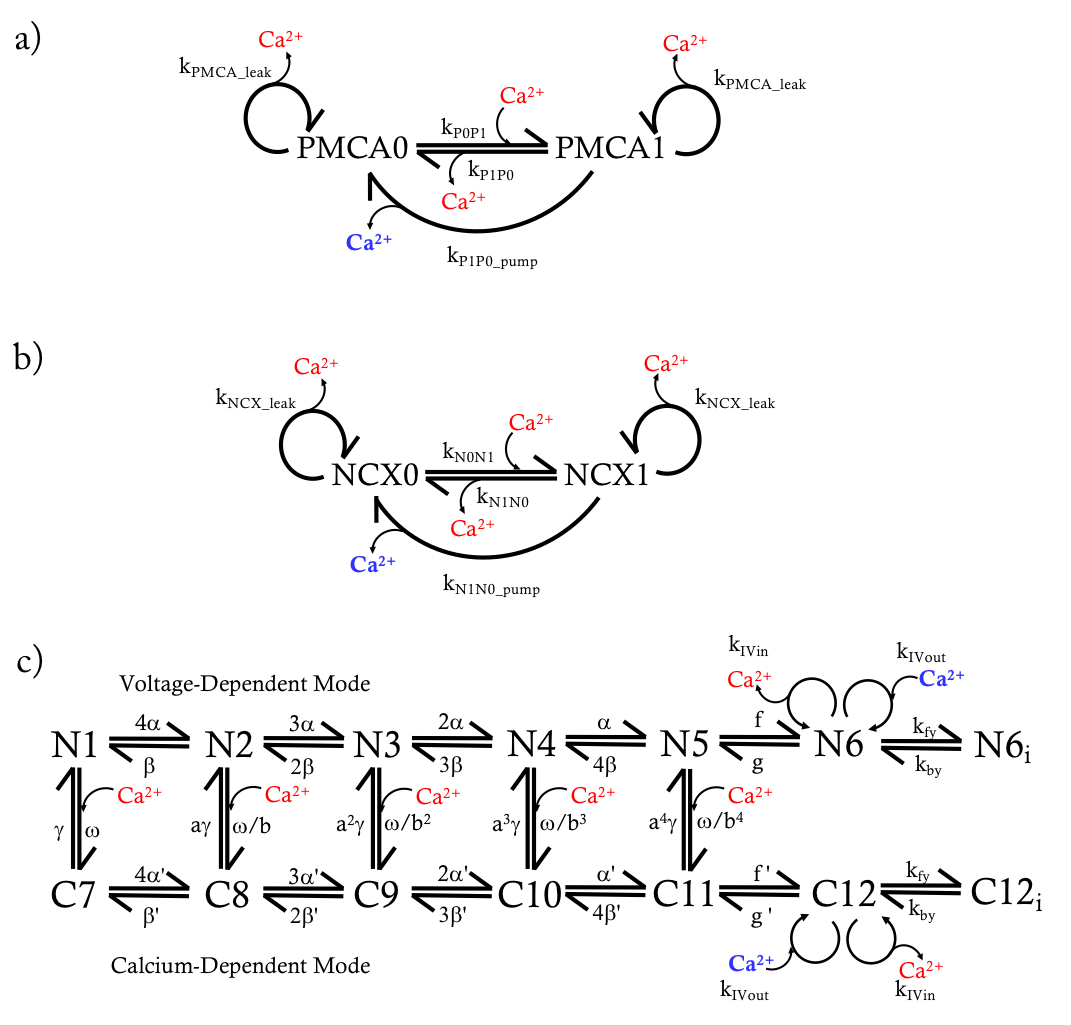
\includegraphics[scale=0.85]{TTfluxes_fig.png}
	\caption{Sarcolemmal (T-Tubule) Fluxes}
	\subcaption{Plasma Membrane Calcium-ATPase Model. Adapted from the model by Bartol et al. (2015) and based on measurements by Brini and Carafoli (2009) and Penheiter et al (2003). Both states are capable of leaking calcium into the cytoplasm (red), corresponding to a background calcium level of 140mM. The transition from state PMCA1 to state PMCA0 pumps one Calcium ion per reaction to the extracellular space (blue). Reaction rates can be found in Table 4.2;   \textbf{(b)} Sodium/Calcium Exchanger Model. Adapted from the model by Bartol et al. (2015) and based on measurements by Hilgemann (1991). Both states are capable of leaking calcium into the cytoplasm (red), corresponding to a background calcium level of 140mM.The transition from state NCX1 to state NCX0 pumps one Calcium ion per reaction to the extracellular space (blue). Reaction rates can be found in Table 4.2;   \textbf{(c)}Sodium/Calcium Exchanger Model. Adapted from the model by Bartol et al. (2015) and based on measurements by Hilgemann (1991). Both states are capable of leaking calcium into the cytoplasm (red), corresponding to a background calcium level of 140mM.The transition from state NCX1 to state NCX0 pumps one Calcium ion per reaction to the extracellular space (blue). Reaction rates can be found in Table 4.2 }
	
\label{fig:TTfluxes} 
\end{figure}

The PMCA pump is modeled as a two-state reaction where one ion of Ca$^{2+}$ can reversibly bind to the first state, and in a seperate, irreversible reaction, calcium is pumped out of the cytosol (see Figure 4.1a and equation 4.8). 
\begin{equation}
\ce{PMCA0 + Ca^2+  <=>[\ce{k_{1}}][\ce{k_{-1}}]
$\underset{\text{Calcium-bound Pump}}{\ce{PMCA1}}$
} \ch{ ->[pump] PMCA0}
\end{equation}

The concentration of either state is defined, then, by the total concentration minus the concentration of the other state, according to equation 4.8.

\begin{equation}
\left[PMCA_{1}\right] =\left[PMCA_{Total}\right] - \left[PMCA_{0}\right]
\end{equation}

At equilibrium the concentration of Ca$^{2+}$ is constant, and thus, a pseudo-first order rate, k$_{f}$, can be assumed, as in equation 4.10. 

\begin{equation}
k_{f} = [Ca^{2+}] \cdot k_{1}
\end{equation}

The rate of change of a state, for example, PMCA$_{0}$, can be written as the equation in 4.11, which is simply the sum of the rate of PMCA$_{0}$ producing reactions minus PMCA$_{0}$ consuming reactions.
\begin{equation}
\frac{d\left[PMCA_{0}\right]}{dt} = \left[PMCA_{1}\right]k_{-1} + \left[PMCA_{1}\right] k_{pump} - \left[PMCA_{0}\right] k_{f}
\end{equation}

At equilibrium, the rate of change is zero, and can be used to solve for the concentration of one of the two states as in equations 4.12-4.15.
\begin{equation}
0 = \frac{d\left[PMCA_{0}\right]}{dt}
\end{equation}

\begin{equation}
0 = (k_{-1}-k_{pump}) (\left[PMCA_{Total}\right] - \left[PMCA_{0}\right])- \left[PMCA_{0}\right] k_{f}
\end{equation}

\begin{equation}
0 = \left[PMCA_{Total}\right] (k_{-1} + k_{pump}) - \left[PMCA_{0}\right](k_{-1} + k_{pump}) - \left[PMCA_{0}\right] k_{f}
\end{equation}

\begin{equation}
\left[PMCA_{0}\right] = \frac{\left[PMCA_{Total}\right] (k_{-1} + k_{pump}) - \left[PMCA_{0}\right](k_{-1} + k_{pump})}{k_{f}}
\end{equation}

To account for the background $Ca^{2+}$ level that maintains an equilibrium of 140$\mu$M, each state of the pump was assigned to a leak rate which is defined as the ratio of the forward pump rates over all of the rates. 

\begin{equation}
k_{leak} = \frac{k_{pump} \cdot k_{f}}{k_{f}+ k_{-1}+ k_{pump}}
\end{equation}


In this way, we can solve for the steady state concentrations of PMCA in either state. The same relationships were used to model the NCX pump, but are not shown in the interest of brevity. 


\subsubsection{L-Type Calcium Channel flux}

\setcounter{figure}{1}
\begin{figure}
\centering
	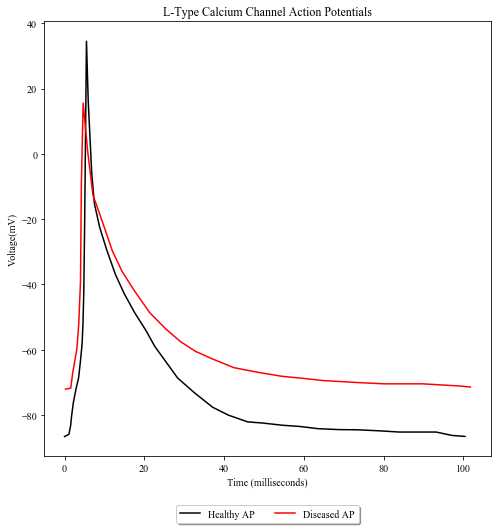
\includegraphics[scale=0.5]{ap.png}
	\caption{L-Type Calcium Channel Action Potentials}Healthy (black) and Diseased (red) action potentials used to stimulate the LTCC, based on the model by Morotto et al (2014).
\end{figure}

In an effort to \textit{upgrade} the original Calcium Release Unit mode, we aimed to model a \textit{triggered} $Ca^{2+}$ spark, or the process known as Calcium-Induced Calcium Release. In order to do this, we included a model of the Voltage-Dependent Calcium Channel, known as the L-Type Calcium Channel (LTCC). We adapted the model of LTCCs by Greenstein and Winslow \cite{Greenstein2002} to our system. We used two different action potentials to stimulatie our LTCC 1) "healthy" or WT and 2) "diseased" or Calmodulin-Dependent Kinase II over-expression (CaMKII-OE) action potentials as modeleded by Morotti et al. \cite{Morotti2014} (see figure 4.2). The LTCC model has both voltage-dependednt modes and Calcium-dependednt modes. With this model, we were able to model the rates of LTCC state transitions as a function of membrane Calcium reactions, voltage and time, according to the relationships described by Greenstein and Winslow (see Figure 4.1c), described below.

The forward rate transitions of the Voltage-dependent modes, $\alpha$ are a function of the membrane voltage, according to equation 4.17. 
\begin{equation}
\alpha = 2.0 e ^ { 0.012 \left( \mathrm { V } _ { \mathrm { m } } - 35 \right) }
\end{equation}

The reverse rate transitions of the Voltage-dependent modes, $\alpha$ are a function of the membrane voltage, according to equation 4.18. 
\begin{equation}
\beta = 0.0882 e ^ { - 0.05 \left( \mathrm { V } _ { \mathrm { m } } - 35 \right) }
\end{equation}

The forward rate transitions of the Calcium-dependent modes, $\alpha ^ { \prime }$ are a scalar multiple of $\alpha$ given by equation 4.19. 
\begin{equation}
\alpha ^ { \prime } = a \alpha
\end{equation}

The reverse rate transitions of the Calcium-dependent modes, $\beta ^ { \prime }$ are a scalar multiple of $\beta$ given by equation 4.20. 
\begin{equation}
\beta ^ { \prime } = b \beta
\end{equation}

The parameters defining the forward rate, $k_{ fy }$, and reverse rates, $k_{ ry }$, of the voltage dependent inactivation are defined by equations 4.21 through 4.24.

\begin{equation}
y _ { \infty } = 0.4 / \left( 1 + e ^ { \left( \mathrm { V } _ { \mathrm { m } } + 12.5 \right) / 5 } \right) + 0.6
\end{equation}

\begin{equation}
\tau _ { \mathrm { y } } = 340 / \left( 1 + e ^ { \left( \mathrm { V } _ { \mathrm { m } } + 30 \right) / 12 } \right) + 60
\end{equation}

\begin{equation}
k _ { \mathrm { f } , \mathrm { y } } = y _ { \infty } / \tau _ { \mathrm { y } }
\end{equation}

\begin{equation}
k _ { \mathrm { b } , \mathrm { y } } = \left( 1 - y _ { \infty } \right) / \tau _ { \mathrm { y } }
\end{equation}


In order to calculate the inward flux of Calcium through the LTCC k$_{IVin}$ and the outward flux k$_{IVout}$, we  converted the permeability of Ca$^{2+}$ P$_{Ca}$ to ions/sec using equation 4.25 and 4.26. We assume 2mM extracellular Calcium concentration. We use the following two equations where,$N_{A}$ is Avogadro's number, \textit{z} is charge,  V$_{m}$ is the membrane voltage and \textit{F} is Faraday's constant, R is the universal gas constant, and T is temperature. 


\begin{equation}
 k_{IVin} =\frac {[Ca^{2+}] \frac{N_{A}}{z} P_{Ca}4V_{m}F0.341}{RTe^{\frac {2V_{m}F}{RT}-1}}
\end{equation}


\begin{equation}
 k_{IVout} =\frac {\frac{N_{A}}{z} P_{Ca}4V_{m}Fe^{\frac {2V_{m}F}{RT}}}{RTe^{\frac {2V_{m}F}{RT}-1}}
\end{equation}





\subsection{Sarcoplasmic Reticulum Fluxes}
\subsubsection{Sarco/Endoplasmic Reticulum Calcium-ATPase (SERCA) pump kinetics}

\setcounter{figure}{2}
\begin{figure}
\centering
	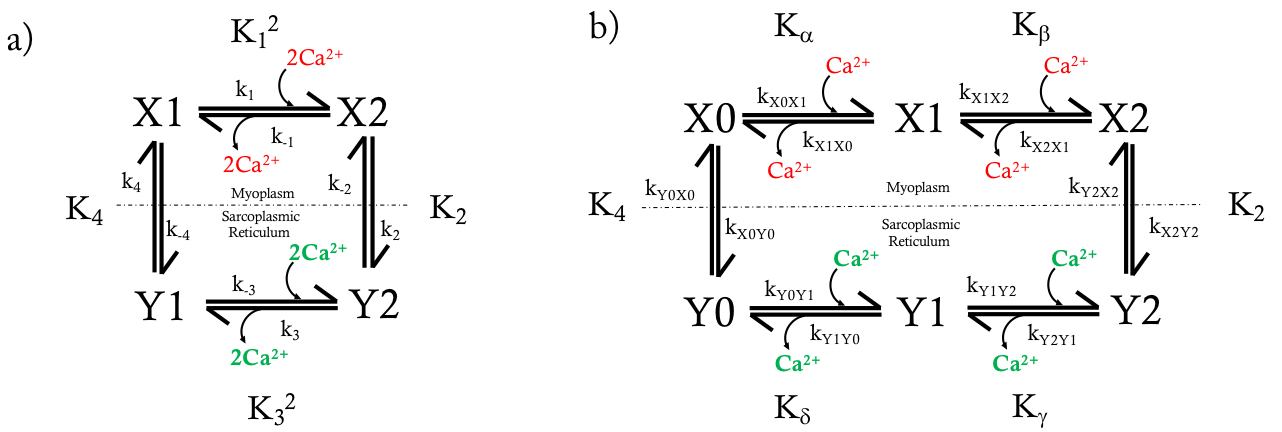
\includegraphics[scale=0.73]{SERCA2_fig.png}
	\caption{SERCA Models}
	\subcaption{Sarco/Endoplasmic Reticulum Calcium-ATPase (SERCA) Model by Higgins et al. Two cytoplasmic-facing states (X) and two sarcoplasmic reticulum-facing states (Y) translocate cytosolic Calcium (red) to the sarcoplasmic reticulum (green).}
	\subcaption{Sarco/Endoplasmic Reticulum Model. Adapted from the model by Higgins et al 2006 by separating the event of two $Ca^{2+}$ binding/unbinding into individual $Ca^{2+}$ binding/unbinding reactions. Three cytoplasmic-facing states (X) and three sarcoplasmic reticulum-facing states (Y) translocate cytosolic Calcium (red) to the sarcoplasmic reticulum (green). Reaction rates can be found in Table 4.5 }
\label{fig:SERCAHiggins} 
\end{figure}


 Of utmost importance in the dynamics of $Ca^{2+}$ during the phenomenon of CICR is the action of the SERCA pump, which is estimated to be responsible for the clearing of 70-90\% of cardiomyocyte $Ca^{2+}$ after a release event event \cite{Bers2002}. In a single forward cycle of the SERCA pump, one molecule of ATP is consumed to translocate two ions of $Ca^{2+}$ from the cytoplasm into the SR, the intracellular $Ca^{2+}$ store.  In order to explicitly model the dynamics of $Ca^{2+}$ in the myoplasm and inside the SR, it is necessary to use models that treat calcium as individual species. In order to achieve this, we adapted a model of SERCA by Higgins et al. \cite{Higgins2006} as modeled in our previous work \cite{Bartol2015} to reproduce the dynamics of SERCA2a, maintaining 140nM cytoplasmic $Ca^{2+}$ while satisfying microscopic reversibility. 

The four-state model by Higgins et al. \cite{Higgins2006} (Figure 4.3) groups both $Ca^{2+}$ binding and unbinding events into a single step (see Figure 4.3 (a) $K_{1}$ and $K_{3}$, respectively). In our adapted version of the Higgins model, we model SERCA as a six-state pump that binds (see Figure 4.3 (b) $K_{\alpha}$ and $K_{B}$) and unbinds (see Figure 4.3 (b) $K_{\gamma}$ and $K_{\delta}$) $Ca^{2+}$ ions discretely. In order to accomplish this, the equilibrium constants for binding and unbinding $Ca^{2+}$  ($K_{1}$ and $K_{3}$, respectively) needed to be split up into two rate constants for the individual binding ($K_{\alpha}$ and $K_{\beta}$) and unbinding ($K_{\gamma}$ and $K_{\delta}$) events. This was accomplished using the theory of ligand occupancy developed by Sine and Taylor \cite{Sine1979,Sine1980,Sine1981}. 

Firstly, we assume that the $Ca^{2+}$  equilibrium constant for the binding of 2 $Ca^{2+}$ ions, $K_{1}^{2}$ is the product of the individual equilibrium constants, $K_{\alpha}$ and $K_{\beta}$, according to equations 4.27-4.30, below. 
\begin{equation}
K_{1}^{2}= K_{\alpha} \times K_{\beta}
\end{equation}

\begin{equation}
K_{\alpha} = \frac{k_{X1X0}}{k_{X0X1}} 
\end{equation}

\begin{equation}
K_{\beta} = \frac{k_{X2X1}}{k_{X1X2}}
\end{equation}

\begin{equation}
K^{2}_{1}=  \frac{k_{X1X0}}{k_{X0X1}} \times \frac{k_{X2X1}}{k_{X1X2}}
\end{equation}

Because there are two sites to which  $Ca^{2+}$ can bind in state X0 and only one state to which  $Ca^{2+}$ can bind to in state X1, the relationship of the $Ca^{2+}$ binding rate constants in equation 4.31 is assumed. 

\begin{equation}
k_{X0X1}=2 \times k_{X1X2} 
\end{equation}

Likewise and in the same way, there are two sites from which  $Ca^{2+}$ can unbind in state X2 and only one site to which $Ca^{2+}$ can unbind to in state X1. And so, the relationship of the $Ca^{2+}$ unbinding rate constants in equation 4.32 is assumed. 

\begin{equation}
k_{X2X1}=2 \times k_{X1X0} 
\end{equation} 

Substituting into equation 4.30 for the rate constant relationships 4.31 and 4.32, yields equation 4.32.

\begin{equation}
K^{2}_{1}=  \frac{k_{X1X0}}{2 \times k_{X1X2}} \times \frac{2 \times k_{X1X0}}{k_{X1X2}} = \left(\frac{k_{X1X0}}{k_{X1X2}}\right)^{2}
\end{equation}

According to the relationship of the equilibrium constants in equations 4.31-32, the relationship between the equilibrium constants $K_{\alpha}$ and $K_{\beta}$ is the one given by equation 4.34.

\begin{equation}
K_{\alpha}= \frac{K_{\beta}}{4}
\end{equation}

We solve for the individual rate constants by substitute the relationship given in 4.34 into equation 4.35 yielding equations 4.36-38. 


\begin{equation}
K_{1}= \sqrt{K_{\alpha} \times K_{\beta}}
\end{equation}


\begin{equation}
K_{1}= \sqrt{ \frac{K_{\beta}^2}{4}}
\end{equation}

\begin{equation}
K_{\alpha}= \frac{K_{1}}{2} 
\end{equation}

\begin{equation}
K_{\beta}= K_{1} \times 2
\end{equation}



In the same way, we can derive the individual rate constants, $K_{\gamma}$ and $K_{\delta}$ from the equilibrium constant for the unbinding of 2 $Ca^{2+}$ ions, $K_{3}^{2}$.  

\begin{equation}
K_{3}^{2}= K_{\gamma} \times K_{\delta}
\end{equation}

\begin{equation}
K_{\gamma} = \frac{k_{Y1Y2}}{k_{Y2Y1}} 
\end{equation}

\begin{equation}
K_{\delta} = \frac{k_{Y0Y1}}{k_{Y1Y0}}
\end{equation}

\begin{equation}
K^{2}_{3}=   \frac{k_{Y1Y2}}{k_{Y2Y1}} \times \frac{k_{Y0Y1}}{k_{Y1Y0}}
\end{equation}

Because there are two sites to which  $Ca^{2+}$ can unbind from in state Y2 and only one state from which $Ca^{2+}$ can unbind state X1, the relationship $Ca^{2+}$ unbinding rate constants in equation 4.43 is assumed. 

\begin{equation}
k_{Y1Y0}=2 \times k_{Y2Y1} 
\end{equation}

In the same way, there are two sites to which $Ca^{2+}$ can bind in state Y0 and only one site to which $Ca^{2+}$ can bind to in state Y1. As such, the relationship of the $Ca^{2+}$ binding rate constants in equation 4.44 is assumed. 


\begin{equation}
k_{Y0Y1}=2 \times k_{Y1Y2} 
\end{equation} 

Substituting into equation 4.42 for the rate constant relationships 4.43 and 4.44, yields equation 4.45.

\begin{equation}
K^{2}_{3}=  \frac{k_{Y1Y2}}{2 \times k_{Y1Y0}} \times \frac{2 \times k_{Y1Y2}}{k_{Y1Y0}} = \left(\frac{k_{Y1Y2}}{k_{Y1Y0}}\right)^{2}
\end{equation}

According to the relationship of the equilibrium constants in equations 4.43 and 4.44, the relationship between the rate constants $K_{\gamma}$ and $K_{\delta}$ is the one given by equation 4.46.

\begin{equation}
K_{\delta}= \frac{K_{\gamma}}{4}
\end{equation}

We solve for the individual rate constants by substituting the relationship given in 4.46 into equation 4.47 yielding equations 4.48-4.50. 


\begin{equation}
K_{3}= \sqrt{K_{\gamma} \times K_{\delta}}
\end{equation}


\begin{equation}
K_{3}= \sqrt{\frac{K_{\gamma}^2}{4}}
\end{equation}

\begin{equation}
K_{\gamma}= K_{3} \times 2
\end{equation}

\begin{equation}
K_{\delta}= \frac{K_{3}}{2} 
\end{equation}

According to Higgins et al., the relationship between the Gibbs Free energy of 1 molecule of ATP and the kinetic cycle is given by equation 4.51.
\begin{equation}
K _ { 1 } ^ { 2 }   K _ { 2 } K _ { 3 } ^ { 2 } K _ { 4 } = e ^ { \Delta \mathrm { G } _ { \mathrm { ATP } } ^ { 0 } / \mathrm { RT } }
\end{equation}

Using the rate constants described in Table 4.5 and the relationships described above, yields a Gibbs free energy of -47.0943 kJ/mol. The product of the forward rates constants equals the product of the reverse rate constants. At steady state, this is also true for the product of the forward reaction rates and the product of the reverse reaction rates, satisfying detailed balance. Lastly, the pump reaches steady state at a cytosolic concentration, $Ca^{2+}_{ \mathrm { cyt } _ { \mathrm { ss } } }$, of 140nM and a SR concentration, $Ca^{2+} _ { \mathrm { sr } _ { \mathrm { ss } } } $, of 1.3mM.

\begin{equation}
Ca^{2+} _ { \mathrm { sr } _ { \mathrm { ss } } } = \frac {Ca^{2+}_{ \mathrm { cyt } _ { \mathrm { ss } } } } { K _ { 1 } K _ { 3 } \sqrt { K _ { 2 } K _ { 4 } } }
\end{equation}

\setcounter{figure}{3}

\begin{figure}
\centering
	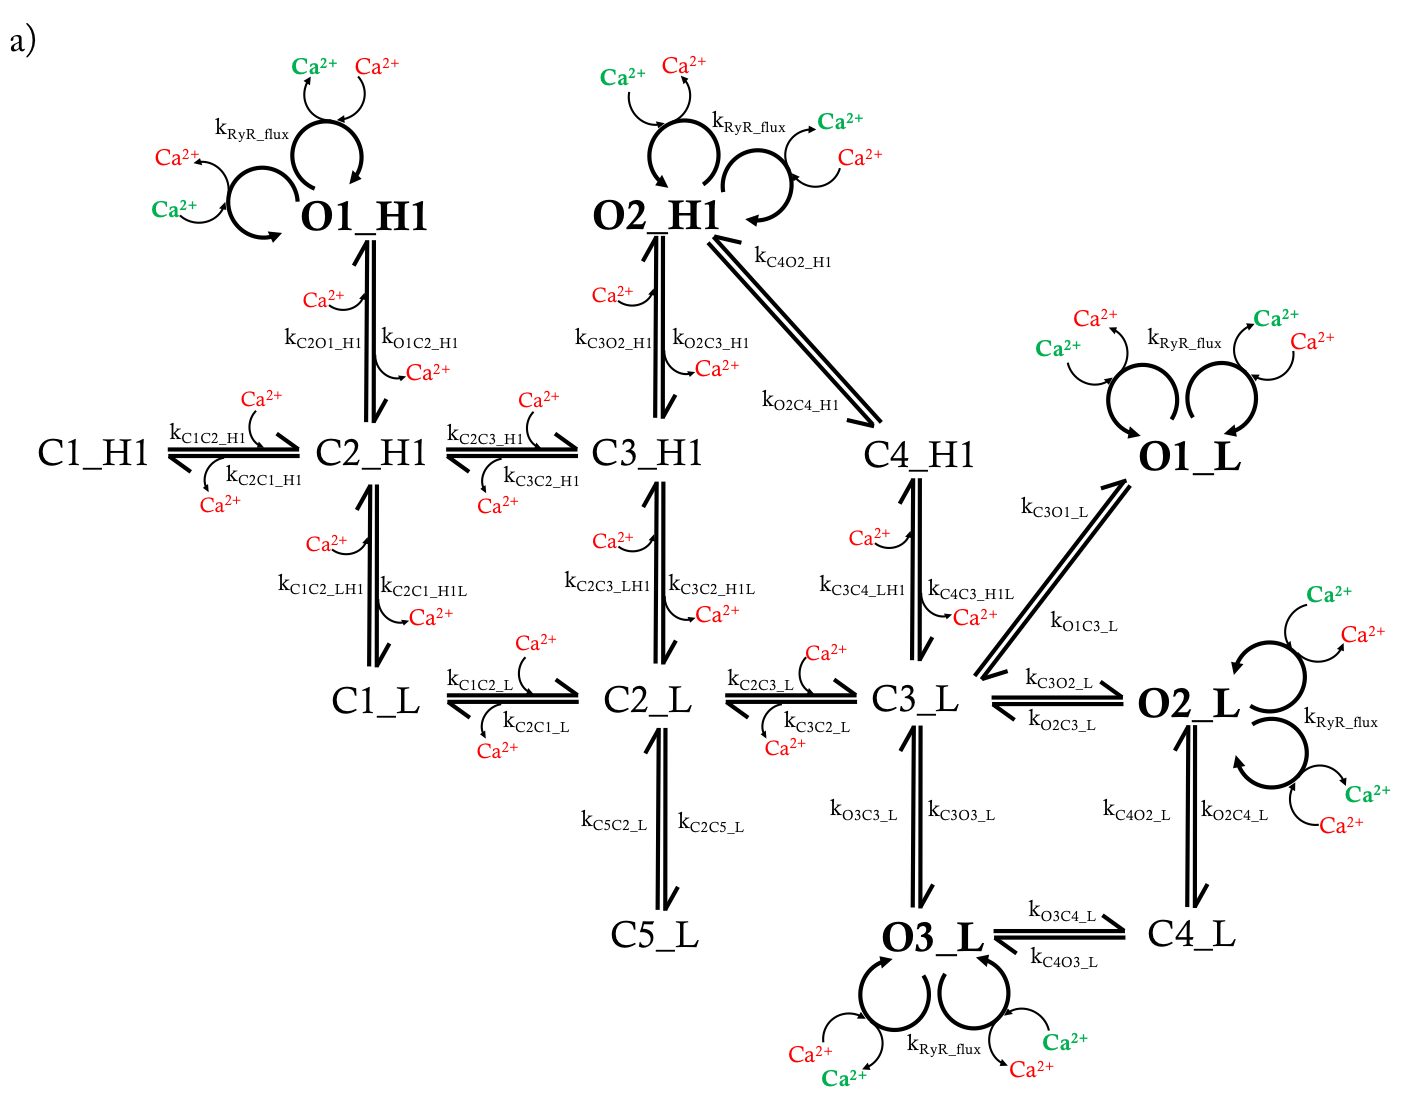
\includegraphics[scale=0.65]{RyRflux_fig.png}	
	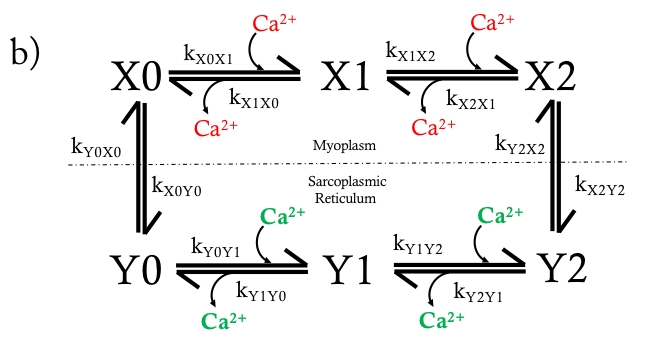
\includegraphics[scale=0.6]{SERCAflux_fig.png}
	\caption{Sarcoplasmic Reticulum Fluxes}
	\subcaption{Ryanodine Receptor Markov Model. Adapted from the Markov Model by Saftenku et al. (2001); Nine closed (C) states and five open (O) states describe the kinetic scheme of the Ryanodine Receptor. Cytosolic Calcium (Red) binds to closed states in High (H1) and Low (L) gating modes. In open states, Sarcoplasmic Reticulum Calcium (Green) and Cytosolic Calcium are translocated through the receptors. Reaction rates can be found in Table 4.4.}
	\subcaption{Sarco/Endoplasmic Reticulum Model. Adapted from the model by Higgins et al 2006. Three cytoplasmic-facing states (X) and three sarcoplasmic reticulum-facing states (Y) translocate cytosolic Calcium (red) to Calcium the sarcoplasmic reticulum (green). Reaction rates can be found in Table 4.5}
\label{fig:SRfluxes} 
\end{figure}

\subsubsection{Ryanodine Receptor (RyR) kinetics}

In order to simulate a triggered Ca$^{2+}$ spark, it was necessary to model the complexities of the Sarcoplasmic Reticulum Ca$^{2+}$ release channel, the Ryanodine Receptor. Hake's original simulations used a simplistic, binary model of RyR that could exist in either an open or a closed state. Once a certain voltage was sensed, the RyR would close and never re-open. Most notably the RyR in these simulations did not activate in response to alterations in Ca$^{2+}$ levels, but instead were set to "open" to initiate the spark. RyR is known to interact with 30+ binding partners \cite{Song2011}, and thus, can exist in a multitude of states. In an attempt model this complexity, we incorporated a Markov model of RyR that captures its low and high gating modes as well as its ability to bind Ca$^{2+}$ as a basis for its activation.

We adapted the Markov model of RyR dynamics by Saftenku et al. \cite{Saftenku2001} for use in MCell simulations (see Figure 4.4a). Coincidentally, this was the same model of RyR used by Koh et al in their MCell simulations using simplistic geometries\cite{Koh2006}. 

The parameters for the RyR model (see Table 4.4) were used with little adaptation with the exception of the RyR flux rate. For the purpose of our simulations, the RyR flux rate had to be converted to units of Ca$^{2+}$ ions/second. This was accomplished using the single-channel current, measured at 0.35 pA at 1mM by Guo et al \cite{Guo2012} and the relationship described in equation 4.42, below.

\begin{equation}
k_{RyRflux} = \frac {I^{RyR}6.242\times 10^{18}\frac{Charge}{Coulomb}}{\left[ Ca^{2+}\right] z} = \frac{9.01\times10^{-9}  Ca^{2+}ions}{s}
\end{equation}

Amps are defined as units of $\frac{Coulomb}{second}$. Thus, the RyR current, $I^{RyR}$ in pA can be converted to charges by multiplying the conversion factor, $6.242\times 10^{18}\frac{Charge}{Coulomb}$. Using the 1mM concentration of Calcium and a charge or, \textit{z}, value of 2, equals to a rate of $ 9.01\times10^{-9}\frac{ Ca^{2+}ions}{s}$.
%Reversal potential -2.4mV and Voltage of ER = 0mV





\begin{comment}

\begin{equation}
\lambda=\sqrt {4D\Delta t}
\label{eq:dimensionless radial distance}
\end{equation}

\begin{equation}
\tilde{r}={\frac{r}{\lambda}}
\label{eq:dimensionless radial distance}
\end{equation}

\begin{equation}
\overline {l}_{\bot}=\sqrt {\frac {4D\Delta t}{\pi }}
\label{eq:Orthogonal step length}
\end{equation}


\begin{equation}
\overline {l}_{r}=\overline {l}_{\bot}\times 2
\label{eq:radial diffusional step length}
\end{equation}


\begin{equation}
{N}_{H}={N}_{\si{\angstrom}}\overline {l}_{\bot}{A}_{ET}{[A]}_{o}
\label{eq:Orthogonal step length}
\end{equation}



Where ${[A]}_{o}$ is the initial concentration of the species, ${A}_{ET}$ is the area of the effector tile, $\overline {l}_{\bot}$ is the average orthogonal step length, ${N}_{\si{\angstrom}}$ is Avogadro's number and ${N}_{H}$ is the number of hits.




\begin{equation}
[ \mathrm { ATP } ] _ { \mathrm { tot } } = [ \mathrm { ATP } ] _ { \mathrm { tot } - \mathrm { i } } = [ \mathrm { ATP } ] _ { \mathrm { tot } - \mathrm { ss } }
\end{equation}

\begin{equation}
[ \mathrm { ATP } ] _ { \mathrm { ss } } = [ \mathrm { ATP } ] _ { \mathrm { tot } } - [ \mathrm { CaATP } ] _ { \mathrm { ss } } - [ \mathrm { MgATP } ] _ { \mathrm { ss } }
\end{equation}

\begin{equation}
\left[ ATP\right]_{ss} = \frac{k^{MgATP}_{r}\left[ MgATP\right] _{ss}+J^{MgATP}_{xfer}\dfrac {V_{myo}}{V_{ss}}}{k^{MgATP}_{f}\left[ Mg\right] _{SS}}
\end{equation}


\begin{equation}
\begin{aligned} \frac { \mathrm { d } [ \mathrm { CaATP } ] _ { \mathrm { ss } } } { \mathrm { d } t } = & - J _ { \mathrm { xfer } } ^ { \mathrm { CaATP } } \frac { V _ { \mathrm { myo } } } { V _ { \mathrm { ss } } } + k _ {f} ^ { \mathrm { CaATP } } [ \mathrm { Ca } ] _ { \mathrm { ss } } [ \mathrm { ATP } ] _ { \mathrm {ss} } -k _ {r} ^ { \mathrm { CaATP } } [ \mathrm { CaATP } ] _ { \mathrm { ss } } \end{aligned}
\end{equation}


\begin{equation}
\frac{d\left[CaATP\right]_{ss}}{dt} = 0
\end{equation}

\begin{equation}
\left[ CaATP\right] _{ss}=-\frac {J^{CaATP}_{xfer}\dfrac {V_{myo}}{V_{ss}}+k^{CaATP}_{f}\left[ Ca\right] _{ss}\left[ ATP\right] _{ss}}{k^{CaATP}_{r}}
\end{equation}


\begin{equation}
\begin{aligned} \frac { \mathrm { d } [ \mathrm { MgATP } ] _ { \mathrm { ss } } } { \mathrm { d } t } = & - J _ { \mathrm { xfer } } ^ { \mathrm {MgATP } } \frac { V _ { \mathrm { myo } } } { V _ { \mathrm { ss } } } + k _ {f} ^ { \mathrm { MgATP } } [ \mathrm { Mg } ] _ { \mathrm { ss } } [ \mathrm { ATP } ] _ { \mathrm {ss} } -k _ {r} ^ { \mathrm {MgATP } } [ \mathrm { MgATP } ] _ { \mathrm { ss } } \end{aligned}
\end{equation}


\begin{equation}
\frac{d\left[MgATP\right]_{ss}}{dt} = 0
\end{equation}

\begin{equation}
\left[ MgATP\right] _{ss}=-\frac {J^{MgATP}_{xfer}\dfrac {V_{myo}}{V_{ss}}+k^{MgATP}_{f}\left[ Mg\right] _{ss}\left[ ATP\right] _{ss}}{k^{MgATP}_{r}}
\end{equation}

\end{comment}


 \section{Results and Discussion}

\subsection{Buffer and Fluorophore Dynamics}
We began our investigations by building the model from a baseline, using cytosolic buffers, sarcolemmal pumps, and fluorophores as the subjects of our simulations. To make sure equilibrium is maintained in our simulations, we investigated the dynamics of Calcium and its buffers in simulations lacking the sarcollemal stimulus, L-Type Calcium Channel. Because Ryanodine receptors are known to spontaneously activate in the presence of Calcium\cite{Cheng1993,Cannell1995}, and SERCA itself is known to act as a buffer\cite{Higgins2006} we eliminated these effects to establish that the baseline system maintains equilibrium. A question addressed by Hake et al. in their original investigation centered on the effect of fluorophores in the simulations. We also decided to test this effect in our initial simulations. 

The system dynamics comparing the effects of the fluorophores on the baseline system (containing only buffers and sarcollemal pumps) are nearly identical (see Figure 4.5). The most pronounced effect is on the cytosolic buffer, Troponin C (See Figure 4.5e) which differs, on average, only 14 molecules between simulations with and without fluorophores. Due to a high concentration of TRPN and TRPN-Ca$^{2+}$ in the simulations (70 $\mu$M total, 13.2 $\mu$M bound to Calcium, 56.8 $\mu$M free), this corresponds to a difference of 0.036\% on average between the two systems, which is arguably negligible. 

\setcounter{figure}{4}
\begin{figure}
\centering
	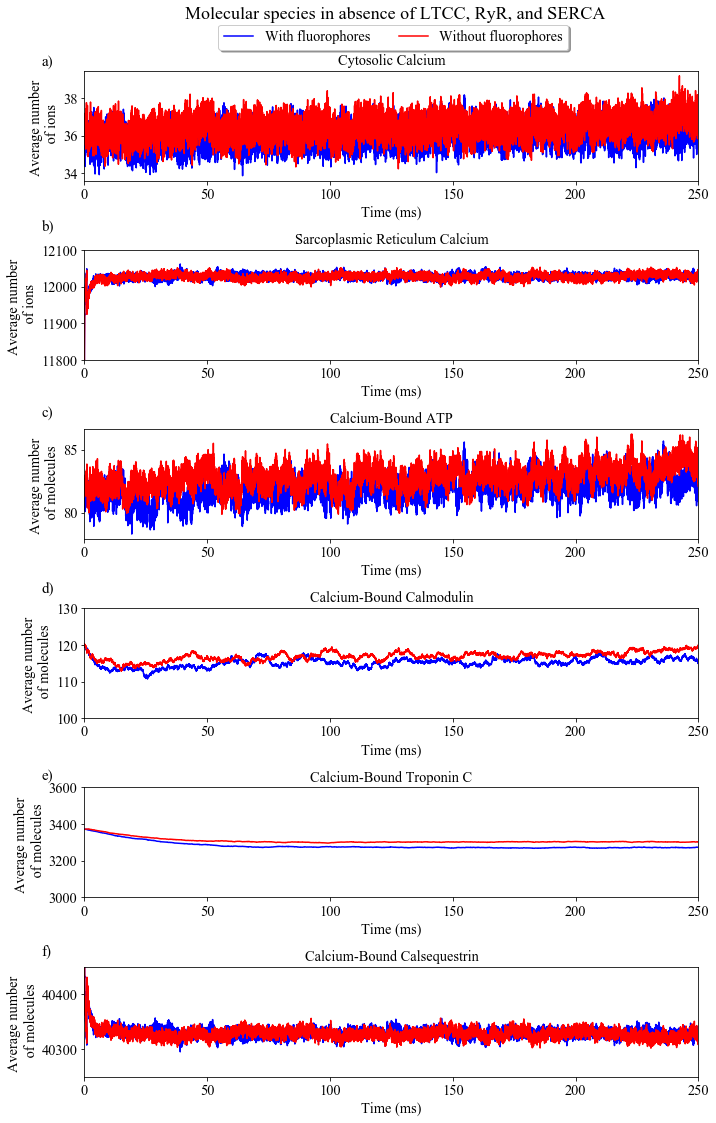
\includegraphics[scale=0.45]{buffer_fluo_molecules_c_Comparison.png}
	\caption{Molecular species in absence of LTCC, RyR and SERCA} Comparing simulations with only RyR (blue) and RyR and SERCA(red)
	\subcaption{Cytosolic Calcium dynamics; \textbf{(b)} Sarcoplasmic Reticulum Calcium dynamics; \textbf{(c)} Calcium-bound ATP; \textbf{(d)} Calcium-bound Calmodulin; \textbf{(e)} Calcium-bound Troponin-C; \textbf{(f)}Calcium-bound Calsequestrin}
\label{fig:buffer_fluo} 
\end{figure}

\subsection{Ryanodine Receptor activation absence of LTCC in response to single action potential  LTCC alterations}

In order to validate our model, we sought confirmation that that our system could generate spontaneous Ca$^{2+}$ sparks without an LTCC stimulus as observed in experiments \cite{Cheng1993,Lopez-Lopez1994,Cannell1995}. In order to test this, we simulated our CRU system in absence of an action potential stimulus but in the presence of RyR with and without SERCA (see Figure 4.6). Though the average of total number of RyR openings (n=128) are low, there is a non-zero probability that RyR in be triggered spontaneously.

\setcounter{figure}{5}
\begin{figure}
\centering
	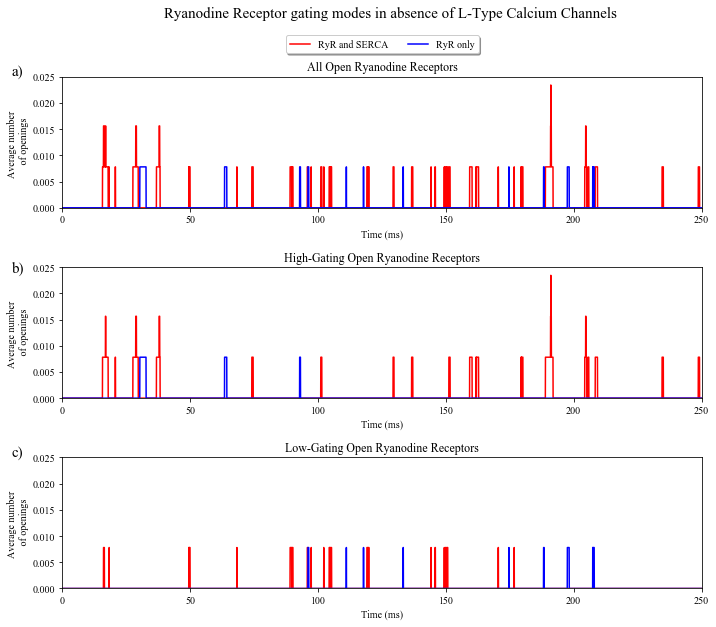
\includegraphics[scale=0.6]{buffer_fluo_RyR_r_Comparison.png}
	\caption{Ryanodine Receptor gating modes in absence of L-Type Calcium Channels} RyR and SERCA (red) and only RyR (blue)
	\subcaption{All open Ryanodine Receptors; \textbf{(b)} High-gating open Ryanodine Receptors; \textbf{(c)} Low-gating open Ryanodine Receptors}
\label{fig:Buffer RyR} 
\end{figure}

Having established that RyR are capable of firing spontaneously in the absence of an AP stimulus, we sought to confirm that a single LTCC could activate RyRs as previously demonstrated by Sobie et al\cite{Sobie2002}. Figure 4.7 demonstrates that one LTCC with a single action potential is sufficient to activate RyR. 

\setcounter{figure}{6}
\begin{figure}
%\centering
	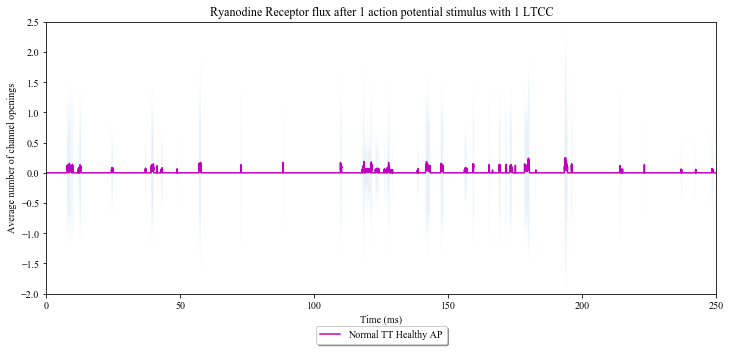
\includegraphics[scale=0.61]{RyRflux_1AP_1LTCC.png}
	\caption{Ryanodine Receptor flux after 1 action potential stimulus with 1 LTCC} Average number of openings of RyR in normal T-Tubules simulated with a single L-Type Calcium Channel and the healthy action potential (purple). Standard deviations are shown in light blue.
\label{fig:RyR flux 1 LTCC} 
\end{figure}

Following our simulations with 1 LTCC, we sought to understand the effect that increasing the number of LTCC would have on triggered Calcium release. We comparatively investigated CICR with 1, 2, 4, 6, 8, and 10 LTCC. We predicted that increasing LTCC would result in increased gain, or SR Ca$^{2+}$ efflux through RyR. Consistent with experimental findings, \cite{Cannell1995} increasing the LTCC results in positive gain as demonstrated in Figure 4.8.

\setcounter{figure}{7}
\begin{figure}
\centering
	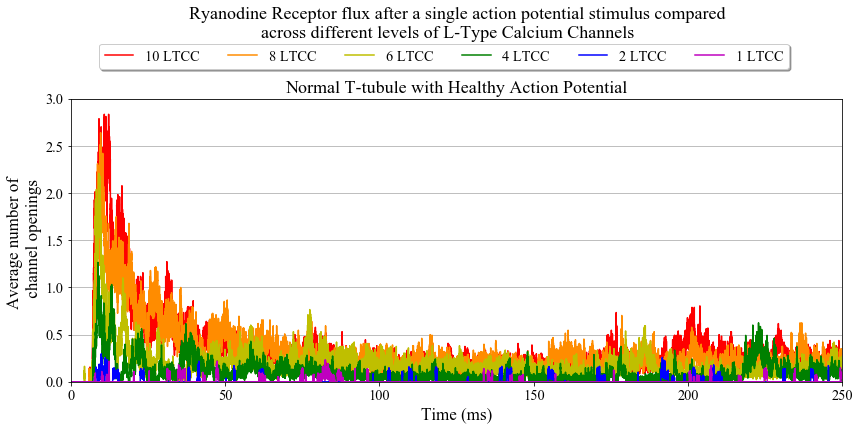
\includegraphics[scale=0.52]{RyRflux_1AP_LTCC_hn_Comparison.png}
	\caption{Ryanodine Receptor flux after 1 action potential stimulus compared across L-Type Calcium Channels} Average number of openings of RyR in normal T-Tubules with a healthy action potential compared across a series of LTCC numbers: 10 LTCC (red), 8 LTCC (orange), 6 LTCC (yellow), 4 LTCC (green), 2 LTCC (blue), 1 LTCC (purple)
\label{fig:hnhd 1 AP LTCC RyR } 
\end{figure}

\subsection{Activation in response to single action potential}
With the use of the LTCC model developed by Greenstein and Winslow \cite{Greenstein2002}, we were able to interrogate the effect of diseases sarcolemmal stimuli on Ca$^{2+}$ signaling (see Figure 1). A number of recent studies have examined disease electrical stimulus phenotypes \cite{Morotti2014, Edwards2014}, demonstrating that indeed, left-ventricle mouse action potentials have pronounced effects. We chose to model the effect of Calcium-Calmodulin Kinase II over-expression (CaMKII-OE) which results heart-failure in mice.

The effect of the diseased action potential on Calcium signaling is the same across all L-Type Calcium channels levels. The diseased AP leads to an overall increase in calcium levels in the cytosol (see figure 4.9) as a result of frequent activations of Ryanodine Receptors (see figure 4.10). This is an expected result, as depolarization of the membrane is relatively higher in the later half of the AP in the CAMKII-OE disease state. Most interesting is the later-stage RyR activation seen in the disease states. Significantly more RyR fire at later stages of the AP in diseased states compared to those with a healthy AP. This will undoubtedly affect the synchronous firing of the calcium release units, a phenomenon known as Late Ca$^{2+}$ Sparks (LCS) that have recently been observed in models of CAMKII-OE \cite{Fowler2017}. It should be noted that his effect is seen in all variations of LTCC numbers but only the cases of 1 LTCC and 4 LTCC are shown here in the interest of brevity. 

Our result is consistent with the Ca$^{2+}$ signaling profile  CAMKII-OE models in mouse models, which indicate more frequent sparks as well as greater time to peak calcium and larger maximal rate of rise \cite{Guo2012a}. This effect that is most apparent in figure 4.9, where levels of Ca$^{2+}$  release are higher overall, across all cases of LTCC alterations and have longer rise times. 


\setcounter{figure}{8}
\begin{figure}
\centering
	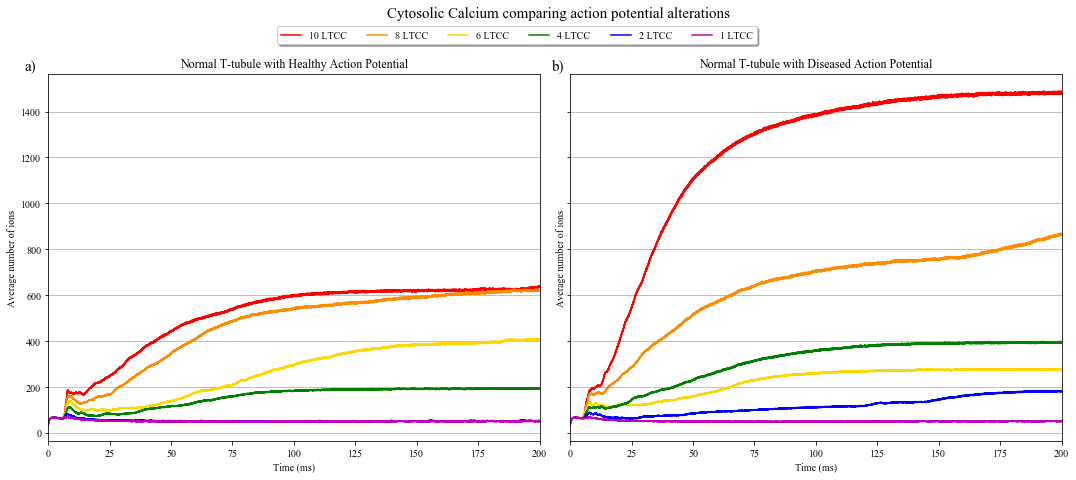
\includegraphics[scale=0.42]{cytCa_hnhd_Comparison.png}
	\caption{Cytosolic Calcium comparing action potential alterations}
	\subcaption{Cytosolic calcium in Normal T-Tubules with healthy action potential across range of L-Type Calcium Channels; \textbf{(b)} Cytosolic calcium in Normal T-Tubules with diseased action potential across range of L-Type Calcium Channels;}
	\label{fig:hnhd Calcium}
\end{figure}




\setcounter{figure}{9}
\begin{figure}
\centering
	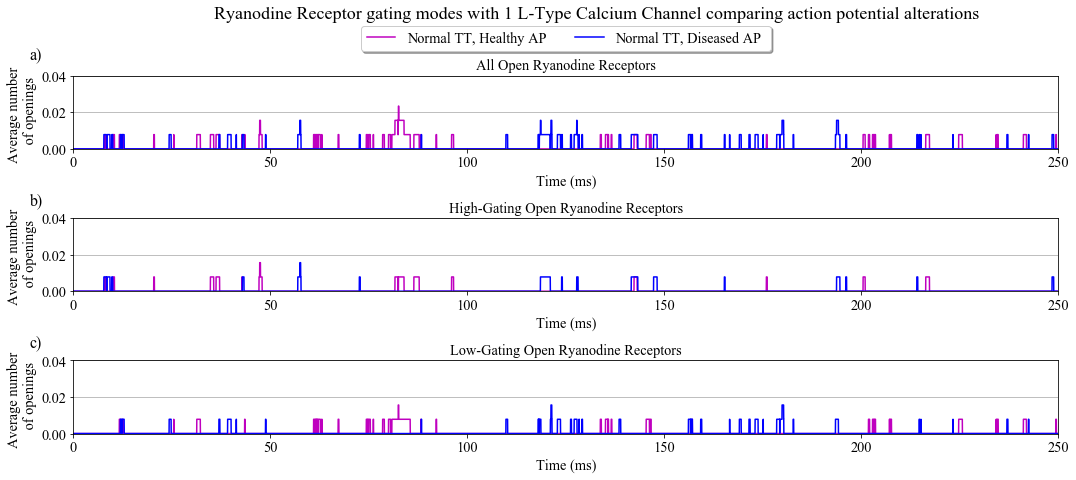
\includegraphics[scale=0.4]{hnhd1RyR_r_1AP_Comparison.png}
	\caption{Ryanodine Receptor gating modes with 1 L-Type Calcium Channel comparing action potential alterations}Healthy action potential (purple), Diseased action potential (blue)
	\subcaption{All open Ryanodine Receptors; \textbf{(b)} High-gating open Ryanodine Receptors; \textbf{(c)} Low-gating open Ryanodine Receptors}
\label{fig:hnhd 1 LTCC 1 AP RyR} 
\end{figure}

\setcounter{figure}{10}
\begin{figure}
\centering
	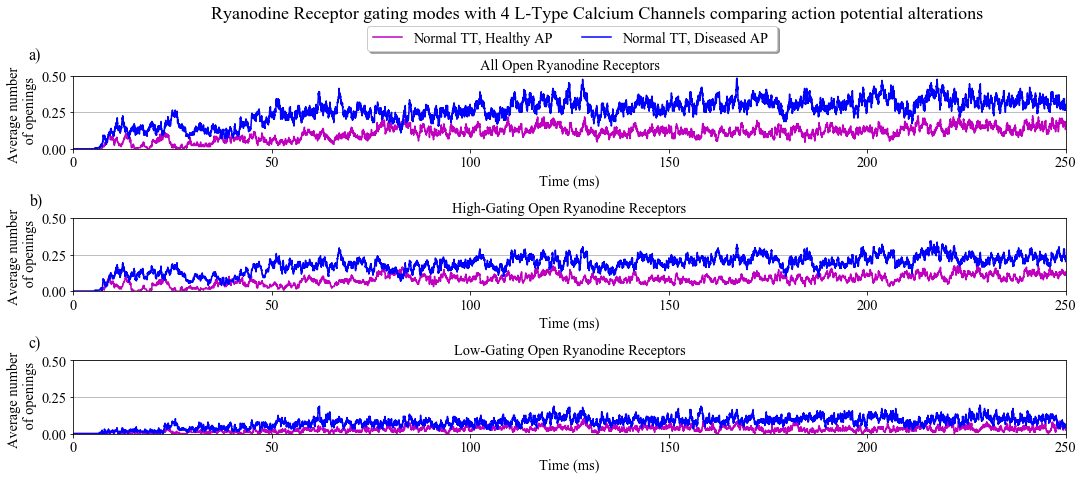
\includegraphics[scale=0.4]{hnhd4RyR_r_Comparison.png}	\caption{Ryanodine Receptor gating modes with 4 L-Type Calcium Channels comparing action potential alterations}Healthy action potential (purple), Diseased action potential (blue)
	\subcaption{All open Ryanodine Receptors; \textbf{(b)} High-gating open Ryanodine Receptors; \textbf{(c)} Low-gating open Ryanodine Receptors}
\label{fig:hnhd 4 LTCC 1 AP RyR} 
\end{figure}

In an additional effort to understand disease phenotypes in heart failure, we investigated the effects of T-Tubule deformations on cardiac calcium release units. In the literature, is effect is termed "de-tubulation" of myocyte tissue. Because of the close juxtaposition of T-Tubule membranes and SR membranes, we predicted an increase in the dyadic space would result in less RyR activation and overall lower cytosolic calcium. 

\subsection{Activation in response to multiple action potentials}



\setcounter{figure}{11}
\begin{figure}
\centering
	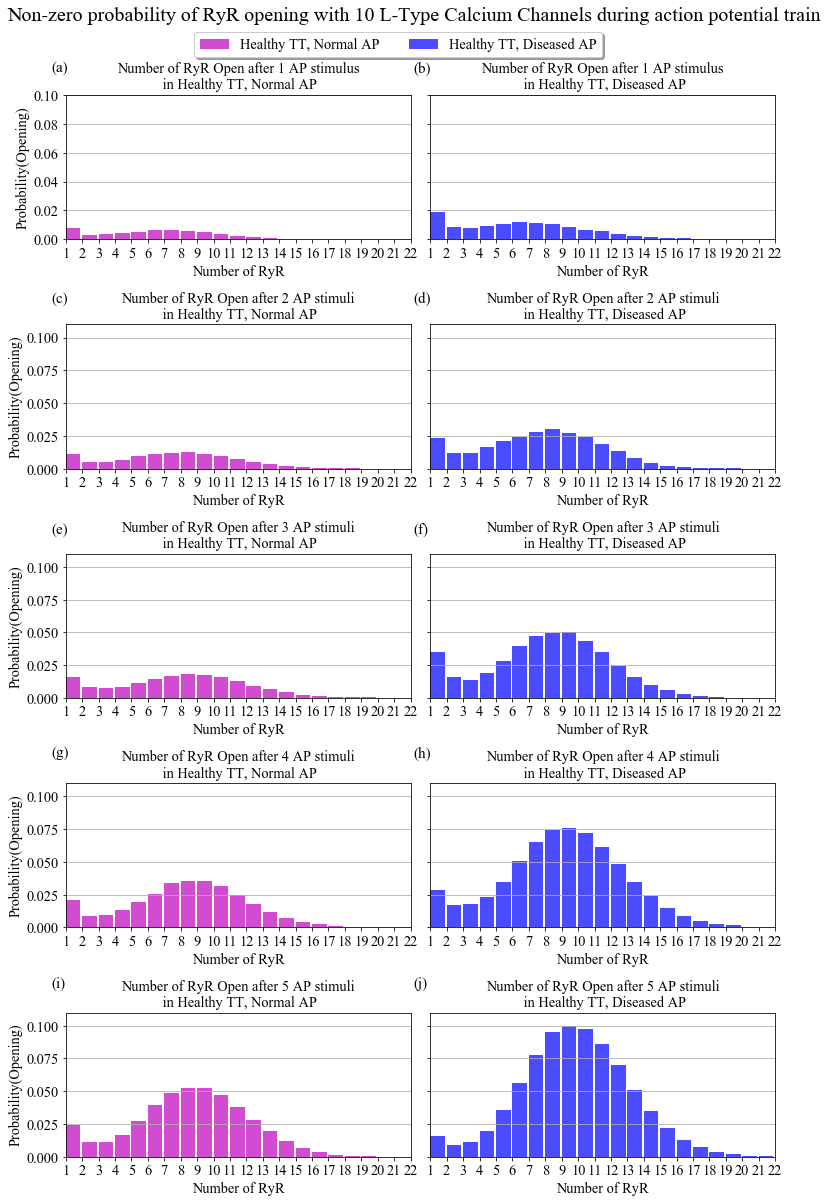
\includegraphics[scale=0.45]{probabilities_RyRopen_hnhd_1-5_AP_Comparison.png}
		\caption{}
	\subcaption{Number of RyR open after 1 normal action potential stimulus in healthy t-tubules; \textbf{(b)} Number of RyR open after 1 diseased action potential stimulus in healthy t-tubules; \textbf{(c)} Number of RyR open after 2 normal action potential stimuli in healthy t-tubules; \textbf{(d)} Number of RyR open after 2 diseased  action potential stimuli in healthy t-tubules; \textbf{(e)} Number of RyR open after 3 normal action potential stimuli in healthy t-tubules; \textbf{(f)}Number of RyR open after 3 diseased action potential stimuli in healthy t-tubules; \textbf{(g)} Number of RyR open after 4 normal action potential stimuli in healthy t-tubules; \textbf{(g)}Number of RyR open after 4 diseased action potential stimuli in healthy t-tubules; \textbf{(i)} Number of RyR open after 5 normal action potential stimuli in healthy t-tubules; \textbf{(j)}Number of RyR open after 5 diseased action potential stimuli in healthy t-tubules;}
\label{fig:probabilities} 
\end{figure}


\setcounter{figure}{12}
\begin{figure}
\centering
	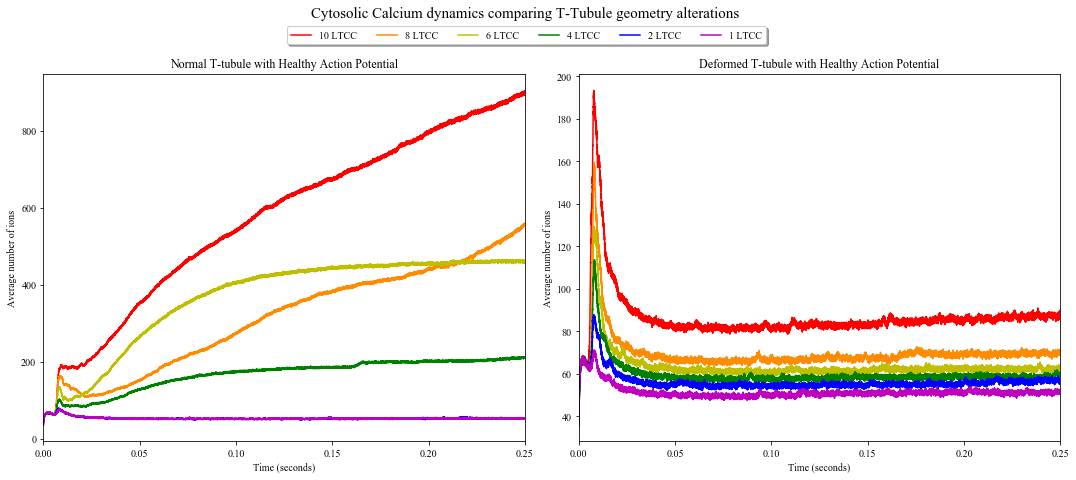
\includegraphics[scale=0.4]{cytCa_geom_Comparison.png}
		\caption{Cytosolic Calcium Calcium dynamics comparing T-Tubule geometry alterations}10 LTCC (red), 8 LTCC (orange), 6 LTCC (yellow), \\ 4 LTCC (green), 2 LTCC (blue), 1 LTCC (purple)
	\subcaption{Normal T-Tubule with Healthy action potential showing Calcium dynamics in the cytosol}
	\subcaption{Deformed T-Tubule with Healthy action potential showing Calcium dynamics in the cytosol}
\label{fig:geometry comparison} 
\end{figure}

 \section{Conclusions}



 \section{Supplementary Information}
\begin{table}[h]
\centering
\caption{Parameters of Calcium buffering species}
\resizebox{\textwidth}{!}{\begin{tabular}{ccccc}
\hline
\textbf{Parameter} & \textbf{Description} & \textbf{Value} & 
\textbf{Units} & \textbf{Reference} \\
\hline
D$^{cyt}$$_{Ca}$ & Diffusion constant of Ca$^{2+}$ (in cytosol 
and SR) & 2.2 x 10$^{6}$ & cm$^{2}$s$^{-1}$ & Hake et al. 
(2012); Louch et al. (2010) \\
\hline
D$^{cyt}$$_{ATP\_Ca}$ & Diffusion constant of Ca$^{2+}$-bound 
ATP in cytosol & 1.4 x 10$^{-6}$ & cm$^{2}$s$^{-1}$ & Hake et 
al. (2012); Valent et al (2007) \\
\hline
$[$Ca$^{2+}$$]$$_{cyt}$ & Initial Concentration of Ca$^{2+}$ 
in cytosol & 140 x 10$^{-9}$ & M & Hake et al. (2012) \\
\hline
$[$ATP$]$$_{cyt}$ & Free ATP concentration in cytosol & 454.682 x 10
$^{-6}$ & M & Hake et al. (2012); Bers (2001) \\
\hline
$[$ATP-Ca$]$$_{cyt}$ & Ca$^{2+}$-bound ATP concentration in 
cytosol & 318 x 10$^{-9}$ & M & Hake et al. (2012) \\
\hline
$^{ATP}$k$_{on}$ & ATP Ca$^{2+}$ on rate & 2.25 x 10$^{8}$ & 
M$^{-1}$s$^{-1}$ & Hake et al. (2012); Picht et al. (2011); Bers 
(2001) \\
\hline
$^{ATP}$k$_{off}$ & ATP Ca$^{2+}$ off rate & 450 x 10$^{2}$ 
& s$^{-1}$ & Hake et al. (2012); Picht et al. (2011) \\
\hline
D$^{cyt}$$_{CMDN}$ & Diffusion constant of Calmodulin in cytosol & 
25 x 10$^{-8}$ & cm$^{2}$s$^{-1}$ & Hake et al. (2012); 
Michailova et al. (2002) \\
\hline
D$^{cyt}$$_{CMDN\_Ca}$ & Diffusion constant of Ca$^{2+}$-bound 
Calmodulin in cytosol & x 10$^{-6}$ & cm$^{2}$s$^{-1}$ & Hake 
et al. (2012); \\
\hline
$[$CMDN$]$$_{cyt}$ & Free Calmodulin concentration in cytosol & 
23.529 x 10$^{-6}$ & M & Hake et al. (2012); Fabiato (1983) \\
\hline
$[$CMDN-Ca$]$$_{cyt}$ & Ca$^{2+}$-bound Calmodulin concentration 
in cytosol & 471 x 10$^{-9}$ & M & Hake et al. (2012) \\
\hline
$^{CMDN}$k$_{on}$ & Calmodulin Ca$^{2+}$ on rate & 34 x 10$^{
6}$ & M$^{-1}$s$^{-1}$ & Hake et al. (2012); Robertson et al 
(1981); Picht et al. (2011) \\
\hline
$^{CMDN}$k$_{off}$ & Calmodulin Ca$^{2+}$ off rate & 238 & s
$^{-1}$ & Hake et al. (2012); Robertson et al (1981) \\
\hline
D$^{cyt}$$_{TRPN}$ & Diffusion constant of Troponin-C in cytosol & 
0 & cm$^{2}$s$^{-1}$ & Hake et al. (2012) \\
\hline
D$^{cyt}$$_{TRPN\_Ca}$ & Diffusion constant of Ca$^{2+}$-bound 
Troponin-C in cytosol & 0 & cm$^{2}$s$^{-1}$ & Hake et al. (2012) 
\\
\hline
$[$TRPN$]$$_{cyt}$ & Free Troponin-C concentration in cytosol & 56.8 
x 10$^{-6}$ & M & Hake et al. (2012); Bondarenko et al. (2004) \\
\hline
$[$TRPN-Ca$]$$_{cyt}$ & Ca$^{2+}$-bound Troponin-C concentration 
in cytosol & 13.2 x 10$^{-6}$ & M & Hake et al. (2012) \\
\hline
$^{TRPN}$k$_{on}$ & Troponin-C Ca$^{2+}$ on rate & 32.7 x 10
$^{6}$ & M$^{-1}$s$^{-1}$ & Hake et al. (2012); Bondarenko et 
al. (2004) \\
\hline
$^{TRPN}$k$_{off}$ & Troponin-C Ca$^{2+}$ off rate & 19.6 & s
$^{-1}$ & Hake et al. (2012); Bondarenko et al. (2004) \\
\hline
D$^{cyt}$$_{Fluo4}$ & Diffusion constant of Fluo-4 in cytosol & 42 
x 10$^{-8}$ & cm$^{2}$s$^{-1}$ & Hake et al. (2012); Picht et 
al. (2011) \\
\hline
D$^{cyt}$$_{Fluo4\_Ca}$ & Diffusion constant of Ca$^{2+}$
-bound Fluo-4 in cytosol & 42 x 10$^{-8}$ & cm$^{2}$s$^{-1}$ & 
Hake et al. (2012) \\
\hline
$[$Fluo4$]$$_{cyt}$ & Free Fluo-4 concentration in cytosol & 22.186 x 
10$^{-6}$ & M & Hake et al. (2012); Picht et al. (2011) \\
\hline
$[$Fluo4-Ca$]$$_{cyt}$ & Ca$^{2+}$-bound Fluo-4 concentration in 
cytosol & 2.82 x 10$^{-6}$ & M & Hake et al. (2012) \\
\hline
$^{Fluo4}$k$_{on}$ & Fluo-4 Ca$^{2+}$ on rate & 110 x 10$^{6
}$ & M$^{-1}$s$^{-1}$ & Hake et al. (2012); Picht et al. (2011) 
\\
\hline
$^{Fluo4}$k$_{off}$ & Fluo-4 Ca$^{2+}$ off rate & 110 & s$^{
-1}$ & Hake et al. (2012); Picht et al. (2011) \\
\hline
D$^{cyt}$$_{Fluo5}$ & Diffusion constant of Fluo-5 in cytosol & 8 
x 10$^{-8}$ & cm$^{2}$s$^{-1}$ & Hake et al. (2012); Picht et 
al. (2011) \\
\hline
D$^{cyt}$$_{Fluo5\_Ca}$ & Diffusion constant of Ca$^{2+}$
-bound Fluo-5 in cytosol & 8 x 10$^{-8}$ & cm$^{2}$s$^{-1}$ & 
Hake et al. (2012) \\
\hline
$[$Fluo5$]$$_{cyt}$ & Free Fluo-5 concentration in cytosol & 5.9 x 10
$^{-6}$ & M & Hake et al. (2012); Picht et al. (2011) \\
\hline
$[$Fluo5-Ca$]$$_{cyt}$ & Ca$^{2+}$-bound Fluo-5 concentration in 
cytosol & 19.1 x 10$^{-6}$ & M & Hake et al. (2012) \\
\hline
$^{Fluo5}$k$_{on}$ & Fluo-5 Ca$^{2+}$ on rate & 110 x 10$^{6
}$ & M$^{-1}$s$^{-1}$ & Hake et al. (2012); Picht et al. (2011) 
\\
\hline
$^{Fluo5}$k$_{off}$ & Fluo-5 Ca$^{2+}$ off rate & 110 & s$^{
-1}$ & Hake et al. (2012) \\
\hline
D$^{sr}$$_{CSQN}$ & Diffusion constant of Calsequestrin in cytosol 
& 0 & cm$^{2}$s$^{-1}$ & Hake et al. (2012) \\
\hline
D$^{sr}$$_{CSQN\_Ca}$ & Diffusion constant of Ca$^{2+}$-bound 
Calsequestrin in SR & 0 & cm$^{2}$s$^{-1}$ & Hake et al. (2012) 
\\
\hline
$[$CSQN$]$$_{cyt}$ & Free Calsequestrin concentration in SR & 56.8 x 
10$^{-6}$ & M & Hake et al. (2012); Bondarenko et al. (2004) \\
\hline
$[$CSQN-Ca$]$$_{cyt}$ & Ca$^{2+}$-bound Calsequestrin 
concentration in SR & 13.2 x 10$^{-6}$ & M & Hake et al. (2012) \\
\hline
$^{CSQN}$k$_{on}$ & Calsequestrin Ca$^{2+}$ on rate & 32.7 x 10
$^{6}$ & M$^{-1}$s$^{-1}$ & Hake et al. (2012); Bondarenko et 
al. (2004) \\
\hline
$^{CSQN}$k$_{off}$ & Calsequestrin Ca$^{2+}$ off rate & 19.6 & 
s$^{-1}$ & Hake et al. (2012); Bondarenko et al. (2004) \\
\hline
\end{tabular}}
\end{table}






\begin{table}[h]
\centering
\caption{Parameters for Sodium-Calcium Exchanger (NCX) 
and Plasma Membrane Calcium-ATPase (PMCA) pump models}
\begin{tabular}{cccc}
\hline
\textbf{Parameter} & \textbf{Value} & \textbf{Units} & \textbf{
Reference} \\
\hline
k$_{P0P1}$ & 1.5 x 10$^{8}$ & M$^{-1}$s$^{-1}$ & Bartol et 
al. (2015); Brini and Carafoli (2009); Penheiter et al. (2003) \\
\hline
k$_{P0P1}$ & 15 & s$^{-1}$ & Bartol et al. (2015); Brini and 
Carafoli (2009); Penheiter et al. (2003) \\
\hline
k$_{P0P1\_pump}$ & 12 & s$^{-1}$ & Bartol et al. (2015); Brini and 
Carafoli (2009); Penheiter et al. (2003) \\
\hline
k$_{PMCA\_leak}$ & 5.25 & s$^{-1}$ & Yields 140nM Cytosolic 
Calcium \\
\hline
k$_{N0N1}$ & 3.0 x 10$^{8}$ & M$^{-1}$s$^{-1}$ & Bartol et 
al. (2015); Hilgemann(1991) \\
\hline
k$_{N1N0}$ & 300 & s$^{-1}$ & Bartol et al. (2015); Hilgemann(1991) 
\\
\hline
k$_{N1N0\_pump}$ & 600 & s$^{-1}$ & Bartol et al. (2015); 
Hilgemann(1991) \\
\hline
k$_{NCX\_leak}$ & 26.75 & s$^{-1}$ & Yields 140nM Cytosolic 
Calcium \\
\hline
\end{tabular}
\end{table}




\begin{table}[h]
\centering
\caption{Parameters for L-Type Calcium Channel model}
\begin{tabular}{cccc}
\hline
\textbf{Parameter} & \textbf{Value} & \textbf{Units} & \textbf{
Reference} \\
\hline
a & 2 & - & Greenstein and Winslow (2002) \\
\hline
b & 1.9356 & - & Greenstein and Winslow (2002) \\
\hline
f & 850 & s$^{-1}$ & Greenstein and Winslow (2002) \\
\hline
g & 2000 & s$^{-1}$ & Greenstein and Winslow (2002) \\
\hline
f' & 5 & s$^{-1}$ & Greenstein and Winslow (2002) \\
\hline
g' & 7000 & s$^{-1}$ & Greenstein and Winslow (2002) \\
\hline
$\gamma$ & 0.44 x 10$^{6}$ & M$^{-1}$s$^{-1}$ & Greenstein and 
Winslow (2002) \\
\hline
$\omega$ & 0.02158 x 10$^{3}$ & s$^{-1}$ & Greenstein and Winslow (2002) 
\\
\hline
T & 310 & K & - \\
\hline
F & 96.485 x 10$^{3}$ & C/mol & - \\
\hline
N$_{A}$ & 6.02214 x 10$^{23}$ & \#/mol & - \\
\hline
P$_{Ca}$ & 9.13 x 10$^{-16}$ & L/s & - \\
\hline
\end{tabular}
\end{table}

\begin{table}[h]
\centering
\caption{Parameters for Ryanodine Receptor Markov model}
\begin{tabular}{cccc}
\hline
\textbf{Parameter} & \textbf{Value} & \textbf{Units} & \textbf{
Reference} \\
\hline
k$_{C1C2\_H1}$ & 3.26 x 10$^{6}$ & M$^{-1}$s$^{-1}$ & 
Saftenku et al. (2001) \\
\hline
k$_{C2C1\_H1}$ & 116 & s$^{-1}$ & Saftenku et al. (2001) \\
\hline
k$_{C2C3\_H1}$ & 0.66 x 10$^{6}$ & M$^{-1}$s$^{-1}$ & 
Saftenku et al. (2001) \\
\hline
k$_{C3C2\_H1}$ & 163 & s$^{-1}$ & Saftenku et al. (2001) \\
\hline
k$_{C1C2\_L}$ & 1.24 x 10$^{6}$ & M$^{-1}$s$^{-1}$ & 
Saftenku et al. (2001) \\
\hline
k$_{C2C1\_L}$ & 13.6 & s$^{-1}$ & Saftenku et al. (2001) \\
\hline
k$_{C2C3\_L}$ & 29.8 x 10$^{6}$ & M$^{-1}$s$^{-1}$ & 
Saftenku et al. (2001) \\
\hline
k$_{C3C2\_L}$ & 3867 & s$^{-1}$ & Saftenku et al. (2001) \\
\hline
k$_{C2C5\_L}$ & 1.81 & s$^{-1}$ & Saftenku et al. (2001) \\
\hline
k$_{C5C2\_L}$ & 3.63 & s$^{-1}$ & Saftenku et al. (2001) \\
\hline
k$_{C1C2\_LH1}$ & 6.67 x 10$^{2}$ & M$^{-1}$s$^{-1}$ & 
Saftenku et al. (2001) \\
\hline
k$_{C2C1\_H1L}$ & 0.0833 & s$^{-1}$ & Saftenku et al. (2001) \\
\hline
k$_{C2C3\_LH1}$ & 6.67 x 10$^{2}$ & M$^{-1}$s$^{-1}$ & 
Saftenku et al. (2001) \\
\hline
k$_{C3C2\_H1L}$ & 0.0833 & s$^{-1}$ & Saftenku et al. (2001) \\
\hline
k$_{C3C4\_LH1}$ & 6.67 x 10$^{2}$ & M$^{-1}$s$^{-1}$ & 
Saftenku et al. (2001) \\
\hline
k$_{C4C3\_H1L}$ & 0.0833 & s$^{-1}$ & Saftenku et al. (2001) \\
\hline
k$_{C2O1\_H1}$ & 7.86 x 10$^{6}$ & M$^{-1}$s$^{-1}$ & 
Saftenku et al. (2001) \\
\hline
k$_{O1C2\_H1}$ & 1480 & s$^{-1}$ & Saftenku et al. (2001) \\
\hline
k$_{C3O2\_H1}$ & 7.77 x 10$^{6}$ & M$^{-1}$s$^{-1}$ & 
Saftenku et al. (2001) \\
\hline
k$_{O2C3\_H1}$ & 330 & s$^{-1}$ & Saftenku et al. (2001) \\
\hline
k$_{C3O1\_L}$ & 731.2 & s$^{-1}$ & Saftenku et al. (2001) \\
\hline
k$_{O1C3\_L}$ & 4185 & s$^{-1}$ & Saftenku et al. (2001) \\
\hline
k$_{C3O2\_L}$ & 24.5 & s$^{-1}$ & Saftenku et al. (2001) \\
\hline
k$_{O2C3\_L}$ & 156.5 & s$^{-1}$ & Saftenku et al. (2001) \\
\hline
k$_{C3O3\_L}$ & 8.5 & s$^{-1}$ & Saftenku et al. (2001) \\
\hline
k$_{O3C3\_L}$ & 111.7 & s$^{-1}$ & Saftenku et al. (2001) \\
\hline
k$_{C4O2\_L}$ & 415.3 & s$^{-1}$ & Saftenku et al. (2001) \\
\hline
k$_{O2C4\_L}$ & 1995 & s$^{-1}$ & Saftenku et al. (2001) \\
\hline
k$_{C4O3\_L}$ & 43.3 & s$^{-1}$ & Saftenku et al. (2001) \\
\hline
k$_{O3C4\_L}$ & 253.3 & s$^{-1}$ & Saftenku et al. (2001) \\
\hline
k$_{C4O2\_H1}$ & 2390 & s$^{-1}$ & Saftenku et al. (2001) \\
\hline
k$_{O2C4\_H1}$ & 298 & s$^{-1}$ & Saftenku et al. (2001) \\
\hline
k$_{RyR\_flux}$ & 1.09 x 10$^{9}$ & M$^{-1}$s$^{-1}$ & Guo 
et al. (2012) \\
\hline
\end{tabular}
\end{table}


\begin{table}[h]
\centering
\caption{Parameters for Sarco/Endoplasmic Reticulum 
Calcium-ATPase (SERCA) pump}
\begin{tabular}{cccc}
\hline
\textbf{Parameter} & \textbf{Value} & \textbf{Units} & \textbf{
Reference} \\
\hline
k$_{X0X1}$ & 2 x 10$^{8}$ & M$^{-1}$s$^{-1}$ & Bartol et 
al. (2015); Higgins et al. (2006) \\
\hline
k$_{X1X0}$ & 146.775 & s$^{-1}$ & Bartol et al. (2015); Higgins 
et al (2006\\
\hline
k$_{X1X2}$ & 1 x 10$^{8}$ & M$^{-1}$s$^{-1}$ & Bartol et 
al. (2015); Higgins et al. (2006) \\
\hline
k$_{X2X1}$ & 293.551 & s$^{-1}$ & Bartol et al. (2015); Higgins 
et al. (2006) \\
\hline
k$_{X2Y2}$ & 0.6 & s$^{-1}$ & Bartol et al. (2015); Higgins et al. 
(2006) \\
\hline
k$_{Y2X2}$ & 0.097 & s$^{-1}$ & Bartol et al. (2015); Higgins et 
al. (2006) \\
\hline
k$_{Y2Y1}$ & 60.03 & s$^{-1}$ & Bartol et al. (2015); Higgins et 
al. (2006) \\
\hline
k$_{Y1Y2}$ & 1 x 10$^{5}$ & M$^{-1}$s$^{-1}$ & Bartol et 
al. (2015); Higgins et al. (2006) \\
\hline
k$_{Y1Y0}$ & 30.015 & s$^{-1}$ & Bartol et al. (2015); Higgins et 
al. (2006) \\
\hline
k$_{Y0Y1}$ & 2 x 10$^{5}$ & M$^{-1}$s$^{-1}$ & Bartol et 
al. (2015); Higgins et al. (2006) \\
\hline
k$_{Y0X0}$ & 0.4 & s$^{-1}$ & Bartol et al. (2015); Higgins et al. 
(2006) \\
\hline
k$_{X0Y0}$ & 0.0012 & s$^{-1}$ & Bartol et al. (2015); Higgins et 
al. (2006) \\
\hline
\end{tabular}
\end{table}










\begin{comment}
\begin{quote}
All quotes of more than six lines, even though this one is not, are to
be indented 0.5'' from the left and 0.5'' from the right. These longer
quotes are to be single spaced. Don't forget to adjust for proper
spacing after the last line of the quoted material.
\end{quote}
The rest of the paragraph would continue as so.
\end{comment}

\begin{comment}
% Skipping a bunch of chapters
\setcounter{chapter}{50}
\chapter{Another chapter}
\setcounter{figure}{73}
\setcounter{table}{88}
\begin{figure}
\centering
\fbox{\hbox to.8\linewidth{\hss Another figure\hss}}
\caption{Another figure caption}
\end{figure}
\begin{table}
\centering
\caption{Another table caption}
\begin{tabular}{ccc}
\toprule
X&Y&Z\\
\midrule
a&b&c\\
\bottomrule
\end{tabular}
\end{table}
\begin{figure}
\caption{ASDF fig}
\end{figure}
\begin{table}
\caption{ASDF tab}
\end{table}
\end{comment}

\begin{comment}


Katja received PhD in 1967 at Cornell University with 
topic 
Effect of impurities on lattice vibrations in solids

Post-doc Rochester with 
Xerox corp (lab near academic kind) offered job to her and husband at the time. Only one could work in basic research

Statistic mechanitian moved from Maryland, Dr. Elliot Montroll 

Invited her for post-doc
"better expenditure than air conditioning"

Schuler and Walter Kohn 

Tenured at UC San Diego in 1973 in Chemistry department. Assigned to teach Physical chemistry to 200+ people. Didn't know what physical chemistry was. 

Stanley miller (worked with Harold Urey) let her borrow notes. 

The only woman in the department. 

First and only 50 years first woman chair of physics, chemistry, mathematics, and biology. 

Susan Taylor was one of the first women hired in the department. 




Margaret Burbidge- astrophysicist astronomer royal iisaac newton 
Joe Mayer


Perrin 
Old boy network hire
1963 hired aat UCSD 

January 1964 only graduate students and post docs 

PhD Harvard 
Frank Westheimer physical organic chemist interested in biomolecules
Physical organic molecules to biochemistry 
Isotope effects


10 month Post doc Berkley

Urey hall first buildings

Most famous for
as an educator

Most cited 2D NMR applied to chemical kinetics
Magnetic Circular Dichroism

On the PhD committee of grad student of George Faher
behavior of UV vis absorptions in a magnetic field

shooting photons right circular polarization positive angular momentum 
create excited states of angular momentum



wive vibronic borrowing of porphoryins 

exciting electronic and vibrational excitation
net angular momentum is combination of ekectronic and vibrational

negative angular momentum electronic
vibrational is positive net is positive 

J Chem Phys
negative a terms in magnetic circular dichroism 



100mV / 50 nm of membrane

Volt / meter
0.1 V / 50e-9
2 million volts/meter electric field

electric field volts per distance 

\begin{figure}
\centering

\begin{subfigure}[t]{.4\textwidth}
\centering
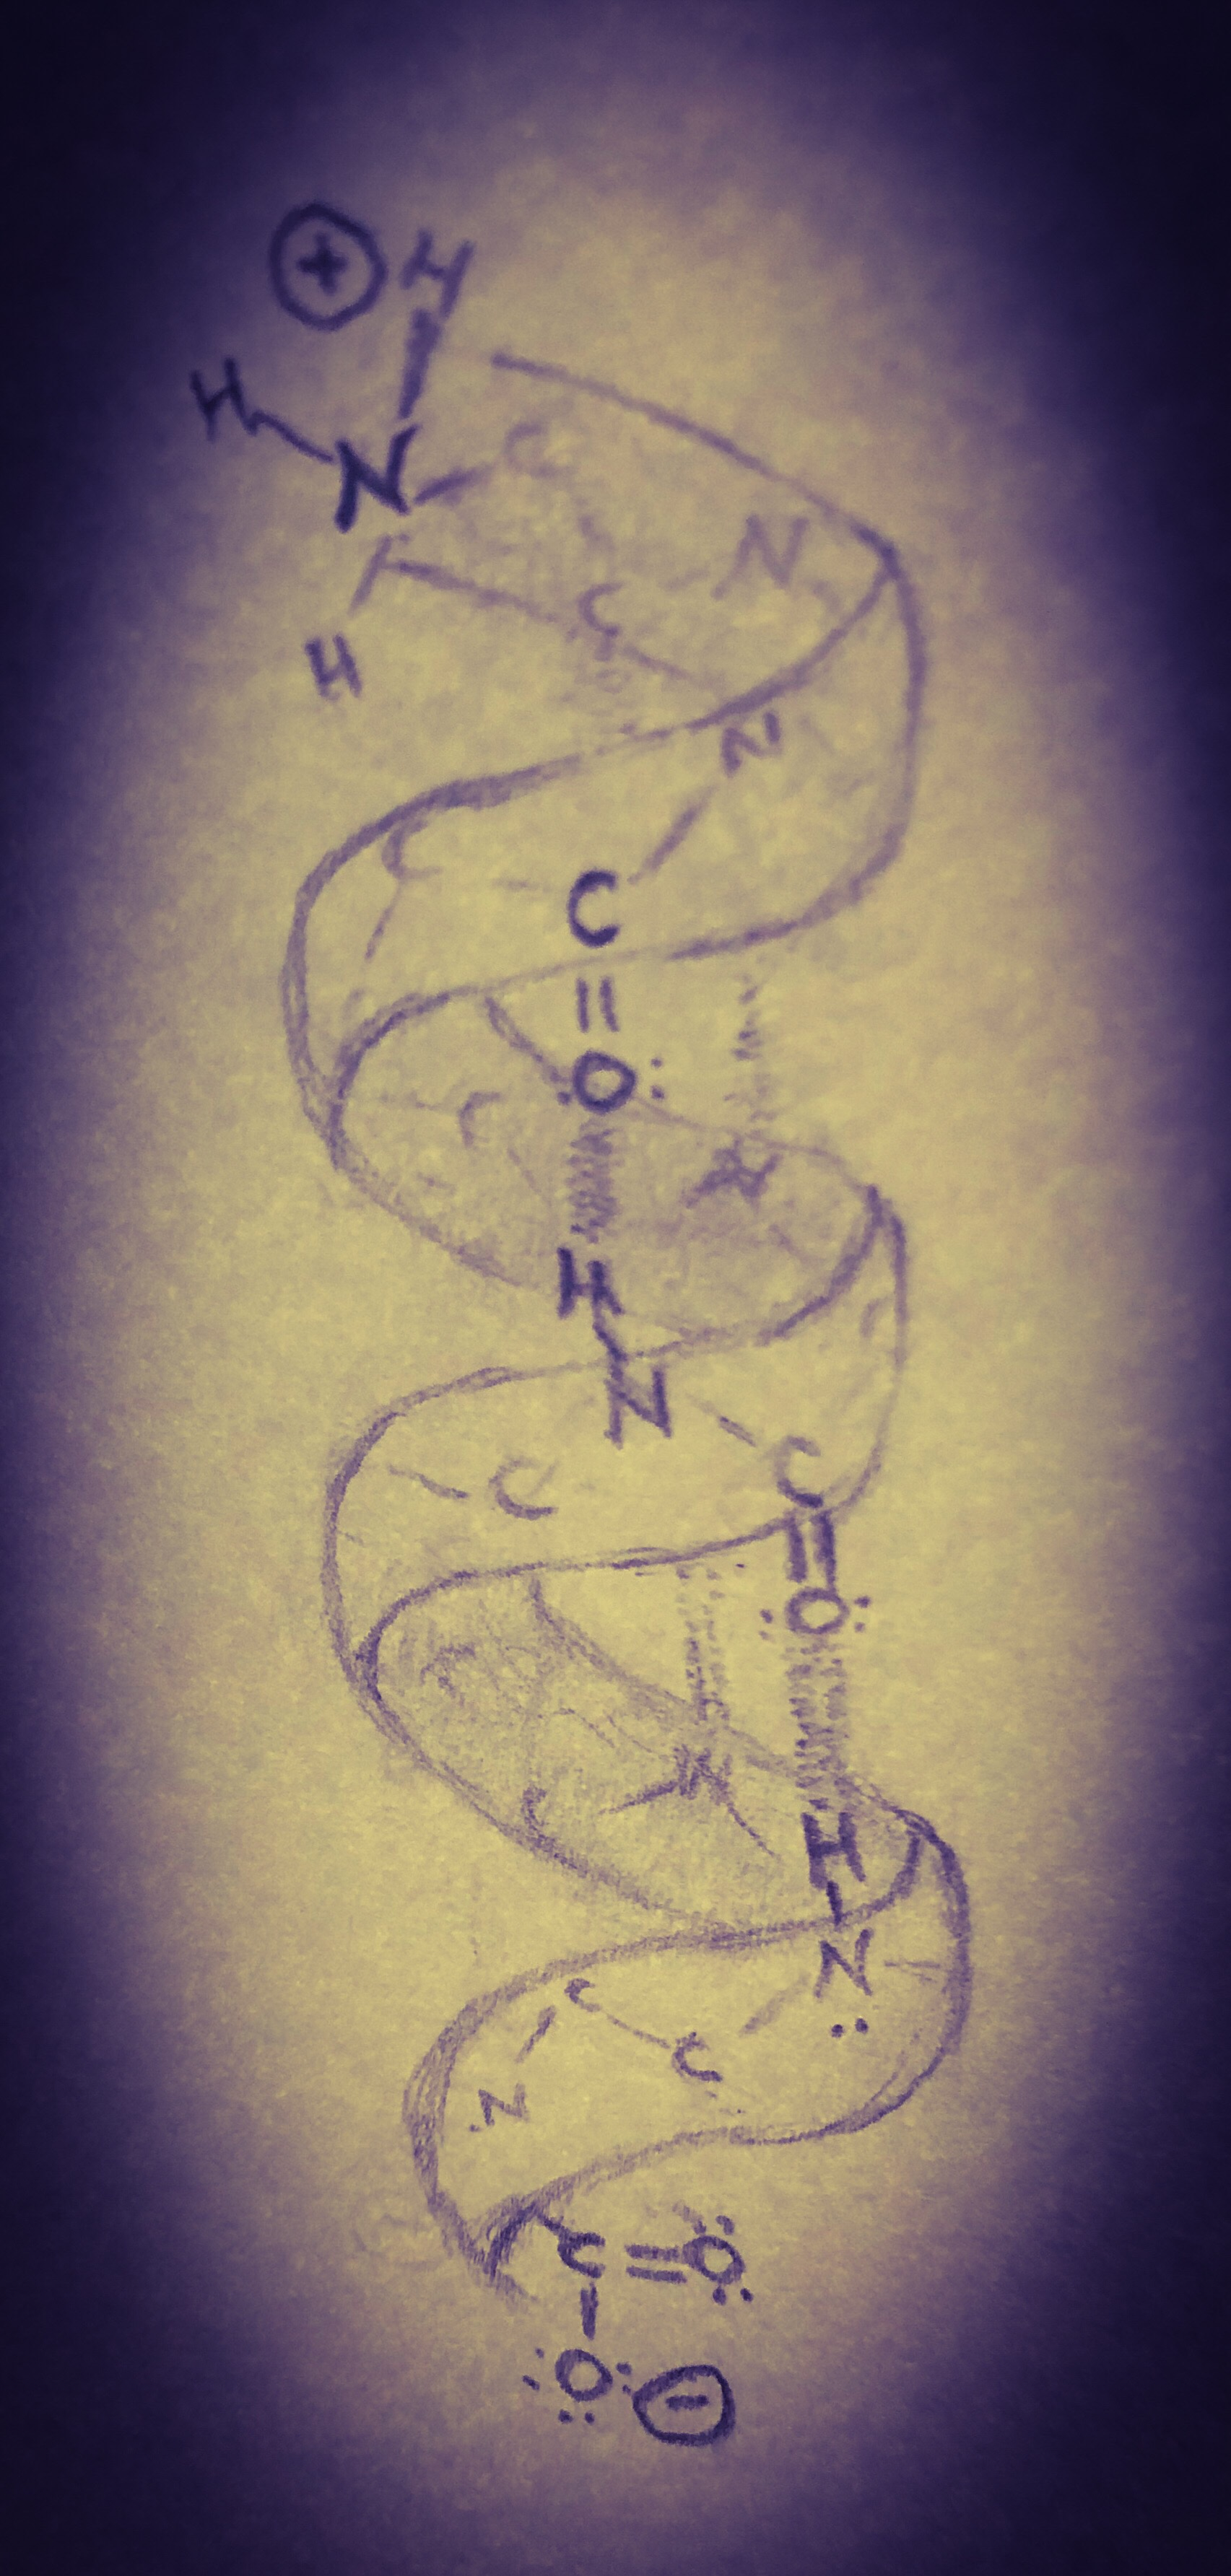
\includegraphics[width=0.6\linewidth]{helix.jpg}
        \caption{}\label{fig:fig_a}
\end{subfigure}
%
\begin{subfigure}[t]{.4\textwidth}
\centering
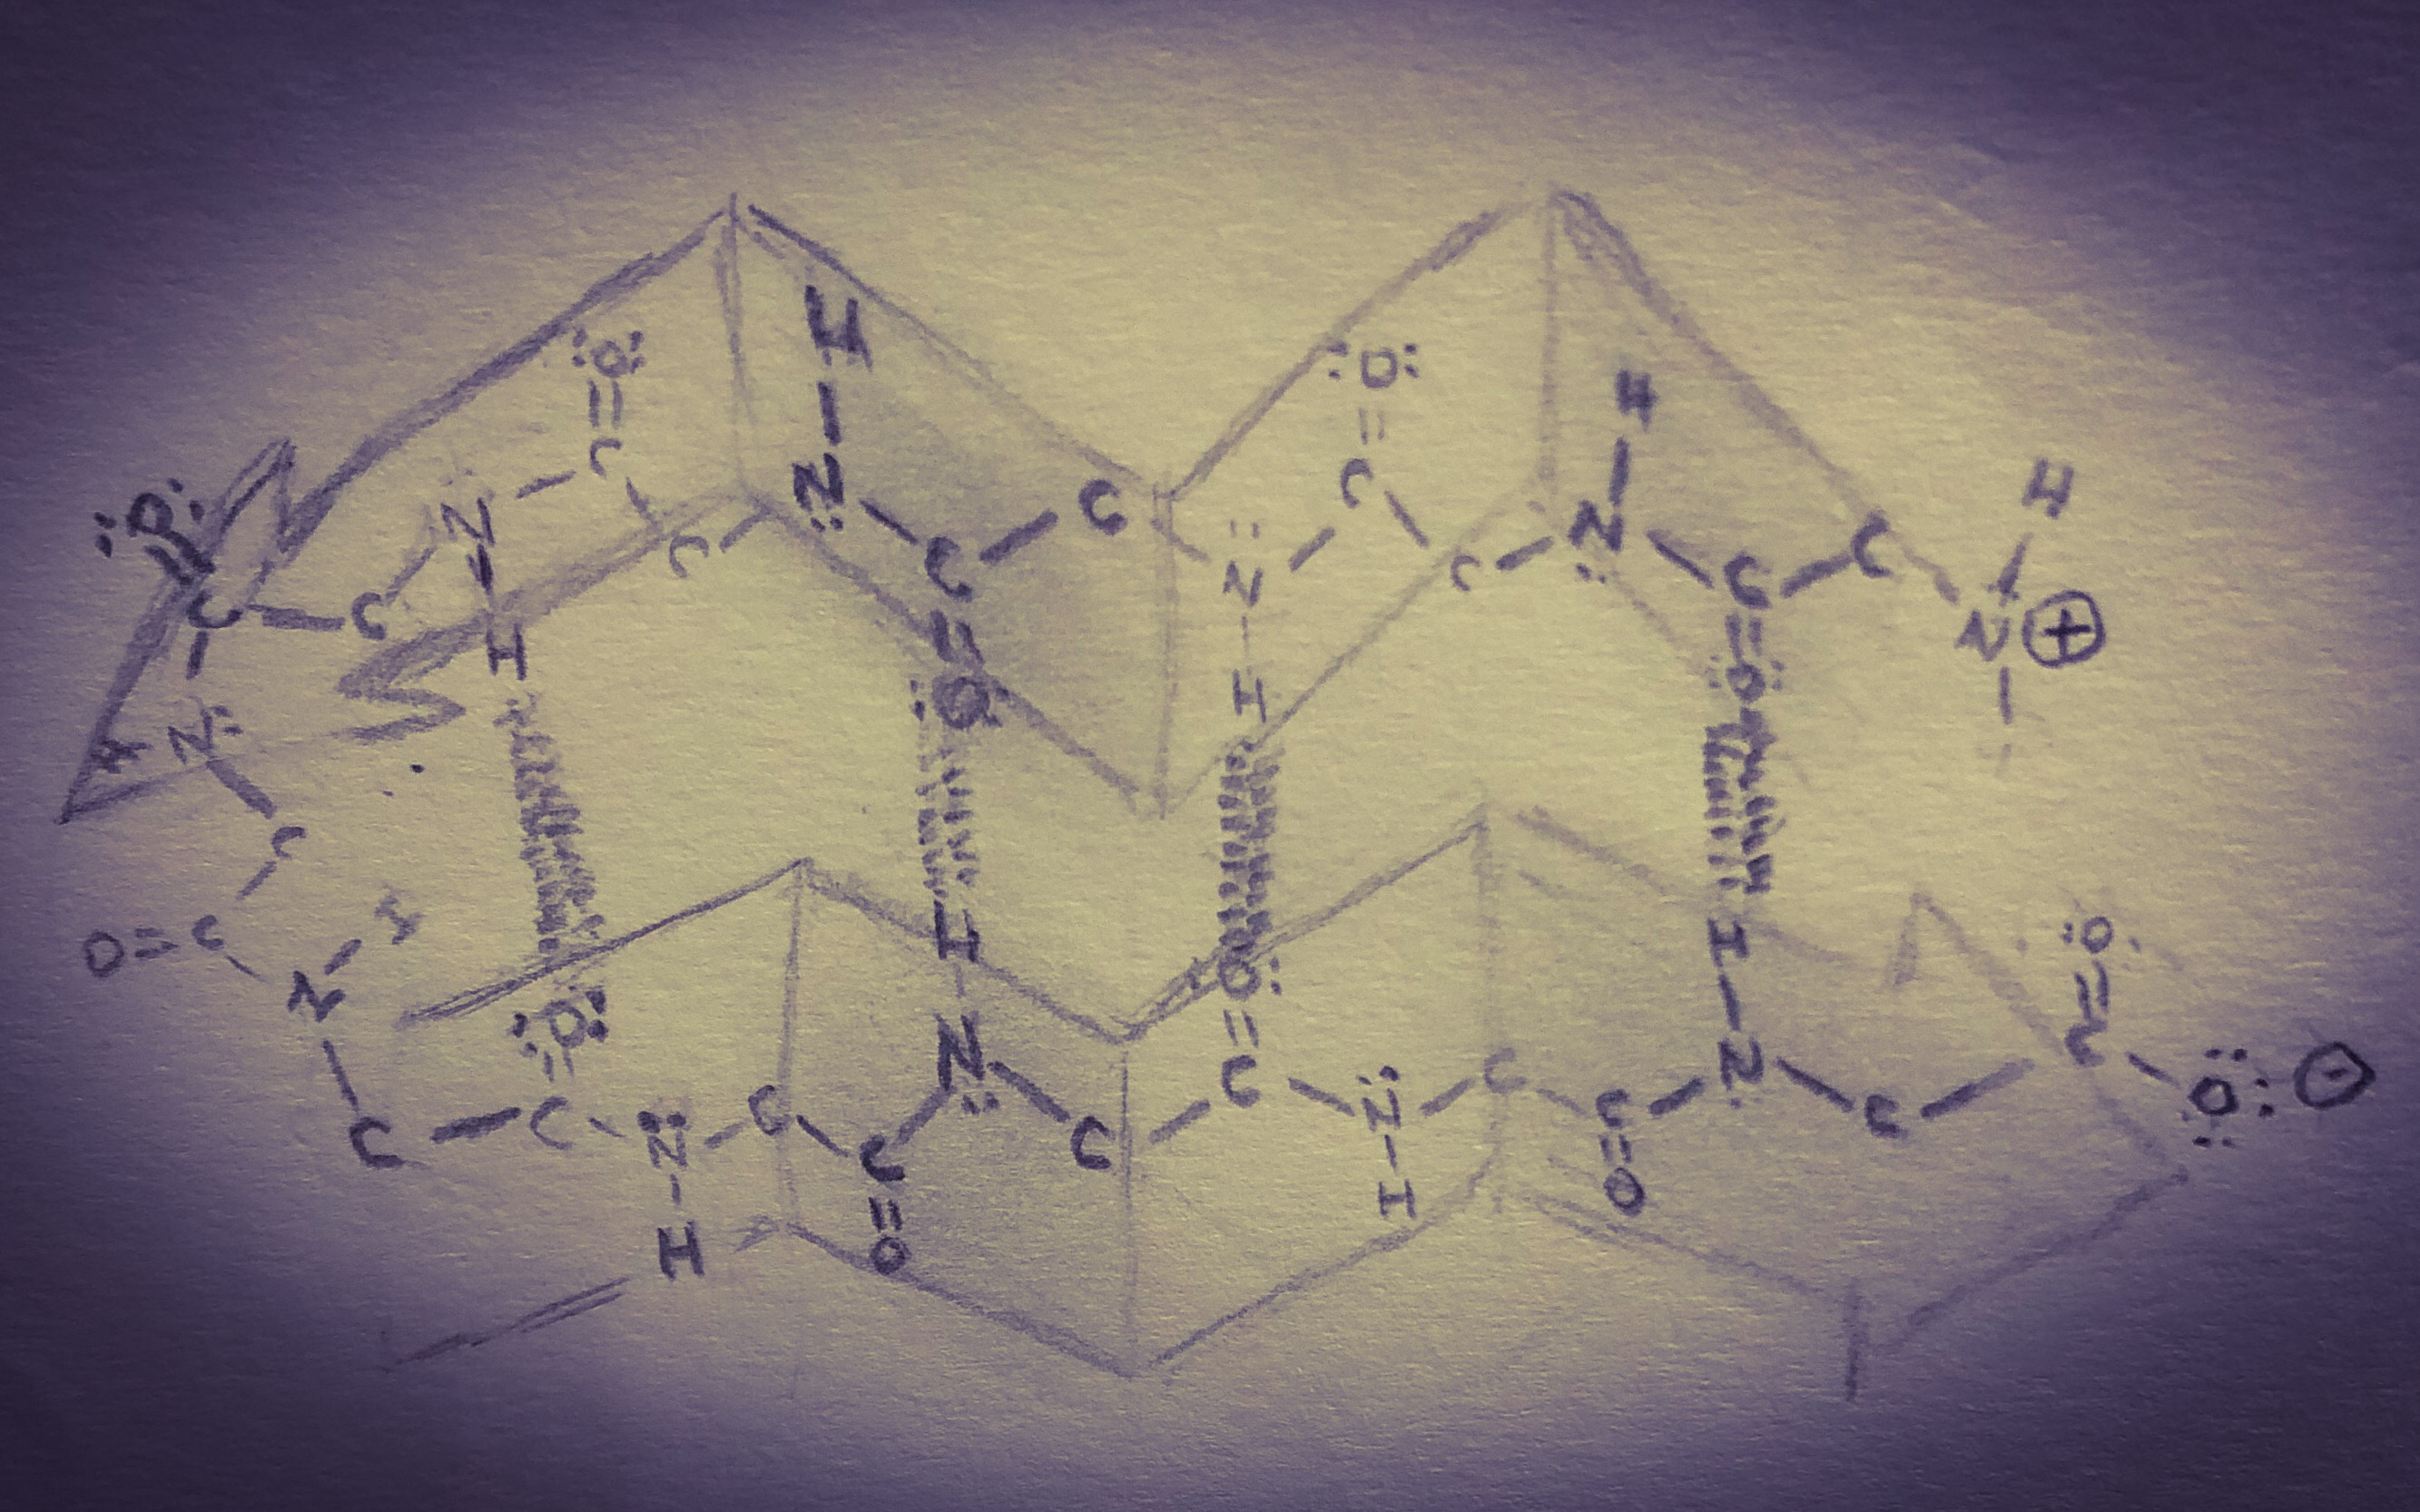
\includegraphics[width=1.3\linewidth]{sheet.jpg}
\caption{}\label{fig:fig_b}
\end{subfigure}



\begin{subfigure}[t]{.4\textwidth}
\centering
\vspace{0pt}% set the real top as the top
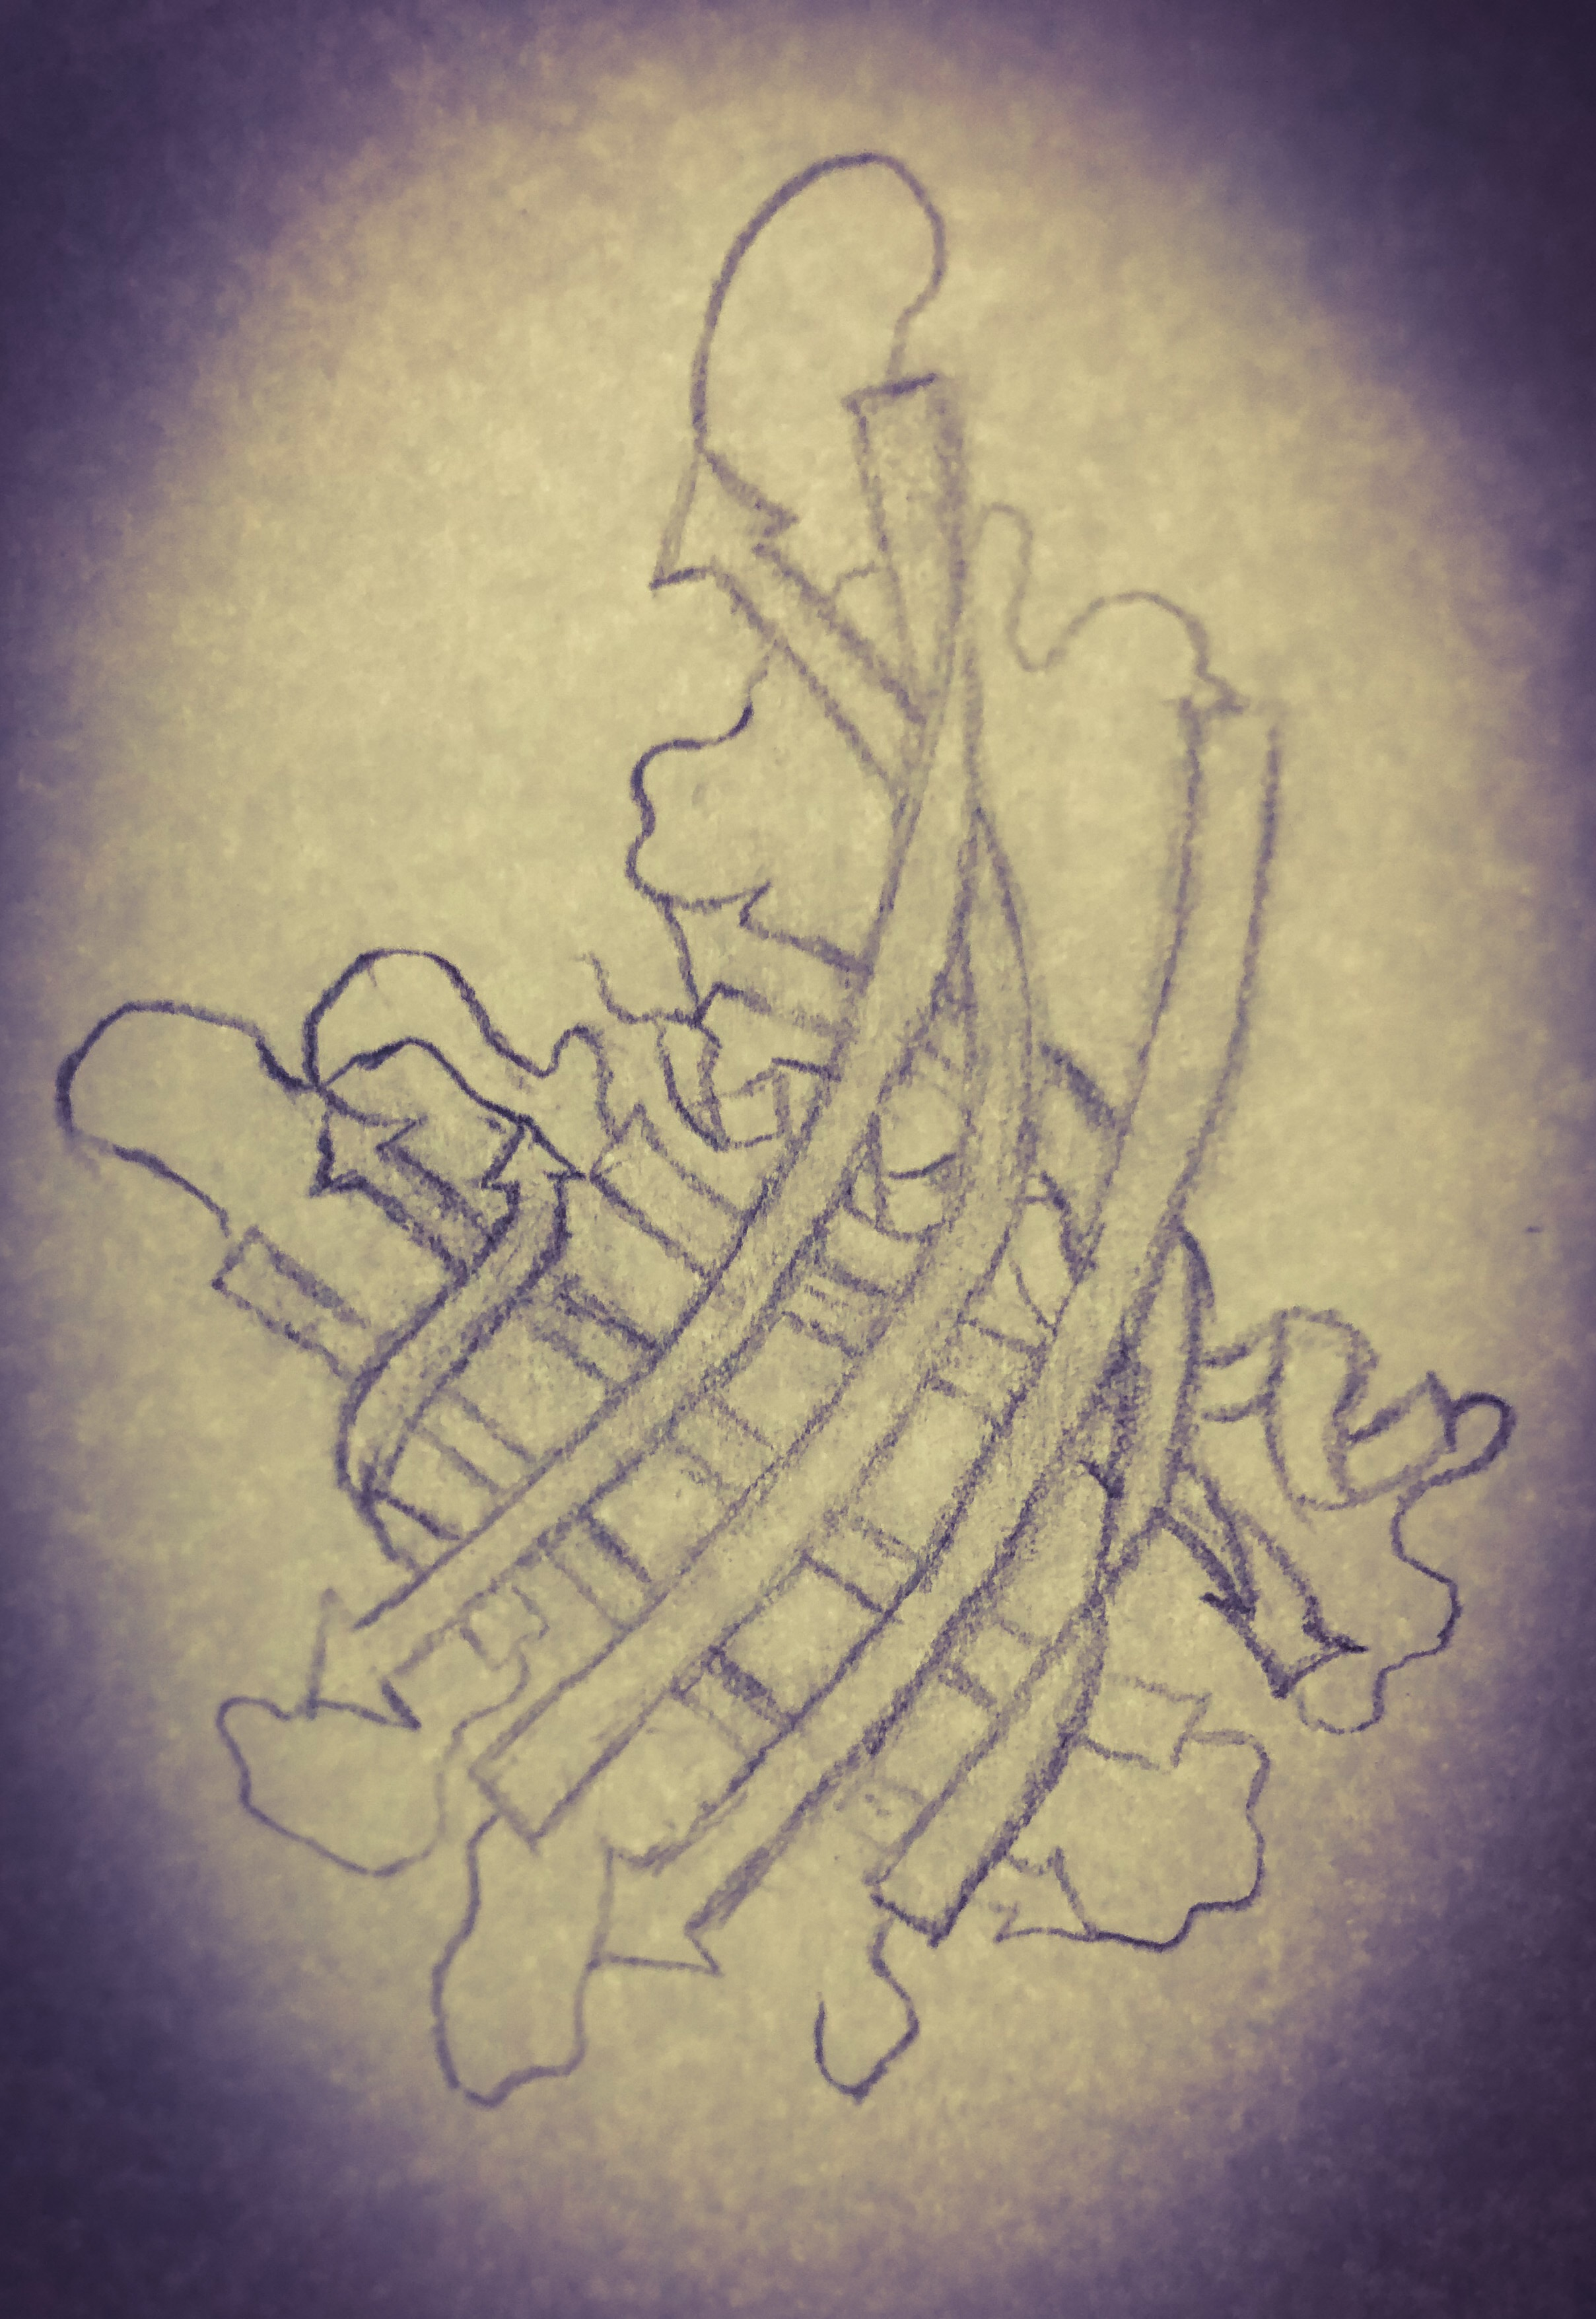
\includegraphics[width=\linewidth]{tertiary.jpg}
\caption{}\label{fig:fig_c}
\end{subfigure}
%
\begin{minipage}[t]{.5\textwidth}
\caption{Levels of protein structure (\subref{fig:fig_a}) $\alpha$-helix structure. (\subref{fig:fig_b}) parallel $\beta$-sheet structure.(\subref{fig:fig_c})tertiary structure comprised of a $\beta$-barrel and $\alpha$-helical moiety. }
\end{minipage}

\end{figure}
\end{comment}

\appendix


% Stuff at the end of the dissertation goes in the back matter
\backmatter
\bibliographystyle{plain} % Or whatever style you want like plainnat
\bibliography{library}

\end{document}
